% \pragmaonce

% adapted from https://www.overleaf.com/learn/latex/Commands
\providecommand{\dissertationexclude}[1]{%
% adapted from https://tex.stackexchange.com/a/33577
\ifdefined\DISSERTATION
\else
#1
\fi
}


\dissertationexclude{\clearpage}
\dissertationexclude{\onecolumn}

% \pragmaonce

% adapted from https://www.overleaf.com/learn/latex/Commands
\providecommand{\dissertationelse}[2]{%
% adapted from https://tex.stackexchange.com/a/33577
\ifdefined\DISSERTATION
#1
\else
#2
\fi
}


\newcommand{\tinyurl}[1]{\dissertationelse{\fontsize{8}{8}\selectfont}{\tiny}\url{#1}}

\newcommand{\morphcode}[1]{ \raisebox{-0.8em}{\color[HTML]{FFFFFF} \large \textbf{#1} }}

% \begin{table*}
\begin{longtable}[]{ccp{2.5cm} p{2.5cm} p{2.5cm} p{2.5cm} p{2.5cm}}
% \begin{tabular}{ccl}
\caption{Qualitative morph categorization of representative specimens sampled across evolutionary stints.
Video links provide an time-lapse animation of each specimen's morphology when grown in monoculture.
Web viewer URLs link to an in-browser simulation of each genome or population.
Human Readable genome link will download the corresponding genome as an annotated JSON file.} \label{tab:morph_by_stint} \\
\multicolumn{1}{l}{\textbf{Stint}}               & \textbf{Morph} & \textbf{Monoculture Video Link} & \textbf{Monoculture Web Viewer Link} & \textbf{Population Web Viewer Link} & \textbf{Human Readable Genome Link} \\
\endfirsthead
\caption*{\tablename{} \thetable{} (cont'd)} \\
\multicolumn{1}{l}{\textbf{Stint}}               & \textbf{Morph} & \textbf{Monoculture Video Link} & \textbf{Monoculture Web Viewer Link} & \textbf{Population Web Viewer Link} & \textbf{Human Readable Genome Link} \\
\endhead
0 & \cellcolor[HTML]{4C72B0}{\morphcode{a}} & \tinyurl{https://hopth.ru/21/b=prq49+s=16005+t=0+v=video+w=specimen} & \tinyurl{https://hopth.ru/21/b=prq49+s=16005+t=0+v=simulation+w=specimen} & \tinyurl{https://hopth.ru/21/b=prq49+s=16005+t=0+v=simulation+w=population} & \tinyurl{https://hopth.ru/21/b=prq49+s=16005+t=0+v=text+w=specimen} & \\
1 & \cellcolor[HTML]{DD8452}{\morphcode{b} } & \tinyurl{https://hopth.ru/21/b=prq49+s=16005+t=1+v=video+w=specimen} & \tinyurl{https://hopth.ru/21/b=prq49+s=16005+t=1+v=simulation+w=specimen} & \tinyurl{https://hopth.ru/21/b=prq49+s=16005+t=1+v=simulation+w=population} & \tinyurl{https://hopth.ru/21/b=prq49+s=16005+t=1+v=text+w=specimen} \\
2 & \cellcolor[HTML]{55A868}{\morphcode{c} } & \tinyurl{https://hopth.ru/21/b=prq49+s=16005+t=2+v=video+w=specimen} & \tinyurl{https://hopth.ru/21/b=prq49+s=16005+t=2+v=simulation+w=specimen} & \tinyurl{https://hopth.ru/21/b=prq49+s=16005+t=2+v=simulation+w=population} & \tinyurl{https://hopth.ru/21/b=prq49+s=16005+t=2+v=text+w=specimen} \\
3 & \cellcolor[HTML]{DD8452}{\morphcode{b} } & \tinyurl{https://hopth.ru/21/b=prq49+s=16005+t=3+v=video+w=specimen} & \tinyurl{https://hopth.ru/21/b=prq49+s=16005+t=3+v=simulation+w=specimen} & \tinyurl{https://hopth.ru/21/b=prq49+s=16005+t=3+v=simulation+w=population} & \tinyurl{https://hopth.ru/21/b=prq49+s=16005+t=3+v=text+w=specimen} \\
4 & \cellcolor[HTML]{DD8452}{\morphcode{b} } & \tinyurl{https://hopth.ru/21/b=prq49+s=16005+t=4+v=video+w=specimen} & \tinyurl{https://hopth.ru/21/b=prq49+s=16005+t=4+v=simulation+w=specimen} & \tinyurl{https://hopth.ru/21/b=prq49+s=16005+t=4+v=simulation+w=population} & \tinyurl{https://hopth.ru/21/b=prq49+s=16005+t=4+v=text+w=specimen} \\
5 & \cellcolor[HTML]{DD8452}{\morphcode{b} } & \tinyurl{https://hopth.ru/21/b=prq49+s=16005+t=5+v=video+w=specimen} & \tinyurl{https://hopth.ru/21/b=prq49+s=16005+t=5+v=simulation+w=specimen} & \tinyurl{https://hopth.ru/21/b=prq49+s=16005+t=5+v=simulation+w=population} & \tinyurl{https://hopth.ru/21/b=prq49+s=16005+t=5+v=text+w=specimen} \\
6 & \cellcolor[HTML]{DD8452}{\morphcode{b} } & \tinyurl{https://hopth.ru/21/b=prq49+s=16005+t=6+v=video+w=specimen} & \tinyurl{https://hopth.ru/21/b=prq49+s=16005+t=6+v=simulation+w=specimen} & \tinyurl{https://hopth.ru/21/b=prq49+s=16005+t=6+v=simulation+w=population} & \tinyurl{https://hopth.ru/21/b=prq49+s=16005+t=6+v=text+w=specimen} \\
7 & \cellcolor[HTML]{DD8452}{\morphcode{b} } & \tinyurl{https://hopth.ru/21/b=prq49+s=16005+t=7+v=video+w=specimen} & \tinyurl{https://hopth.ru/21/b=prq49+s=16005+t=7+v=simulation+w=specimen} & \tinyurl{https://hopth.ru/21/b=prq49+s=16005+t=7+v=simulation+w=population} & \tinyurl{https://hopth.ru/21/b=prq49+s=16005+t=7+v=text+w=specimen} \\
8 & \cellcolor[HTML]{DD8452}{\morphcode{b} } & \tinyurl{https://hopth.ru/21/b=prq49+s=16005+t=8+v=video+w=specimen} & \tinyurl{https://hopth.ru/21/b=prq49+s=16005+t=8+v=simulation+w=specimen} & \tinyurl{https://hopth.ru/21/b=prq49+s=16005+t=8+v=simulation+w=population} & \tinyurl{https://hopth.ru/21/b=prq49+s=16005+t=8+v=text+w=specimen} \\
9 & \cellcolor[HTML]{DD8452}{\morphcode{b} } & \tinyurl{https://hopth.ru/21/b=prq49+s=16005+t=9+v=video+w=specimen} & \tinyurl{https://hopth.ru/21/b=prq49+s=16005+t=9+v=simulation+w=specimen} & \tinyurl{https://hopth.ru/21/b=prq49+s=16005+t=9+v=simulation+w=population} & \tinyurl{https://hopth.ru/21/b=prq49+s=16005+t=9+v=text+w=specimen} \\
10 & \cellcolor[HTML]{DD8452}{\morphcode{b} } & \tinyurl{https://hopth.ru/21/b=prq49+s=16005+t=10+v=video+w=specimen} & \tinyurl{https://hopth.ru/21/b=prq49+s=16005+t=10+v=simulation+w=specimen} & \tinyurl{https://hopth.ru/21/b=prq49+s=16005+t=10+v=simulation+w=population} & \tinyurl{https://hopth.ru/21/b=prq49+s=16005+t=10+v=text+w=specimen} \\
11 & \cellcolor[HTML]{DD8452}{\morphcode{b} } & \tinyurl{https://hopth.ru/21/b=prq49+s=16005+t=11+v=video+w=specimen} & \tinyurl{https://hopth.ru/21/b=prq49+s=16005+t=11+v=simulation+w=specimen} & \tinyurl{https://hopth.ru/21/b=prq49+s=16005+t=11+v=simulation+w=population} & \tinyurl{https://hopth.ru/21/b=prq49+s=16005+t=11+v=text+w=specimen} \\
12 & \cellcolor[HTML]{DD8452}{\morphcode{b} } & \tinyurl{https://hopth.ru/21/b=prq49+s=16005+t=12+v=video+w=specimen} & \tinyurl{https://hopth.ru/21/b=prq49+s=16005+t=12+v=simulation+w=specimen} & \tinyurl{https://hopth.ru/21/b=prq49+s=16005+t=12+v=simulation+w=population} & \tinyurl{https://hopth.ru/21/b=prq49+s=16005+t=12+v=text+w=specimen} \\
13 & \cellcolor[HTML]{DD8452}{\morphcode{b} } & \tinyurl{https://hopth.ru/21/b=prq49+s=16005+t=13+v=video+w=specimen} & \tinyurl{https://hopth.ru/21/b=prq49+s=16005+t=13+v=simulation+w=specimen} & \tinyurl{https://hopth.ru/21/b=prq49+s=16005+t=13+v=simulation+w=population} & \tinyurl{https://hopth.ru/21/b=prq49+s=16005+t=13+v=text+w=specimen} \\
14 & \cellcolor[HTML]{C44E52}{\morphcode{d} } & \tinyurl{https://hopth.ru/21/b=prq49+s=16005+t=14+v=video+w=specimen} & \tinyurl{https://hopth.ru/21/b=prq49+s=16005+t=14+v=simulation+w=specimen} & \tinyurl{https://hopth.ru/21/b=prq49+s=16005+t=14+v=simulation+w=population} & \tinyurl{https://hopth.ru/21/b=prq49+s=16005+t=14+v=text+w=specimen} \\
15 & \cellcolor[HTML]{8172B3}{\morphcode{e} } & \tinyurl{https://hopth.ru/21/b=prq49+s=16005+t=15+v=video+w=specimen} & \tinyurl{https://hopth.ru/21/b=prq49+s=16005+t=15+v=simulation+w=specimen} & \tinyurl{https://hopth.ru/21/b=prq49+s=16005+t=15+v=simulation+w=population} & \tinyurl{https://hopth.ru/21/b=prq49+s=16005+t=15+v=text+w=specimen} \\
16 & \cellcolor[HTML]{8172B3}{\morphcode{e} } & \tinyurl{https://hopth.ru/21/b=prq49+s=16005+t=16+v=video+w=specimen} & \tinyurl{https://hopth.ru/21/b=prq49+s=16005+t=16+v=simulation+w=specimen} & \tinyurl{https://hopth.ru/21/b=prq49+s=16005+t=16+v=simulation+w=population} & \tinyurl{https://hopth.ru/21/b=prq49+s=16005+t=16+v=text+w=specimen} \\
17 & \cellcolor[HTML]{8172B3}{\morphcode{e} } & \tinyurl{https://hopth.ru/21/b=prq49+s=16005+t=17+v=video+w=specimen} & \tinyurl{https://hopth.ru/21/b=prq49+s=16005+t=17+v=simulation+w=specimen} & \tinyurl{https://hopth.ru/21/b=prq49+s=16005+t=17+v=simulation+w=population} & \tinyurl{https://hopth.ru/21/b=prq49+s=16005+t=17+v=text+w=specimen} \\
18 & \cellcolor[HTML]{8172B3}{\morphcode{e} } & \tinyurl{https://hopth.ru/21/b=prq49+s=16005+t=18+v=video+w=specimen} & \tinyurl{https://hopth.ru/21/b=prq49+s=16005+t=18+v=simulation+w=specimen} & \tinyurl{https://hopth.ru/21/b=prq49+s=16005+t=18+v=simulation+w=population} & \tinyurl{https://hopth.ru/21/b=prq49+s=16005+t=18+v=text+w=specimen} \\
19 & \cellcolor[HTML]{8172B3}{\morphcode{e} } & \tinyurl{https://hopth.ru/21/b=prq49+s=16005+t=19+v=video+w=specimen} & \tinyurl{https://hopth.ru/21/b=prq49+s=16005+t=19+v=simulation+w=specimen} & \tinyurl{https://hopth.ru/21/b=prq49+s=16005+t=19+v=simulation+w=population} & \tinyurl{https://hopth.ru/21/b=prq49+s=16005+t=19+v=text+w=specimen} \\
20 & \cellcolor[HTML]{8172B3}{\morphcode{e} } & \tinyurl{https://hopth.ru/21/b=prq49+s=16005+t=20+v=video+w=specimen} & \tinyurl{https://hopth.ru/21/b=prq49+s=16005+t=20+v=simulation+w=specimen} & \tinyurl{https://hopth.ru/21/b=prq49+s=16005+t=20+v=simulation+w=population} & \tinyurl{https://hopth.ru/21/b=prq49+s=16005+t=20+v=text+w=specimen} \\
21 & \cellcolor[HTML]{8172B3}{\morphcode{e} } & \tinyurl{https://hopth.ru/21/b=prq49+s=16005+t=21+v=video+w=specimen} & \tinyurl{https://hopth.ru/21/b=prq49+s=16005+t=21+v=simulation+w=specimen} & \tinyurl{https://hopth.ru/21/b=prq49+s=16005+t=21+v=simulation+w=population} & \tinyurl{https://hopth.ru/21/b=prq49+s=16005+t=21+v=text+w=specimen} \\
22 & \cellcolor[HTML]{8172B3}{\morphcode{e} } & \tinyurl{https://hopth.ru/21/b=prq49+s=16005+t=22+v=video+w=specimen} & \tinyurl{https://hopth.ru/21/b=prq49+s=16005+t=22+v=simulation+w=specimen} & \tinyurl{https://hopth.ru/21/b=prq49+s=16005+t=22+v=simulation+w=population} & \tinyurl{https://hopth.ru/21/b=prq49+s=16005+t=22+v=text+w=specimen} \\
23 & \cellcolor[HTML]{8172B3}{\morphcode{e} } & \tinyurl{https://hopth.ru/21/b=prq49+s=16005+t=23+v=video+w=specimen} & \tinyurl{https://hopth.ru/21/b=prq49+s=16005+t=23+v=simulation+w=specimen} & \tinyurl{https://hopth.ru/21/b=prq49+s=16005+t=23+v=simulation+w=population} & \tinyurl{https://hopth.ru/21/b=prq49+s=16005+t=23+v=text+w=specimen} \\
24 & \cellcolor[HTML]{8172B3}{\morphcode{e} } & \tinyurl{https://hopth.ru/21/b=prq49+s=16005+t=24+v=video+w=specimen} & \tinyurl{https://hopth.ru/21/b=prq49+s=16005+t=24+v=simulation+w=specimen} & \tinyurl{https://hopth.ru/21/b=prq49+s=16005+t=24+v=simulation+w=population} & \tinyurl{https://hopth.ru/21/b=prq49+s=16005+t=24+v=text+w=specimen} \\
25 & \cellcolor[HTML]{8172B3}{\morphcode{e} } & \tinyurl{https://hopth.ru/21/b=prq49+s=16005+t=25+v=video+w=specimen} & \tinyurl{https://hopth.ru/21/b=prq49+s=16005+t=25+v=simulation+w=specimen} & \tinyurl{https://hopth.ru/21/b=prq49+s=16005+t=25+v=simulation+w=population} & \tinyurl{https://hopth.ru/21/b=prq49+s=16005+t=25+v=text+w=specimen} \\
26 & \cellcolor[HTML]{DD8452}{\morphcode{b} } & \tinyurl{https://hopth.ru/21/b=prq49+s=16005+t=26+v=video+w=specimen} & \tinyurl{https://hopth.ru/21/b=prq49+s=16005+t=26+v=simulation+w=specimen} & \tinyurl{https://hopth.ru/21/b=prq49+s=16005+t=26+v=simulation+w=population} & \tinyurl{https://hopth.ru/21/b=prq49+s=16005+t=26+v=text+w=specimen} \\
27 & \cellcolor[HTML]{8172B3}{\morphcode{e} } & \tinyurl{https://hopth.ru/21/b=prq49+s=16005+t=27+v=video+w=specimen} & \tinyurl{https://hopth.ru/21/b=prq49+s=16005+t=27+v=simulation+w=specimen} & \tinyurl{https://hopth.ru/21/b=prq49+s=16005+t=27+v=simulation+w=population} & \tinyurl{https://hopth.ru/21/b=prq49+s=16005+t=27+v=text+w=specimen} \\
28 & \cellcolor[HTML]{DD8452}{\morphcode{b} } & \tinyurl{https://hopth.ru/21/b=prq49+s=16005+t=28+v=video+w=specimen} & \tinyurl{https://hopth.ru/21/b=prq49+s=16005+t=28+v=simulation+w=specimen} & \tinyurl{https://hopth.ru/21/b=prq49+s=16005+t=28+v=simulation+w=population} & \tinyurl{https://hopth.ru/21/b=prq49+s=16005+t=28+v=text+w=specimen} \\
29 & \cellcolor[HTML]{8172B3}{\morphcode{e} } & \tinyurl{https://hopth.ru/21/b=prq49+s=16005+t=29+v=video+w=specimen} & \tinyurl{https://hopth.ru/21/b=prq49+s=16005+t=29+v=simulation+w=specimen} & \tinyurl{https://hopth.ru/21/b=prq49+s=16005+t=29+v=simulation+w=population} & \tinyurl{https://hopth.ru/21/b=prq49+s=16005+t=29+v=text+w=specimen} \\
30 & \cellcolor[HTML]{8172B3}{\morphcode{e} } & \tinyurl{https://hopth.ru/21/b=prq49+s=16005+t=30+v=video+w=specimen} & \tinyurl{https://hopth.ru/21/b=prq49+s=16005+t=30+v=simulation+w=specimen} & \tinyurl{https://hopth.ru/21/b=prq49+s=16005+t=30+v=simulation+w=population} & \tinyurl{https://hopth.ru/21/b=prq49+s=16005+t=30+v=text+w=specimen} \\
31 & \cellcolor[HTML]{8172B3}{\morphcode{e} } & \tinyurl{https://hopth.ru/21/b=prq49+s=16005+t=31+v=video+w=specimen} & \tinyurl{https://hopth.ru/21/b=prq49+s=16005+t=31+v=simulation+w=specimen} & \tinyurl{https://hopth.ru/21/b=prq49+s=16005+t=31+v=simulation+w=population} & \tinyurl{https://hopth.ru/21/b=prq49+s=16005+t=31+v=text+w=specimen} \\
32 & \cellcolor[HTML]{8172B3}{\morphcode{e} } & \tinyurl{https://hopth.ru/21/b=prq49+s=16005+t=32+v=video+w=specimen} & \tinyurl{https://hopth.ru/21/b=prq49+s=16005+t=32+v=simulation+w=specimen} & \tinyurl{https://hopth.ru/21/b=prq49+s=16005+t=32+v=simulation+w=population} & \tinyurl{https://hopth.ru/21/b=prq49+s=16005+t=32+v=text+w=specimen} \\
33 & \cellcolor[HTML]{8172B3}{\morphcode{e} } & \tinyurl{https://hopth.ru/21/b=prq49+s=16005+t=33+v=video+w=specimen} & \tinyurl{https://hopth.ru/21/b=prq49+s=16005+t=33+v=simulation+w=specimen} & \tinyurl{https://hopth.ru/21/b=prq49+s=16005+t=33+v=simulation+w=population} & \tinyurl{https://hopth.ru/21/b=prq49+s=16005+t=33+v=text+w=specimen} \\
34 & \cellcolor[HTML]{8172B3}{\morphcode{e} } & \tinyurl{https://hopth.ru/21/b=prq49+s=16005+t=34+v=video+w=specimen} & \tinyurl{https://hopth.ru/21/b=prq49+s=16005+t=34+v=simulation+w=specimen} & \tinyurl{https://hopth.ru/21/b=prq49+s=16005+t=34+v=simulation+w=population} & \tinyurl{https://hopth.ru/21/b=prq49+s=16005+t=34+v=text+w=specimen} \\
35 & \cellcolor[HTML]{8172B3}{\morphcode{e} } & \tinyurl{https://hopth.ru/21/b=prq49+s=16005+t=35+v=video+w=specimen} & \tinyurl{https://hopth.ru/21/b=prq49+s=16005+t=35+v=simulation+w=specimen} & \tinyurl{https://hopth.ru/21/b=prq49+s=16005+t=35+v=simulation+w=population} & \tinyurl{https://hopth.ru/21/b=prq49+s=16005+t=35+v=text+w=specimen} \\
36 & \cellcolor[HTML]{8172B3}{\morphcode{e} } & \tinyurl{https://hopth.ru/21/b=prq49+s=16005+t=36+v=video+w=specimen} & \tinyurl{https://hopth.ru/21/b=prq49+s=16005+t=36+v=simulation+w=specimen} & \tinyurl{https://hopth.ru/21/b=prq49+s=16005+t=36+v=simulation+w=population} & \tinyurl{https://hopth.ru/21/b=prq49+s=16005+t=36+v=text+w=specimen} \\
37 & \cellcolor[HTML]{8172B3}{\morphcode{e} } & \tinyurl{https://hopth.ru/21/b=prq49+s=16005+t=37+v=video+w=specimen} & \tinyurl{https://hopth.ru/21/b=prq49+s=16005+t=37+v=simulation+w=specimen} & \tinyurl{https://hopth.ru/21/b=prq49+s=16005+t=37+v=simulation+w=population} & \tinyurl{https://hopth.ru/21/b=prq49+s=16005+t=37+v=text+w=specimen} \\
38 & \cellcolor[HTML]{8172B3}{\morphcode{e} } & \tinyurl{https://hopth.ru/21/b=prq49+s=16005+t=38+v=video+w=specimen} & \tinyurl{https://hopth.ru/21/b=prq49+s=16005+t=38+v=simulation+w=specimen} & \tinyurl{https://hopth.ru/21/b=prq49+s=16005+t=38+v=simulation+w=population} & \tinyurl{https://hopth.ru/21/b=prq49+s=16005+t=38+v=text+w=specimen} \\
39 & \cellcolor[HTML]{937860}{\morphcode{f} } & \tinyurl{https://hopth.ru/21/b=prq49+s=16005+t=39+v=video+w=specimen} & \tinyurl{https://hopth.ru/21/b=prq49+s=16005+t=39+v=simulation+w=specimen} & \tinyurl{https://hopth.ru/21/b=prq49+s=16005+t=39+v=simulation+w=population} & \tinyurl{https://hopth.ru/21/b=prq49+s=16005+t=39+v=text+w=specimen} \\
40 & \cellcolor[HTML]{8172B3}{\morphcode{e} } & \tinyurl{https://hopth.ru/21/b=prq49+s=16005+t=40+v=video+w=specimen} & \tinyurl{https://hopth.ru/21/b=prq49+s=16005+t=40+v=simulation+w=specimen} & \tinyurl{https://hopth.ru/21/b=prq49+s=16005+t=40+v=simulation+w=population} & \tinyurl{https://hopth.ru/21/b=prq49+s=16005+t=40+v=text+w=specimen} \\
41 & \cellcolor[HTML]{8172B3}{\morphcode{e} } & \tinyurl{https://hopth.ru/21/b=prq49+s=16005+t=41+v=video+w=specimen} & \tinyurl{https://hopth.ru/21/b=prq49+s=16005+t=41+v=simulation+w=specimen} & \tinyurl{https://hopth.ru/21/b=prq49+s=16005+t=41+v=simulation+w=population} & \tinyurl{https://hopth.ru/21/b=prq49+s=16005+t=41+v=text+w=specimen} \\
42 & \cellcolor[HTML]{8172B3}{\morphcode{e} } & \tinyurl{https://hopth.ru/21/b=prq49+s=16005+t=42+v=video+w=specimen} & \tinyurl{https://hopth.ru/21/b=prq49+s=16005+t=42+v=simulation+w=specimen} & \tinyurl{https://hopth.ru/21/b=prq49+s=16005+t=42+v=simulation+w=population} & \tinyurl{https://hopth.ru/21/b=prq49+s=16005+t=42+v=text+w=specimen} \\
43 & \cellcolor[HTML]{8172B3}{\morphcode{e} } & \tinyurl{https://hopth.ru/21/b=prq49+s=16005+t=43+v=video+w=specimen} & \tinyurl{https://hopth.ru/21/b=prq49+s=16005+t=43+v=simulation+w=specimen} & \tinyurl{https://hopth.ru/21/b=prq49+s=16005+t=43+v=simulation+w=population} & \tinyurl{https://hopth.ru/21/b=prq49+s=16005+t=43+v=text+w=specimen} \\
44 & \cellcolor[HTML]{8172B3}{\morphcode{e} } & \tinyurl{https://hopth.ru/21/b=prq49+s=16005+t=44+v=video+w=specimen} & \tinyurl{https://hopth.ru/21/b=prq49+s=16005+t=44+v=simulation+w=specimen} & \tinyurl{https://hopth.ru/21/b=prq49+s=16005+t=44+v=simulation+w=population} & \tinyurl{https://hopth.ru/21/b=prq49+s=16005+t=44+v=text+w=specimen} \\
45 & \cellcolor[HTML]{DA8BC3}{\morphcode{g} } & \tinyurl{https://hopth.ru/21/b=prq49+s=16005+t=45+v=video+w=specimen} & \tinyurl{https://hopth.ru/21/b=prq49+s=16005+t=45+v=simulation+w=specimen} & \tinyurl{https://hopth.ru/21/b=prq49+s=16005+t=45+v=simulation+w=population} & \tinyurl{https://hopth.ru/21/b=prq49+s=16005+t=45+v=text+w=specimen} \\
46 & \cellcolor[HTML]{DA8BC3}{\morphcode{g} } & \tinyurl{https://hopth.ru/21/b=prq49+s=16005+t=46+v=video+w=specimen} & \tinyurl{https://hopth.ru/21/b=prq49+s=16005+t=46+v=simulation+w=specimen} & \tinyurl{https://hopth.ru/21/b=prq49+s=16005+t=46+v=simulation+w=population} & \tinyurl{https://hopth.ru/21/b=prq49+s=16005+t=46+v=text+w=specimen} \\
47 & \cellcolor[HTML]{DA8BC3}{\morphcode{g} } & \tinyurl{https://hopth.ru/21/b=prq49+s=16005+t=47+v=video+w=specimen} & \tinyurl{https://hopth.ru/21/b=prq49+s=16005+t=47+v=simulation+w=specimen} & \tinyurl{https://hopth.ru/21/b=prq49+s=16005+t=47+v=simulation+w=population} & \tinyurl{https://hopth.ru/21/b=prq49+s=16005+t=47+v=text+w=specimen} \\
48 & \cellcolor[HTML]{DA8BC3}{\morphcode{g} } & \tinyurl{https://hopth.ru/21/b=prq49+s=16005+t=48+v=video+w=specimen} & \tinyurl{https://hopth.ru/21/b=prq49+s=16005+t=48+v=simulation+w=specimen} & \tinyurl{https://hopth.ru/21/b=prq49+s=16005+t=48+v=simulation+w=population} & \tinyurl{https://hopth.ru/21/b=prq49+s=16005+t=48+v=text+w=specimen} \\
49 & \cellcolor[HTML]{DA8BC3}{\morphcode{g} } & \tinyurl{https://hopth.ru/21/b=prq49+s=16005+t=49+v=video+w=specimen} & \tinyurl{https://hopth.ru/21/b=prq49+s=16005+t=49+v=simulation+w=specimen} & \tinyurl{https://hopth.ru/21/b=prq49+s=16005+t=49+v=simulation+w=population} & \tinyurl{https://hopth.ru/21/b=prq49+s=16005+t=49+v=text+w=specimen} \\
50 & \cellcolor[HTML]{DA8BC3}{\morphcode{g} } & \tinyurl{https://hopth.ru/21/b=prq49+s=16005+t=50+v=video+w=specimen} & \tinyurl{https://hopth.ru/21/b=prq49+s=16005+t=50+v=simulation+w=specimen} & \tinyurl{https://hopth.ru/21/b=prq49+s=16005+t=50+v=simulation+w=population} & \tinyurl{https://hopth.ru/21/b=prq49+s=16005+t=50+v=text+w=specimen} \\
51 & \cellcolor[HTML]{DA8BC3}{\morphcode{g} } & \tinyurl{https://hopth.ru/21/b=prq49+s=16005+t=51+v=video+w=specimen} & \tinyurl{https://hopth.ru/21/b=prq49+s=16005+t=51+v=simulation+w=specimen} & \tinyurl{https://hopth.ru/21/b=prq49+s=16005+t=51+v=simulation+w=population} & \tinyurl{https://hopth.ru/21/b=prq49+s=16005+t=51+v=text+w=specimen} \\
52 & \cellcolor[HTML]{DA8BC3}{\morphcode{g} } & \tinyurl{https://hopth.ru/21/b=prq49+s=16005+t=52+v=video+w=specimen} & \tinyurl{https://hopth.ru/21/b=prq49+s=16005+t=52+v=simulation+w=specimen} & \tinyurl{https://hopth.ru/21/b=prq49+s=16005+t=52+v=simulation+w=population} & \tinyurl{https://hopth.ru/21/b=prq49+s=16005+t=52+v=text+w=specimen} \\
53 & \cellcolor[HTML]{8172B3}{\morphcode{e} } & \tinyurl{https://hopth.ru/21/b=prq49+s=16005+t=53+v=video+w=specimen} & \tinyurl{https://hopth.ru/21/b=prq49+s=16005+t=53+v=simulation+w=specimen} & \tinyurl{https://hopth.ru/21/b=prq49+s=16005+t=53+v=simulation+w=population} & \tinyurl{https://hopth.ru/21/b=prq49+s=16005+t=53+v=text+w=specimen} \\
54 & \cellcolor[HTML]{DA8BC3}{\morphcode{g} } & \tinyurl{https://hopth.ru/21/b=prq49+s=16005+t=54+v=video+w=specimen} & \tinyurl{https://hopth.ru/21/b=prq49+s=16005+t=54+v=simulation+w=specimen} & \tinyurl{https://hopth.ru/21/b=prq49+s=16005+t=54+v=simulation+w=population} & \tinyurl{https://hopth.ru/21/b=prq49+s=16005+t=54+v=text+w=specimen} \\
55 & \cellcolor[HTML]{DA8BC3}{\morphcode{g} } & \tinyurl{https://hopth.ru/21/b=prq49+s=16005+t=55+v=video+w=specimen} & \tinyurl{https://hopth.ru/21/b=prq49+s=16005+t=55+v=simulation+w=specimen} & \tinyurl{https://hopth.ru/21/b=prq49+s=16005+t=55+v=simulation+w=population} & \tinyurl{https://hopth.ru/21/b=prq49+s=16005+t=55+v=text+w=specimen} \\
56 & \cellcolor[HTML]{DA8BC3}{\morphcode{g} } & \tinyurl{https://hopth.ru/21/b=prq49+s=16005+t=56+v=video+w=specimen} & \tinyurl{https://hopth.ru/21/b=prq49+s=16005+t=56+v=simulation+w=specimen} & \tinyurl{https://hopth.ru/21/b=prq49+s=16005+t=56+v=simulation+w=population} & \tinyurl{https://hopth.ru/21/b=prq49+s=16005+t=56+v=text+w=specimen} \\
57 & \cellcolor[HTML]{DA8BC3}{\morphcode{g} } & \tinyurl{https://hopth.ru/21/b=prq49+s=16005+t=57+v=video+w=specimen} & \tinyurl{https://hopth.ru/21/b=prq49+s=16005+t=57+v=simulation+w=specimen} & \tinyurl{https://hopth.ru/21/b=prq49+s=16005+t=57+v=simulation+w=population} & \tinyurl{https://hopth.ru/21/b=prq49+s=16005+t=57+v=text+w=specimen} \\
58 & \cellcolor[HTML]{DA8BC3}{\morphcode{g} } & \tinyurl{https://hopth.ru/21/b=prq49+s=16005+t=58+v=video+w=specimen} & \tinyurl{https://hopth.ru/21/b=prq49+s=16005+t=58+v=simulation+w=specimen} & \tinyurl{https://hopth.ru/21/b=prq49+s=16005+t=58+v=simulation+w=population} & \tinyurl{https://hopth.ru/21/b=prq49+s=16005+t=58+v=text+w=specimen} \\
59 & \cellcolor[HTML]{8C8C8C}{\morphcode{h} } & \tinyurl{https://hopth.ru/21/b=prq49+s=16005+t=59+v=video+w=specimen} & \tinyurl{https://hopth.ru/21/b=prq49+s=16005+t=59+v=simulation+w=specimen} & \tinyurl{https://hopth.ru/21/b=prq49+s=16005+t=59+v=simulation+w=population} & \tinyurl{https://hopth.ru/21/b=prq49+s=16005+t=59+v=text+w=specimen} \\
60 & \cellcolor[HTML]{DA8BC3}{\morphcode{g} } & \tinyurl{https://hopth.ru/21/b=prq49+s=16005+t=60+v=video+w=specimen} & \tinyurl{https://hopth.ru/21/b=prq49+s=16005+t=60+v=simulation+w=specimen} & \tinyurl{https://hopth.ru/21/b=prq49+s=16005+t=60+v=simulation+w=population} & \tinyurl{https://hopth.ru/21/b=prq49+s=16005+t=60+v=text+w=specimen} \\
61 & \cellcolor[HTML]{8172B3}{\morphcode{e} } & \tinyurl{https://hopth.ru/21/b=prq49+s=16005+t=61+v=video+w=specimen} & \tinyurl{https://hopth.ru/21/b=prq49+s=16005+t=61+v=simulation+w=specimen} & \tinyurl{https://hopth.ru/21/b=prq49+s=16005+t=61+v=simulation+w=population} & \tinyurl{https://hopth.ru/21/b=prq49+s=16005+t=61+v=text+w=specimen} \\
62 & \cellcolor[HTML]{DA8BC3}{\morphcode{g} } & \tinyurl{https://hopth.ru/21/b=prq49+s=16005+t=62+v=video+w=specimen} & \tinyurl{https://hopth.ru/21/b=prq49+s=16005+t=62+v=simulation+w=specimen} & \tinyurl{https://hopth.ru/21/b=prq49+s=16005+t=62+v=simulation+w=population} & \tinyurl{https://hopth.ru/21/b=prq49+s=16005+t=62+v=text+w=specimen} \\
63 & \cellcolor[HTML]{DA8BC3}{\morphcode{g} } & \tinyurl{https://hopth.ru/21/b=prq49+s=16005+t=63+v=video+w=specimen} & \tinyurl{https://hopth.ru/21/b=prq49+s=16005+t=63+v=simulation+w=specimen} & \tinyurl{https://hopth.ru/21/b=prq49+s=16005+t=63+v=simulation+w=population} & \tinyurl{https://hopth.ru/21/b=prq49+s=16005+t=63+v=text+w=specimen} \\
64 & \cellcolor[HTML]{8172B3}{\morphcode{e} } & \tinyurl{https://hopth.ru/21/b=prq49+s=16005+t=64+v=video+w=specimen} & \tinyurl{https://hopth.ru/21/b=prq49+s=16005+t=64+v=simulation+w=specimen} & \tinyurl{https://hopth.ru/21/b=prq49+s=16005+t=64+v=simulation+w=population} & \tinyurl{https://hopth.ru/21/b=prq49+s=16005+t=64+v=text+w=specimen} \\
65 & \cellcolor[HTML]{8172B3}{\morphcode{e} } & \tinyurl{https://hopth.ru/21/b=prq49+s=16005+t=65+v=video+w=specimen} & \tinyurl{https://hopth.ru/21/b=prq49+s=16005+t=65+v=simulation+w=specimen} & \tinyurl{https://hopth.ru/21/b=prq49+s=16005+t=65+v=simulation+w=population} & \tinyurl{https://hopth.ru/21/b=prq49+s=16005+t=65+v=text+w=specimen} \\
66 & \cellcolor[HTML]{DA8BC3}{\morphcode{g} } & \tinyurl{https://hopth.ru/21/b=prq49+s=16005+t=66+v=video+w=specimen} & \tinyurl{https://hopth.ru/21/b=prq49+s=16005+t=66+v=simulation+w=specimen} & \tinyurl{https://hopth.ru/21/b=prq49+s=16005+t=66+v=simulation+w=population} & \tinyurl{https://hopth.ru/21/b=prq49+s=16005+t=66+v=text+w=specimen} \\
67 & \cellcolor[HTML]{DA8BC3}{\morphcode{g} } & \tinyurl{https://hopth.ru/21/b=prq49+s=16005+t=67+v=video+w=specimen} & \tinyurl{https://hopth.ru/21/b=prq49+s=16005+t=67+v=simulation+w=specimen} & \tinyurl{https://hopth.ru/21/b=prq49+s=16005+t=67+v=simulation+w=population} & \tinyurl{https://hopth.ru/21/b=prq49+s=16005+t=67+v=text+w=specimen} \\
68 & \cellcolor[HTML]{8172B3}{\morphcode{e} } & \tinyurl{https://hopth.ru/21/b=prq49+s=16005+t=68+v=video+w=specimen} & \tinyurl{https://hopth.ru/21/b=prq49+s=16005+t=68+v=simulation+w=specimen} & \tinyurl{https://hopth.ru/21/b=prq49+s=16005+t=68+v=simulation+w=population} & \tinyurl{https://hopth.ru/21/b=prq49+s=16005+t=68+v=text+w=specimen} \\
69 & \cellcolor[HTML]{DA8BC3}{\morphcode{g} } & \tinyurl{https://hopth.ru/21/b=prq49+s=16005+t=69+v=video+w=specimen} & \tinyurl{https://hopth.ru/21/b=prq49+s=16005+t=69+v=simulation+w=specimen} & \tinyurl{https://hopth.ru/21/b=prq49+s=16005+t=69+v=simulation+w=population} & \tinyurl{https://hopth.ru/21/b=prq49+s=16005+t=69+v=text+w=specimen} \\
70 & \cellcolor[HTML]{8172B3}{\morphcode{e} } & \tinyurl{https://hopth.ru/21/b=prq49+s=16005+t=70+v=video+w=specimen} & \tinyurl{https://hopth.ru/21/b=prq49+s=16005+t=70+v=simulation+w=specimen} & \tinyurl{https://hopth.ru/21/b=prq49+s=16005+t=70+v=simulation+w=population} & \tinyurl{https://hopth.ru/21/b=prq49+s=16005+t=70+v=text+w=specimen} \\
71 & \cellcolor[HTML]{8172B3}{\morphcode{e} } & \tinyurl{https://hopth.ru/21/b=prq49+s=16005+t=71+v=video+w=specimen} & \tinyurl{https://hopth.ru/21/b=prq49+s=16005+t=71+v=simulation+w=specimen} & \tinyurl{https://hopth.ru/21/b=prq49+s=16005+t=71+v=simulation+w=population} & \tinyurl{https://hopth.ru/21/b=prq49+s=16005+t=71+v=text+w=specimen} \\
72 & \cellcolor[HTML]{8172B3}{\morphcode{e} } & \tinyurl{https://hopth.ru/21/b=prq49+s=16005+t=72+v=video+w=specimen} & \tinyurl{https://hopth.ru/21/b=prq49+s=16005+t=72+v=simulation+w=specimen} & \tinyurl{https://hopth.ru/21/b=prq49+s=16005+t=72+v=simulation+w=population} & \tinyurl{https://hopth.ru/21/b=prq49+s=16005+t=72+v=text+w=specimen} \\
73 & \cellcolor[HTML]{DA8BC3}{\morphcode{g} } & \tinyurl{https://hopth.ru/21/b=prq49+s=16005+t=73+v=video+w=specimen} & \tinyurl{https://hopth.ru/21/b=prq49+s=16005+t=73+v=simulation+w=specimen} & \tinyurl{https://hopth.ru/21/b=prq49+s=16005+t=73+v=simulation+w=population} & \tinyurl{https://hopth.ru/21/b=prq49+s=16005+t=73+v=text+w=specimen} \\
74 & \cellcolor[HTML]{CCB974}{\morphcode{i} } & \tinyurl{https://hopth.ru/21/b=prq49+s=16005+t=74+v=video+w=specimen} & \tinyurl{https://hopth.ru/21/b=prq49+s=16005+t=74+v=simulation+w=specimen} & \tinyurl{https://hopth.ru/21/b=prq49+s=16005+t=74+v=simulation+w=population} & \tinyurl{https://hopth.ru/21/b=prq49+s=16005+t=74+v=text+w=specimen} \\
75 & \cellcolor[HTML]{CCB974}{\morphcode{i} } & \tinyurl{https://hopth.ru/21/b=prq49+s=16005+t=75+v=video+w=specimen} & \tinyurl{https://hopth.ru/21/b=prq49+s=16005+t=75+v=simulation+w=specimen} & \tinyurl{https://hopth.ru/21/b=prq49+s=16005+t=75+v=simulation+w=population} & \tinyurl{https://hopth.ru/21/b=prq49+s=16005+t=75+v=text+w=specimen} \\
76 & \cellcolor[HTML]{DA8BC3}{\morphcode{g} } & \tinyurl{https://hopth.ru/21/b=prq49+s=16005+t=76+v=video+w=specimen} & \tinyurl{https://hopth.ru/21/b=prq49+s=16005+t=76+v=simulation+w=specimen} & \tinyurl{https://hopth.ru/21/b=prq49+s=16005+t=76+v=simulation+w=population} & \tinyurl{https://hopth.ru/21/b=prq49+s=16005+t=76+v=text+w=specimen} \\
77 & \cellcolor[HTML]{CCB974}{\morphcode{i} } & \tinyurl{https://hopth.ru/21/b=prq49+s=16005+t=77+v=video+w=specimen} & \tinyurl{https://hopth.ru/21/b=prq49+s=16005+t=77+v=simulation+w=specimen} & \tinyurl{https://hopth.ru/21/b=prq49+s=16005+t=77+v=simulation+w=population} & \tinyurl{https://hopth.ru/21/b=prq49+s=16005+t=77+v=text+w=specimen} \\
78 & \cellcolor[HTML]{8172B3}{\morphcode{e} } & \tinyurl{https://hopth.ru/21/b=prq49+s=16005+t=78+v=video+w=specimen} & \tinyurl{https://hopth.ru/21/b=prq49+s=16005+t=78+v=simulation+w=specimen} & \tinyurl{https://hopth.ru/21/b=prq49+s=16005+t=78+v=simulation+w=population} & \tinyurl{https://hopth.ru/21/b=prq49+s=16005+t=78+v=text+w=specimen} \\
79 & \cellcolor[HTML]{DA8BC3}{\morphcode{g} } & \tinyurl{https://hopth.ru/21/b=prq49+s=16005+t=79+v=video+w=specimen} & \tinyurl{https://hopth.ru/21/b=prq49+s=16005+t=79+v=simulation+w=specimen} & \tinyurl{https://hopth.ru/21/b=prq49+s=16005+t=79+v=simulation+w=population} & \tinyurl{https://hopth.ru/21/b=prq49+s=16005+t=79+v=text+w=specimen} \\
80 & \cellcolor[HTML]{8172B3}{\morphcode{e} } & \tinyurl{https://hopth.ru/21/b=prq49+s=16005+t=80+v=video+w=specimen} & \tinyurl{https://hopth.ru/21/b=prq49+s=16005+t=80+v=simulation+w=specimen} & \tinyurl{https://hopth.ru/21/b=prq49+s=16005+t=80+v=simulation+w=population} & \tinyurl{https://hopth.ru/21/b=prq49+s=16005+t=80+v=text+w=specimen} \\
81 & \cellcolor[HTML]{8172B3}{\morphcode{e} } & \tinyurl{https://hopth.ru/21/b=prq49+s=16005+t=81+v=video+w=specimen} & \tinyurl{https://hopth.ru/21/b=prq49+s=16005+t=81+v=simulation+w=specimen} & \tinyurl{https://hopth.ru/21/b=prq49+s=16005+t=81+v=simulation+w=population} & \tinyurl{https://hopth.ru/21/b=prq49+s=16005+t=81+v=text+w=specimen} \\
82 & \cellcolor[HTML]{8172B3}{\morphcode{e} } & \tinyurl{https://hopth.ru/21/b=prq49+s=16005+t=82+v=video+w=specimen} & \tinyurl{https://hopth.ru/21/b=prq49+s=16005+t=82+v=simulation+w=specimen} & \tinyurl{https://hopth.ru/21/b=prq49+s=16005+t=82+v=simulation+w=population} & \tinyurl{https://hopth.ru/21/b=prq49+s=16005+t=82+v=text+w=specimen} \\
83 & \cellcolor[HTML]{8172B3}{\morphcode{e} } & \tinyurl{https://hopth.ru/21/b=prq49+s=16005+t=83+v=video+w=specimen} & \tinyurl{https://hopth.ru/21/b=prq49+s=16005+t=83+v=simulation+w=specimen} & \tinyurl{https://hopth.ru/21/b=prq49+s=16005+t=83+v=simulation+w=population} & \tinyurl{https://hopth.ru/21/b=prq49+s=16005+t=83+v=text+w=specimen} \\
84 & \cellcolor[HTML]{8172B3}{\morphcode{e} } & \tinyurl{https://hopth.ru/21/b=prq49+s=16005+t=84+v=video+w=specimen} & \tinyurl{https://hopth.ru/21/b=prq49+s=16005+t=84+v=simulation+w=specimen} & \tinyurl{https://hopth.ru/21/b=prq49+s=16005+t=84+v=simulation+w=population} & \tinyurl{https://hopth.ru/21/b=prq49+s=16005+t=84+v=text+w=specimen} \\
85 & \cellcolor[HTML]{8172B3}{\morphcode{e} } & \tinyurl{https://hopth.ru/21/b=prq49+s=16005+t=85+v=video+w=specimen} & \tinyurl{https://hopth.ru/21/b=prq49+s=16005+t=85+v=simulation+w=specimen} & \tinyurl{https://hopth.ru/21/b=prq49+s=16005+t=85+v=simulation+w=population} & \tinyurl{https://hopth.ru/21/b=prq49+s=16005+t=85+v=text+w=specimen} \\
86 & \cellcolor[HTML]{8172B3}{\morphcode{e} } & \tinyurl{https://hopth.ru/21/b=prq49+s=16005+t=86+v=video+w=specimen} & \tinyurl{https://hopth.ru/21/b=prq49+s=16005+t=86+v=simulation+w=specimen} & \tinyurl{https://hopth.ru/21/b=prq49+s=16005+t=86+v=simulation+w=population} & \tinyurl{https://hopth.ru/21/b=prq49+s=16005+t=86+v=text+w=specimen} \\
87 & \cellcolor[HTML]{8172B3}{\morphcode{e} } & \tinyurl{https://hopth.ru/21/b=prq49+s=16005+t=87+v=video+w=specimen} & \tinyurl{https://hopth.ru/21/b=prq49+s=16005+t=87+v=simulation+w=specimen} & \tinyurl{https://hopth.ru/21/b=prq49+s=16005+t=87+v=simulation+w=population} & \tinyurl{https://hopth.ru/21/b=prq49+s=16005+t=87+v=text+w=specimen} \\
88 & \cellcolor[HTML]{8172B3}{\morphcode{e} } & \tinyurl{https://hopth.ru/21/b=prq49+s=16005+t=88+v=video+w=specimen} & \tinyurl{https://hopth.ru/21/b=prq49+s=16005+t=88+v=simulation+w=specimen} & \tinyurl{https://hopth.ru/21/b=prq49+s=16005+t=88+v=simulation+w=population} & \tinyurl{https://hopth.ru/21/b=prq49+s=16005+t=88+v=text+w=specimen} \\
89 & \cellcolor[HTML]{DA8BC3}{\morphcode{g} } & \tinyurl{https://hopth.ru/21/b=prq49+s=16005+t=89+v=video+w=specimen} & \tinyurl{https://hopth.ru/21/b=prq49+s=16005+t=89+v=simulation+w=specimen} & \tinyurl{https://hopth.ru/21/b=prq49+s=16005+t=89+v=simulation+w=population} & \tinyurl{https://hopth.ru/21/b=prq49+s=16005+t=89+v=text+w=specimen} \\
90 & \cellcolor[HTML]{DA8BC3}{\morphcode{g} } & \tinyurl{https://hopth.ru/21/b=prq49+s=16005+t=90+v=video+w=specimen} & \tinyurl{https://hopth.ru/21/b=prq49+s=16005+t=90+v=simulation+w=specimen} & \tinyurl{https://hopth.ru/21/b=prq49+s=16005+t=90+v=simulation+w=population} & \tinyurl{https://hopth.ru/21/b=prq49+s=16005+t=90+v=text+w=specimen} \\
91 & \cellcolor[HTML]{8172B3}{\morphcode{e} } & \tinyurl{https://hopth.ru/21/b=prq49+s=16005+t=91+v=video+w=specimen} & \tinyurl{https://hopth.ru/21/b=prq49+s=16005+t=91+v=simulation+w=specimen} & \tinyurl{https://hopth.ru/21/b=prq49+s=16005+t=91+v=simulation+w=population} & \tinyurl{https://hopth.ru/21/b=prq49+s=16005+t=91+v=text+w=specimen} \\
92 & \cellcolor[HTML]{CCB974}{\morphcode{i} } & \tinyurl{https://hopth.ru/21/b=prq49+s=16005+t=92+v=video+w=specimen} & \tinyurl{https://hopth.ru/21/b=prq49+s=16005+t=92+v=simulation+w=specimen} & \tinyurl{https://hopth.ru/21/b=prq49+s=16005+t=92+v=simulation+w=population} & \tinyurl{https://hopth.ru/21/b=prq49+s=16005+t=92+v=text+w=specimen} \\
93 & \cellcolor[HTML]{8172B3}{\morphcode{e} } & \tinyurl{https://hopth.ru/21/b=prq49+s=16005+t=93+v=video+w=specimen} & \tinyurl{https://hopth.ru/21/b=prq49+s=16005+t=93+v=simulation+w=specimen} & \tinyurl{https://hopth.ru/21/b=prq49+s=16005+t=93+v=simulation+w=population} & \tinyurl{https://hopth.ru/21/b=prq49+s=16005+t=93+v=text+w=specimen} \\
94 & \cellcolor[HTML]{8172B3}{\morphcode{e} } & \tinyurl{https://hopth.ru/21/b=prq49+s=16005+t=94+v=video+w=specimen} & \tinyurl{https://hopth.ru/21/b=prq49+s=16005+t=94+v=simulation+w=specimen} & \tinyurl{https://hopth.ru/21/b=prq49+s=16005+t=94+v=simulation+w=population} & \tinyurl{https://hopth.ru/21/b=prq49+s=16005+t=94+v=text+w=specimen} \\
95 & \cellcolor[HTML]{DD8452}{\morphcode{b} } & \tinyurl{https://hopth.ru/21/b=prq49+s=16005+t=95+v=video+w=specimen} & \tinyurl{https://hopth.ru/21/b=prq49+s=16005+t=95+v=simulation+w=specimen} & \tinyurl{https://hopth.ru/21/b=prq49+s=16005+t=95+v=simulation+w=population} & \tinyurl{https://hopth.ru/21/b=prq49+s=16005+t=95+v=text+w=specimen} \\
96 & \cellcolor[HTML]{DD8452}{\morphcode{b} } & \tinyurl{https://hopth.ru/21/b=prq49+s=16005+t=96+v=video+w=specimen} & \tinyurl{https://hopth.ru/21/b=prq49+s=16005+t=96+v=simulation+w=specimen} & \tinyurl{https://hopth.ru/21/b=prq49+s=16005+t=96+v=simulation+w=population} & \tinyurl{https://hopth.ru/21/b=prq49+s=16005+t=96+v=text+w=specimen} \\
97 & \cellcolor[HTML]{8C8C8C}{\morphcode{h} } & \tinyurl{https://hopth.ru/21/b=prq49+s=16005+t=97+v=video+w=specimen} & \tinyurl{https://hopth.ru/21/b=prq49+s=16005+t=97+v=simulation+w=specimen} & \tinyurl{https://hopth.ru/21/b=prq49+s=16005+t=97+v=simulation+w=population} & \tinyurl{https://hopth.ru/21/b=prq49+s=16005+t=97+v=text+w=specimen} \\
98 & \cellcolor[HTML]{8172B3}{\morphcode{e} } & \tinyurl{https://hopth.ru/21/b=prq49+s=16005+t=98+v=video+w=specimen} & \tinyurl{https://hopth.ru/21/b=prq49+s=16005+t=98+v=simulation+w=specimen} & \tinyurl{https://hopth.ru/21/b=prq49+s=16005+t=98+v=simulation+w=population} & \tinyurl{https://hopth.ru/21/b=prq49+s=16005+t=98+v=text+w=specimen} \\
99 & \cellcolor[HTML]{8172B3}{\morphcode{e} } & \tinyurl{https://hopth.ru/21/b=prq49+s=16005+t=99+v=video+w=specimen} & \tinyurl{https://hopth.ru/21/b=prq49+s=16005+t=99+v=simulation+w=specimen} & \tinyurl{https://hopth.ru/21/b=prq49+s=16005+t=99+v=simulation+w=population} & \tinyurl{https://hopth.ru/21/b=prq49+s=16005+t=99+v=text+w=specimen} \\
100 & \cellcolor[HTML]{64B5CD}{\morphcode{j} } & \tinyurl{https://hopth.ru/21/b=prq49+s=16005+t=100+v=video+w=specimen} & \tinyurl{https://hopth.ru/21/b=prq49+s=16005+t=100+v=simulation+w=specimen} & \tinyurl{https://hopth.ru/21/b=prq49+s=16005+t=100+v=simulation+w=population} & \tinyurl{https://hopth.ru/21/b=prq49+s=16005+t=100+v=text+w=specimen} \\
% \end{tabular}
\end{longtable}
% \end{table*}


\dissertationexclude{\clearpage}
\dissertationexclude{\twocolumn}

\begin{figure*}

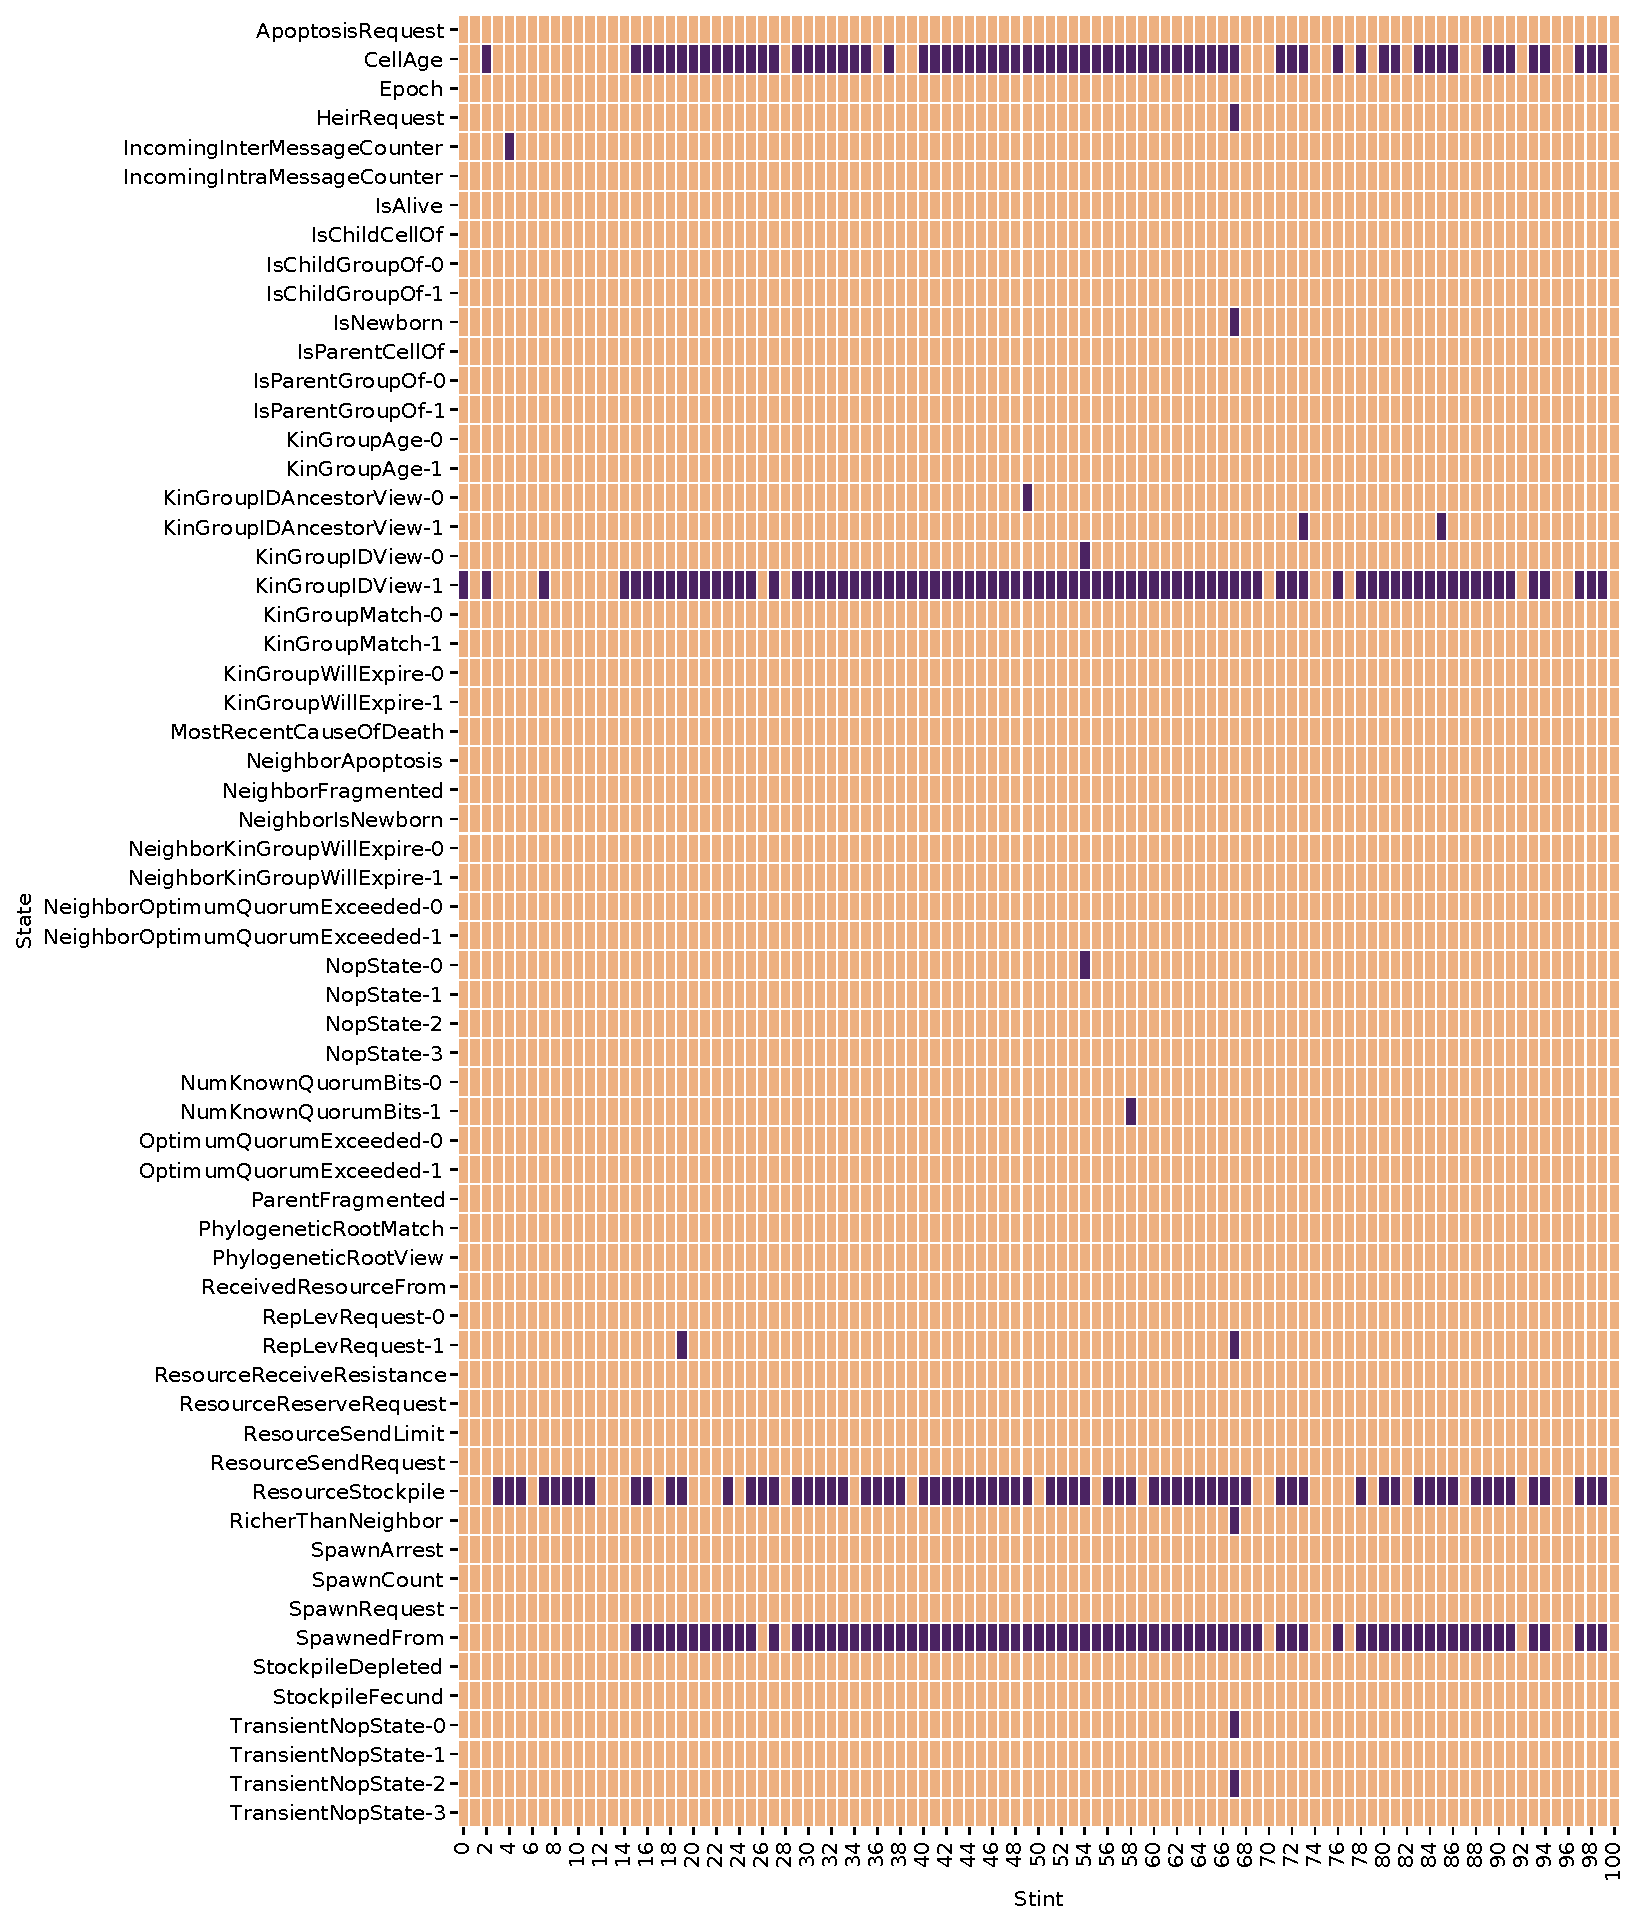
\includegraphics[width=\linewidth]{{plots/extrospective_perturbation/bucket=prq49+endeavor=16+transform=filter-Series-16005+val=extrospective-perturbation-fitness+viz=tall-heatmap+x=Stint+y=State+ext=}}

\caption{
Fitness effect of extrospective states (read-only state information of neighboring cells) for focal strains between stint 0 and 100.
Peach color indicates no fitness effect.
Burgundy indicates a significant fitness effect.
Supplementary material provides a description for each state.
}
\label{fig:extrospective_perturbation}
\end{figure*}

\begin{figure*}

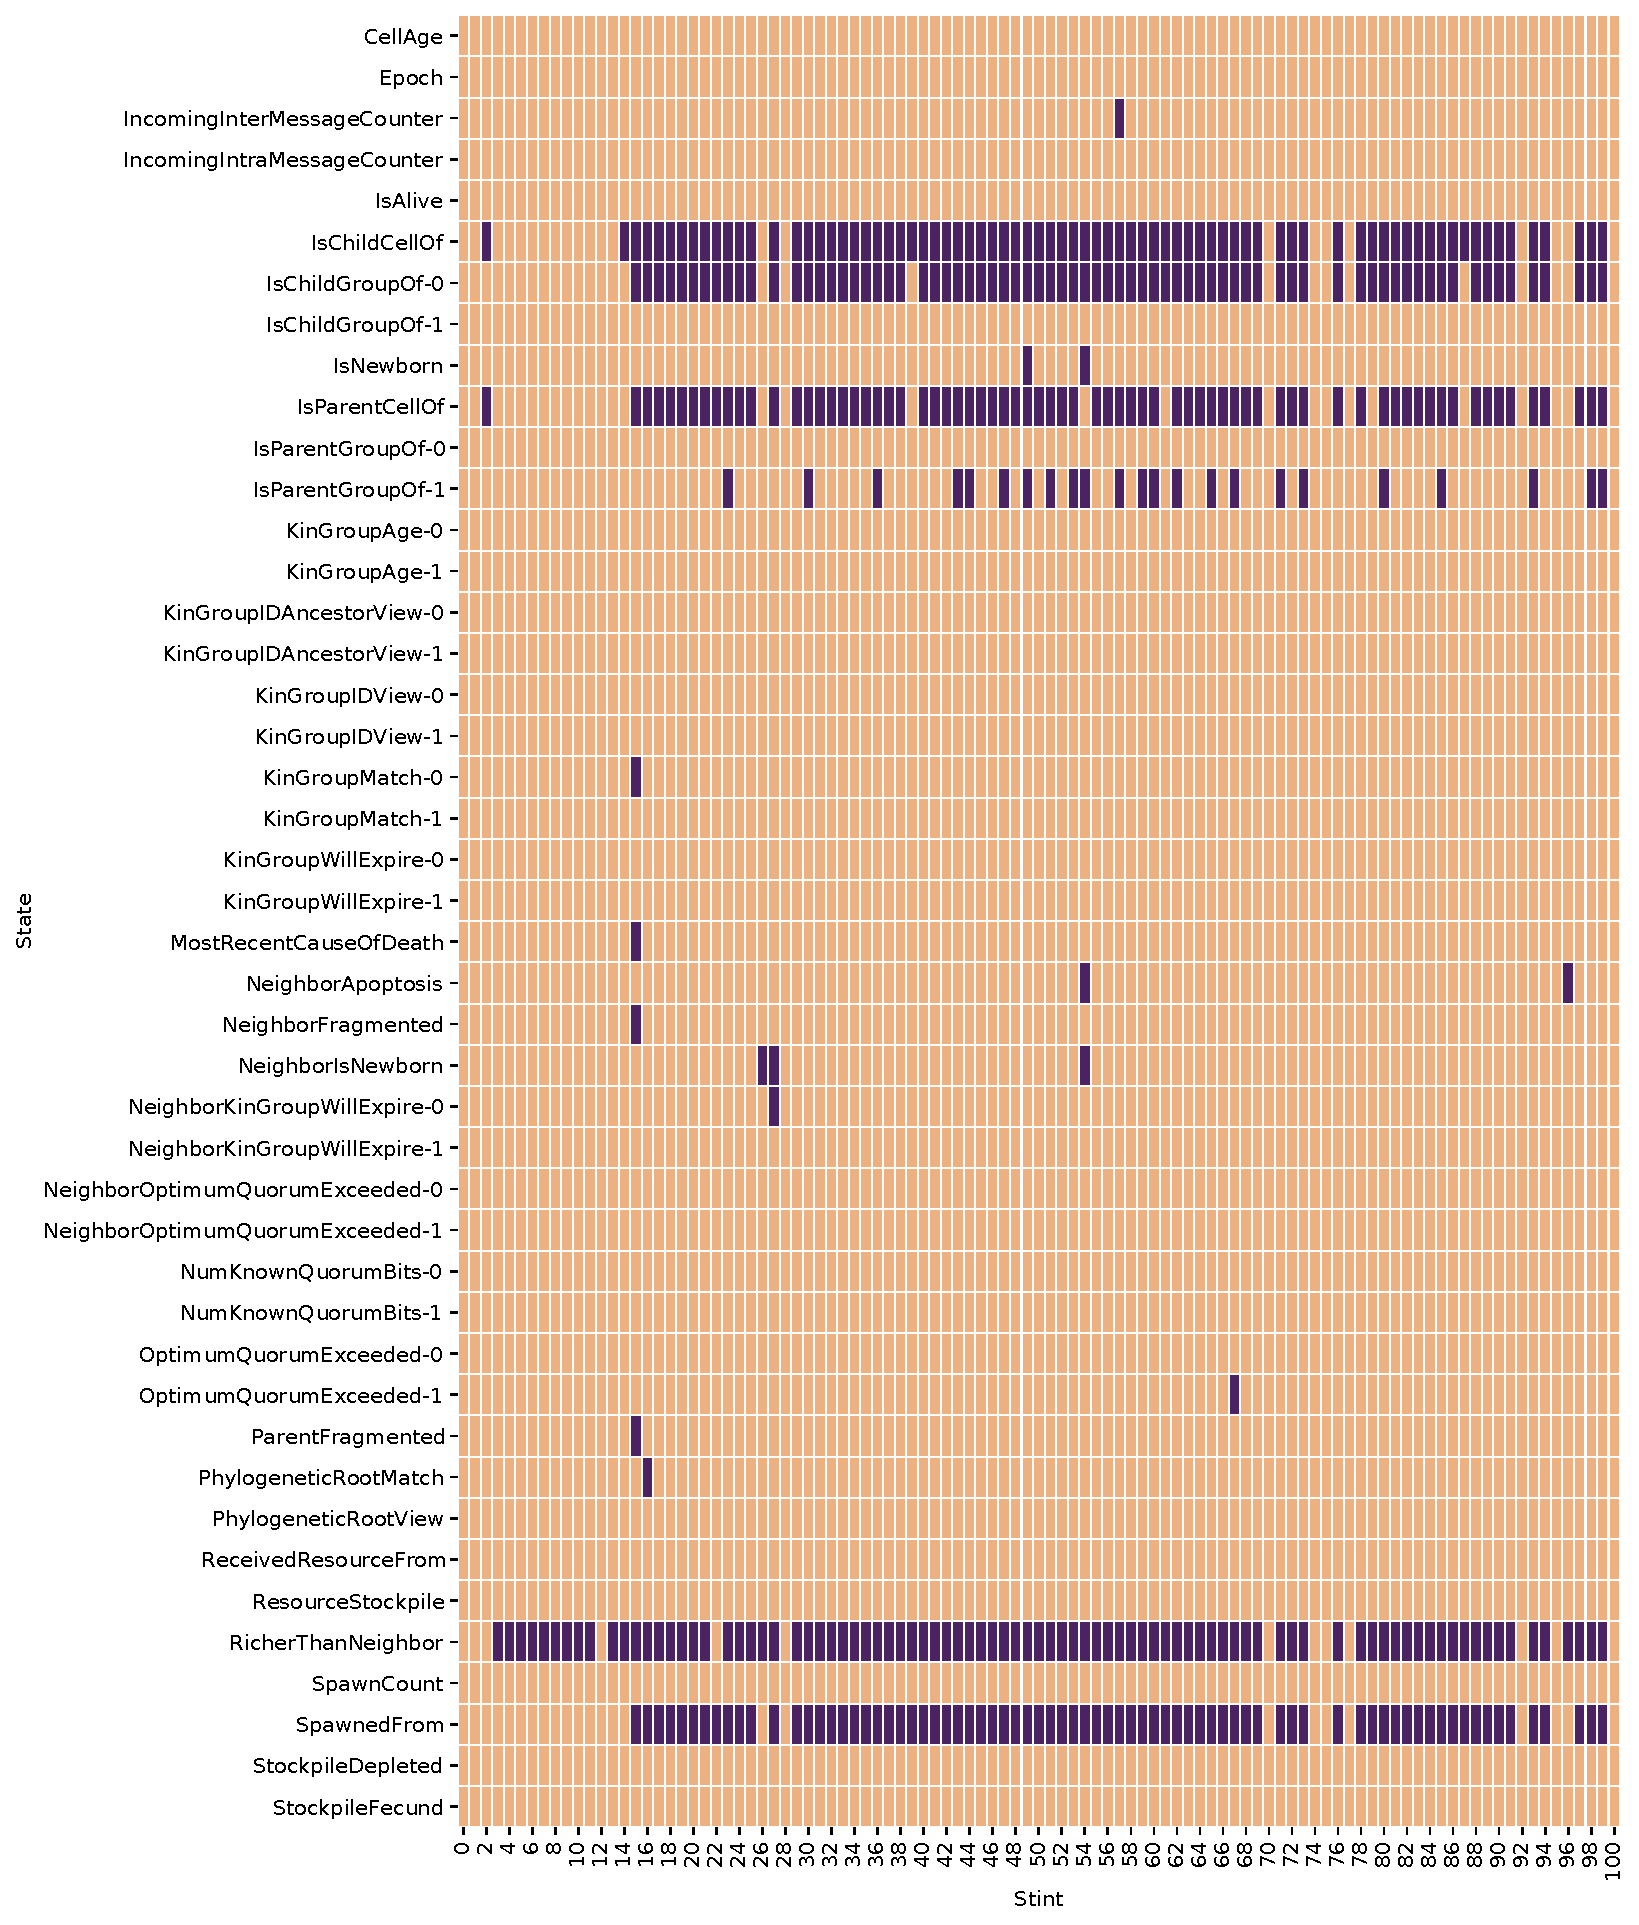
\includegraphics[width=\linewidth]{{plots/introspective_perturbation/bucket=prq49+endeavor=16+transform=filter-Series-16005+val=introspective-perturbation-fitness+viz=tall-heatmap+x=Stint+y=State+ext=}}

\caption{ Fitness effect of introspective states (state information of neighboring cells) for focal strains between stint 0 and 100.
Peach color indicates no fitness effect.
Burgundy indicates a significant fitness effect.
Supplementary material provides a description for each state. }
\label{fig:introspective_perturbation}
\end{figure*}


\begin{figure*}

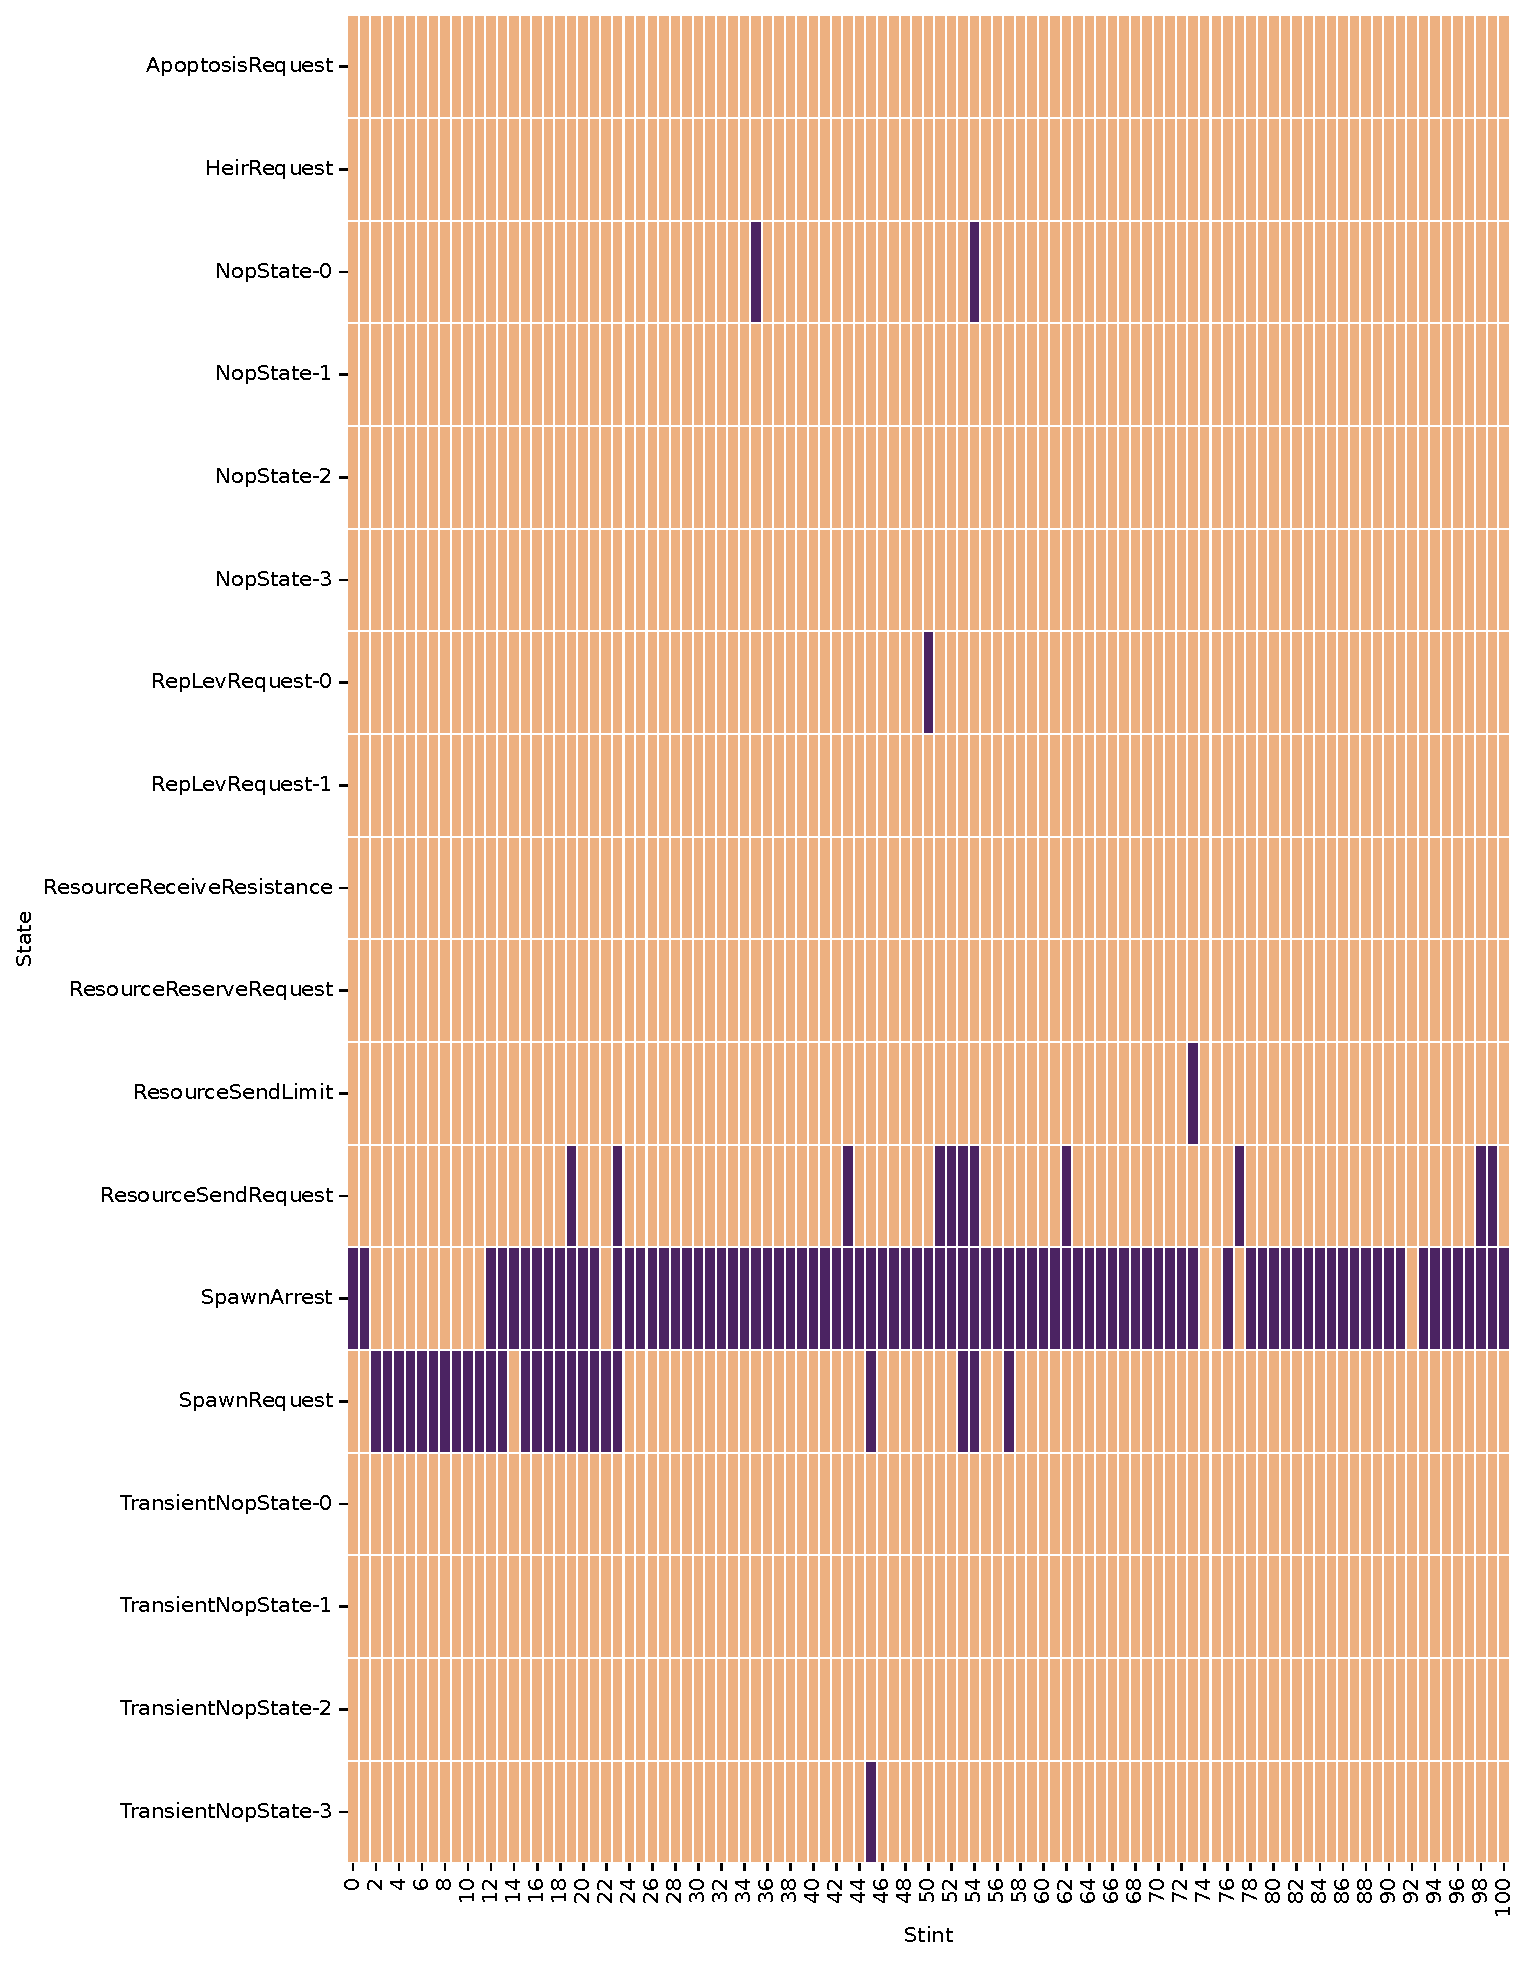
\includegraphics[width=\linewidth]{{plots/writable_perturbation/bucket=prq49+endeavor=16+transform=filter-Series-16005+val=writable-perturbation-fitness+viz=tall-heatmap+x=Stint+y=State+ext=}}

\caption{ Fitness effect of writable states (state information of neighboring cells) for focal strains between stint 0 and 100.
Peach color indicates no fitness effect.
Burgundy indicates a significant fitness effect.
Supplementary material provides a description for each state. }
\label{fig:writable_perturbation}
\end{figure*}



% \subsection{Phenotype Complexity}

% \begin{figure}

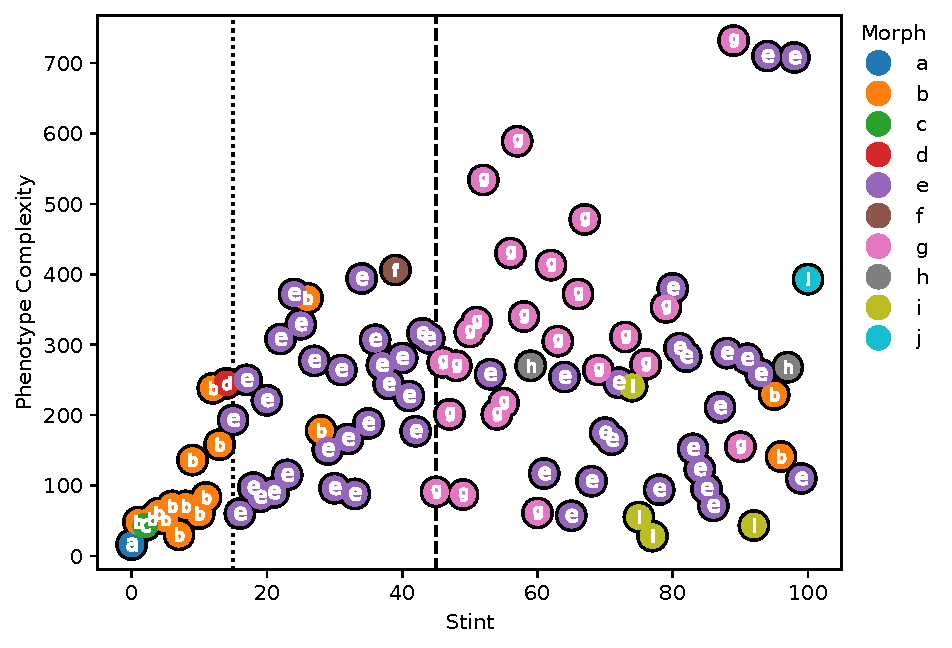
\includegraphics[width=\linewidth]{{plots/phenotype_complexity/bucket=prq49+cat=morph+endeavor=16+transform=filter-Series-16005+viz=letterscatter-vline+x=stint+y=phenotype-complexity+ext=}}

\caption{ Number of genome sites that contribute to phenotpe, measured as number sites remaining after phenotype-neutral nopout.
Color coding and letters correspond to qualitative morph codes described in Table \ref{tab:morph_descriptions}.
Dotted vertical line denotes emergence of morph $e$.
Dashed vertical line denotes emergence of morph $g$.
}
\label{fig:phenotype_complexity}
\end{figure}


% Phenotype complexity was highly volatile, bouncing at times from between more than 500 to less than 100 --- as shown in Figure \ref{fig:phenotype_complexity}.
% The maximum observed phenotype complexity was 732 sites at stint 89.

In the following sections, $L$ refers to the number of hierarchical kin group levels defined for the simulation.
In this work, we use $L=2$.

\section{Virtual CPU} \label{sec:virtual_cpu}

Each cardinal processor hosts a signalgp-lite virtual CPU \citep{lalejini2018evolving,moreno2021signalgp}.
Each CPU can host up to 16 active virtual cores.
If additional cores are required after all 16 available are in use, the oldest active core is killed and replaced.
Each virtual core contains 8 virtual \texttt{float} registers.

Cores execute round-robin in quasi-parallel, with up to 8 instructions being executed on a single core before execution shifts to the next active core.

Like SignalGP, the signalgp-lite system uses tag-matching to determine which modules to activate in response to incoming signals from the environment, from other agents (i.e., messages), and from internal events (i.e., execution of \texttt{call} and \texttt{fork} instructions).

In the DISHTINY simulation, each CPU hosts two independent module-lookup data structures.
The first module-lookup data structure is used to activate modules in response to internally-generated signals, messages from other cardinal processors within the same cell, and environmental events;
this module-lookup data structure contains \textit{all} modules within the genetic program.
The second module-lookup data structure is used to activate modules in response to messages from other cells;
this module-lookup data structure contains only modules with bitstring tags that end in 0.
(Hence, the subset of modules with bitstring tags that end in 1 \textit{cannot} be activated by messages from other cells, so that sensitive functionality like resource sharing and apoptosis can be protected from potentially malicious exploitation.)

We also use a tag-matching system to route \texttt{jump} instructions executed within a module.
When a module is loaded, all \texttt{local anchor} instructions are registered within a tag-matching data structure.
The local \texttt{jump} instruction routes to the best-matching local anchor.
If no matching local anchor is available, then no jump is performed and execution continues as if a \texttt{nop} instruction had elapsed.

\section{Tag Matching}

We use 64-bit bitstring tags to label modules and jump destinations.
We use a variant of Downing's streak metric to compute tag matches \citep{downing2015intelligence,moreno2023matchmaker}.
We deterministically select the single best-matching result for a tag lookup.
If there is a tie, an arbitrary result is selected.
For module-lookup, the best-matching tag must have a match quality at the 80th or better percentile among match qualities of pairs of randomly generated tags.
Otherwise, no module is activated.
For jump-lookup, the best match must be at the 50th or better percentile.
Otherwise, no jump is performed.

\section{Program Generation and Mutation}

Initial populations were seeded with programs consisting of 128 randomly generated instructions.
Program length was capped at 4096 instructions.

Mutation was applied to one in 10 reproductions where any kin group commonality was maintained and to 10 in 10 reproductions where it was not.
If mutation occurred, bits in the binary representation of the genome were flipped with 0.02\% probability.
If mutation occurred, sequence mutations were also introduced into the program at a per-site rate of 0.1\%.
Half of sequence mutations were deletion events, with a number of sites deleted drawn uniformly between 0 and 8.
Half of sequence mutations were insertion events, with a number of sites inserted drawn uniformly between 0 and 8.
When sites were inserted, half of the time randomly-generated instructions were added and half of the time the preceding sequence of instructions was duplicated.
With 0.1\% probability a sequence mutation took on severe intensity, meaning that the number of sites inserted or deleted was drawn uniformly between 0 and program size rather than between 0 and 8.

\section{Cooperative Resource Collection}

In order to ensure kin group structure had functional ramifications, we based part of cell resource collection on the number of contiguous kin group members.
To do this, we needed an efficient distributed method to approximate kin group size.

Each cell held a 64-bit bitstring with one chosen bit fixed.
We estimated group size by counting the number of distinct set bits (out of 64 available slots) that were contained within a kin group.
We refer to this count of distinct set bits as a group's ``quorum count.''

At every update within each tile, the simulation system broadcasts all bits that were known to be set within that tile's kin group.
This broadcast was only sent to neighboring tiles that were part of the same kin group as the broadcasting tile.
Each tile tracked which neighbor it learned of each set bit from so that when tiles left the kin group their set bits could be forgotten from the bits known to be set within the kin group.

This scheme was replicated independently for each kin group level simulated.
For the lowest-level kin group, a different fixed bit was chosen independently for each tile.
Thus, the quorum count for these lowest-level kin groups was a function of the number of cells contained.
For the highest-level kin group, each tile's fixed bit was chosen as a deterministic function of its lowest-level kin group ID.
Thus, the quorum count for these highest-level kin groups was a function of the number of lowest-level kin groups contained.

To incentivize kin group formation and maintenance, we gave each cell a 0.02 resource bonus every four updates for each non-self quorum count.
This bonus saturated at the simulation-defined target quorum count.
For both the lowest- and highest-level kin groups we used a target quorum count of 12.
The source code controlling cooperative resource collection can be found at \url{https://github.com/mmore500/dishtiny/blob/prq49/include/dish2/services/CollectiveHarvestingService.hpp}.

In addition to this cooperative resource collection mechanism, cells enjoyed a continuous resource inflow of 0.02 units per update.
The source code controlling base resource inflow can be found at \url{https://github.com/mmore500/dishtiny/blob/master/include/dish2/services/ResourceHarvestingService.hpp}.

To penalize groups that expanded beyond the simulation-defined target quorum count, we decayed held resource by a multiplicative factor of $0.9995^{2^n}$, where $n$ is the excess quorum count beyond the simulation-defined target.
The source code controlling cooperative resource collection can be found at \url{https://github.com/mmore500/dishtiny/blob/prq49/include/dish2/services/CollectiveResourceDecayService.hpp}.

In addition to any decay due to group size, held resource decayed at a rate of 0.05\% per update.
Received resource was decayed 0.099975\% upon receipt.


\section{Simulation Details}
\label{sec:simulation-details}

% adapted from https://tex.stackexchange.com/a/61803
\newenvironment{leveldown}% Demote sectional commands
  {\let\section\subsection%
   \let\subsection\subsubsection%
   \let\subsubsection\paragraph%
   \let\paragraph\subparagraph%
   %\let\subparagraph\relax%
  }{}

\begin{leveldown}
\section{Events}

This section enumerates simulation-managed events that were dispatched on virtual CPUs.
In addition to a program, each genome contained an array of 64-bit tags --- one for each event.
When an event's criteria was met in the simulation, the genome's corresponding tag was used to dispatch a module in the program and launch a core executing that module.

All events are also exposed to the cell as a corresponding input sensor.
The state of the event (0 for false, 1 for true) is stored in the sensor prior to virtual CPU execution.
In fact, events are triggered based on the reading of the sensor register (not by re-reading the underlying simulation state).
This means that experimental perturbations that perturb sensor input also disrupted event-handling, allowing the state interface complexity metric to measure both event-driven and sensor-based behaviors.

The source code controlling events can be found at \url{https://github.com/mmore500/dishtiny/tree/prq49/include/dish2/events} and \url{https://github.com/mmore500/dishtiny/blob/prq49/include/dish2/services/InterpretedIntrospectiveStateRefreshService.hpp}.

\subsection{Always}

This event is always dispatched.

\subsection{Is Child Cell Of}

Is this cell a daughter cell of the cardinal's neighbor?
Triggered if this cell was spawned from the cardinal's neighbor and its cell is younger than the neighbor.

\subsection{Is Child Group Of (0 thru $L-1$)}

Is this cell's kin group a daughter group of the cardinal's neighbor cell's kin group?
Triggered if a cell's kin group ancestor ID(s) are equal to the cardinal's neighbor's current kin group ID(s).

\subsection{Is Newborn}

This event is dispatched once when a cell is first born.
Triggered if cell age is less than frequency at which events are launched.

\subsection{Is Parent Cell Of}

Is this cardinal's cell the parent cell of the cardinal's neighbor?
Triggered if neighbor was spawned from cell and cell age is greater than neighbor age.

\subsection{Kin Group Match (0 thru $L-1$)}

Is this cell part of the same kin group as the cardinal's neighbor?
Triggered if a cell's kin group ID(s) are equal to the cardinal's neighbors' current kin group ID(s).

\subsection{Kin Group Mismatch (0 thru $L-1$)}

Is this cell part of a different kin group from the cardinal's neighbor cell?
Triggered if a cell's kin group ID(s) are not equal to the cardinal's neighbors' current kin group ID(s).

\subsection{Kin Group will Expire (0 thru $L-1$)}

Triggered if kin group age is greater than 80\% of the kin group expiration duration.
(Depending on experiment configuration, the group may be force-fragmented after expiration.)

\subsection{Kin Group will not Expire (0 thru $L-1$)}

Triggered if kin group age is less than or equal to than 80\% of the kin group expiration duration.

\subsection{Neighbor Apoptosis}

Triggered if the most recent cell death in the cardinal's neighbor tile was apoptosis.

\subsection{Neighbor Fragmented}

Triggered if the most recent cell death in the cardinal's neighbor tile was fragmentation.

\subsection{Neighbor Is Alive}

Triggered if a cardinal's neighbor tile is occupied by a live cell.

\subsection{Neighbor Is Newborn}

Triggered once for each time a newborn spawns into the cardinal's neighboring tile.
Triggered if the cardinal's neighbor's age is less than the frequency at which events are launched.

\subsection{Neighbor Is Not Alive}

Triggered if the cardinal's neighboring tile is not occupied.

\subsection{Neighbor Kin Group Will Expire (0 thru $L-1$)}

Triggered if the cardinal's cell neighbor's kin group age is less than or equal to 80\% of the kin group expiration duration.

\subsection{Neighbor Optimum Quorum Exceeded}

Triggered if the cardinal's cell neighbor's number of known quorum bits exceed the target quorum count.

\subsection{Optimum Quorum Exceeded (0 thru $L-1$)}

Triggered if the cell's number of known quorum bits exceed the target quorum count.

\subsection{Optimum Quorum Not Exceeded (0 thru $L-1$)}

Triggered if the cell's number of known quorum bits is less than or equal to than the target quorum count.

\subsection{Parent Fragmented}

Triggered if a cell's parent died from fragmentation.
That is, if the last cause of death on the current tile was fragmentation.

\subsection{Phylogenetic Root Match}

Does this cell descend from the same originally-generated genome as its neighbor?
Triggered if a cardinal's cell's root ID is equal to that cardinal's neighbor cell's root ID.

\subsection{Phylogenetic Root Mismatch}

Does this cell and its neighbor descend from a different originally-generated genomes?
Triggered if a cardinal's cell's root ID is not equal to that cardinal's neighbor cell's Root ID.

\subsection{Poorer Than Neighbor}

Does this cell have less resource stockpiled than its neighbor?
Triggered if a cardinal's cell has less resource than that cardinal's neighbor cell.

\subsection{Received Resource From}

Triggered if a cardinal's cell has received resource from that cardinal's neighbor cell.

\subsection{Richer Than Neighbor}

Does this cell have more resource stockpiled than its neighbor?
Triggered if a cardinal's cell has more resource in its stockpile than that cardinal's neighbor cell.

\subsection{Stockpile Depleted}

Is this cell's stockpile empty?
Triggered if a cell's stockpile is less than twice the base harvest rate.

\subsection{Stockpile Fecund}

Does this cell have enough stockpiled resource to fund cellular reproduction?
Triggered if a cell's stockpile is greater than 1.0.

\section{Operations}

% create command to draw operation tables
\newcommand{\opdef}[2]{
    \begin{tabular}{|
        >{\columncolor[HTML]{C0C0C0}}l |l|}
        \hline
        Prevalence & #1 \\ \hline
        Num Args   & #2 \\ \hline
    \end{tabular}
}

This section overviews the operation library made available to evolving signalgp-lite genetic programs within the simulation.

Within the program section of each genome, each instruction contained 
\begin{itemize}
\item an op code, specifying which operation should be performed;
\item a 64-bit bitstring, used as a tag for operations that required tag-matching or as data for some configurable operations; and
\item three integer arguments, specifying which registers the operation should apply to (many operations do not use all arguments).
\end{itemize}

In the operation descriptions below, we refer to register access via to the $n$th argument as \texttt{reg[arg\_n]}.
Each core has its own eight \texttt{float} registers.
All core registers are zeroed out at core launch.

In order to prevent bread-and-butter operations like global anchors, local anchors, and terminals from being swamped out by large instruction set size, we manually defined increased ``prevalences'' for some instructions.
This prevalence increased the probability of the operation being selected under mutations and initial program generation.
Prevalence works like increasing the number of identical copies of the operation included in the operation library.
We provide the prevalence of each operation below.

See \url{https://github.com/mmore500/dishtiny/tree/prq49/include/dish2/operations} for the source code of DISHTINY-specific operations and \url{https://github.com/mmore500/signalgp-lite/tree/b6c437f44136651aa6f4051d84bc62a86c2afbbe/include/sgpl/operations} for the source code of generic operations.

Refer to Section \ref{sec:virtual_cpu} for details on the virtual CPU running these instructions.

\subsection{Fork If}

\opdef{1}{1}

If \texttt{reg[arg\_0]} is nonzero, registers a request to activate a new core with the module best-matching the current instruction's tag.
These fork requests are only handled when the current core terminates.
Each core may only register 3 fork requests.

\subsection{Nop, 0 RNG Touches}

\opdef{1}{0}

Performs no operation for one virtual CPU cycle.

\subsection{Nop, 1 RNG Touches}

\opdef{1}{0}

Performs no operation for one virtual CPU cycle, and advances the RNG engine once.
(Important to nop-out operations that perform one RNG touch without causing side effects.)

\subsection{Nop, 2 RNG Touches}

\opdef{1}{1}

Performs no operation for one virtual CPU cycle, and advances the RNG engine twice.
(Important to nop-out operations that perform two RNG touches without causing side effects.)

\subsection{Terminate If}

\opdef{1}{1}

Terminates current core if \texttt{reg[arg\_0]} is nonzero.

\subsection{Add}

\opdef{1}{3}

Adds \texttt{reg[arg\_1]} to \texttt{reg[arg\_2]} and stores the result in \texttt{reg[arg\_0]}.

\subsection{Divide}

\opdef{1}{3}

Divides \texttt{reg[arg\_1]} by \texttt{reg[arg\_2]} and stores the result in \texttt{reg[arg\_0]}.
Division by zero can result in an \texttt{Inf} or \texttt{NaN} value.

\subsection{Modulo}

\opdef{1}{3}

Calculates the modulus of \texttt{reg[arg\_1]} by \texttt{reg[arg\_2]} and stores the result in \texttt{reg[arg\_0]}.
Mod by zero can result in a \texttt{NaN} value.

\subsection{Multiply}

\opdef{1}{3}

Multiplies \texttt{reg[arg\_1]} by \texttt{reg[arg\_2]} and stores the result in \texttt{reg[arg\_0]}.

\subsection{Subtract}

\opdef{1}{3}

Subtracts \texttt{reg[arg\_2]} from \texttt{reg[arg\_1]} and stores the result in \texttt{reg[arg\_0]}.

\subsection{Bitwise And}

\opdef{1}{3}

Performs a bitwise AND of \texttt{reg[arg\_1]} and \texttt{reg[arg\_2]} then stores the result in \texttt{reg[arg\_0]}.

\subsection{Bitwise Not}

\opdef{1}{2}

Computes the bitwise NOT of \texttt{reg[arg\_1]} and stores the result in \texttt{reg[arg\_0]}.

\subsection{Bitwise Or}

\opdef{1}{3}

Performs a bitwise OR of \texttt{reg[arg\_1]} and \texttt{reg[arg\_2]} then stores the result in \texttt{reg[arg\_0]}.

\subsection{Bitwise Shift}

\opdef{1}{3}

Shifts the bits of \texttt{reg[arg\_1]} by \texttt{reg[arg\_2]} positions.
(If \texttt{reg[arg\_2]} is negative, this is a right shift.
Otherwise it is a left shift.)
Stores the result in \texttt{reg[arg\_0]}.

\subsection{Bitwise Xor}

\opdef{1}{3}

Performs a bitwise XOR of \texttt{reg[arg\_1]} and \texttt{reg[arg\_2]} then stores the result in \texttt{reg[arg\_0]}.

\subsection{Count Ones}

\opdef{1}{2}

Counts the number of bits set in \texttt{reg[arg\_1]} and stores the result in \texttt{reg[arg\_0]}.

\subsection{Random Fill}

\opdef{1}{1}

Fills register pointed to by \texttt{reg[arg\_0]} with random bits chosen from a uniform distribution.

\subsection{Equal}

\opdef{1}{3}

Checks whether \texttt{reg[arg\_1]} is equal to \texttt{reg[arg\_2]} and stores the result in \texttt{reg[arg\_0]}.

\subsection{Greater Than}

\opdef{1}{3}

Checks whether \texttt{reg[arg\_1]} is greater than \texttt{reg[arg\_2]} and stores the result in \texttt{reg[arg\_0]}.

\subsection{Less Than}

\opdef{1}{3}

Checks whether \texttt{reg[arg\_1]} is less than \texttt{reg[arg\_2]} and stores the result in \texttt{reg[arg\_0]}.

\subsection{Logical And}

\opdef{1}{3}

Performs a logical AND of \texttt{reg[arg\_1]} and \texttt{reg[arg\_2]}, storing the result in \texttt{reg[arg\_0]}.

\subsection{Logical Or}

\opdef{1}{3}

Performs a logical OR of \texttt{reg[arg\_1]} and \texttt{reg[arg\_2]}, storing the result in \texttt{reg[arg\_0]}.

\subsection{Not Equal}

\opdef{1}{3}

Checks whether \texttt{reg[arg\_1]} is not equal to \texttt{reg[arg\_2]} and stores the result in \texttt{reg[arg\_0]}.

\subsection{Global Anchor} \label{sec:global_anchor}

\opdef{15}{0}

Marks a module-begin position.
Based on tag-lookup, new cores or global jump instructions may set the program counter to this instruction's program position.

This instruction can also mark a module-end position --- executing this instruction can terminate the executing core.
If no local anchor instruction is present between the current global anchor instruction and the preceding global anchor instruction, this operation will not terminate the executing core.
(This way, several global anchors may lead into the same module.)

However, if a local anchor instruction is present between the current global anchor instruction and the preceding global anchor instruction, this operation will terminate the executing core. 
Local jump instructions will only consider local anchors between the preceding global anchor and the subsequent global anchor instruction.

\subsection{Global Jump If}

\opdef{1}{2}

Jumps the current core to a global anchor that matches the instruction tag if \texttt{reg[arg\_0]} is nonzero.
If \texttt{reg[arg\_1]} is nonzero, resets registers.

\subsection{Global Jump If Not}

\opdef{1}{2}

Jumps the current core to a global anchor that matches the instruction tag if \texttt{reg[arg\_0]} is nonzero.
If \texttt{reg[arg\_1]} is zero, resets registers.

\subsection{Protected Regulator Adjust}

\opdef{1}{1}

Adjusts the regulator value of global jump table tags matching this instruction's tag by the amount \texttt{reg[arg\_0]}.

This regulator value affects the outcome of tag lookup for internal events and signals from the environment.
(Note, as described in \ref{sec:virtual_cpu}, that independent tag lookup tables handle activating genome modules across different contexts.)

\subsection{Protected Regulator Decay}

\opdef{1}{1}

Ages the regulator decay countdown of global jump table tags matching this instruction's tag by the amount \texttt{reg[arg\_0]}.
If \texttt{reg[arg\_0]} is negative, this can forestall decay. 

This decay countdown affects the outcome of tag lookup for internal events, and signals from the environment.
(Note, as described in \ref{sec:virtual_cpu}, that independent tag lookup tables handle activating genome modules across different contexts.)

\subsection{Protected Regulator Get}

\opdef{1}{1}

Gets the regulator value of the global jump table tag that best matches this instruction's tag.
Stores the value in \texttt{reg[arg\_0]}.

If no tag matches, a no-op is performed.

The regulator value gotten controls internal events and signals from the environment.
(Note, as described in \ref{sec:virtual_cpu}, that independent tag lookup tables handle activating genome modules across different contexts.)

\subsection{Protected Regulator Set}

\opdef{1}{1}

Sets the regulator value of global jump table tags matching this instruction's tag to \texttt{reg[arg\_0]}.

This regulator value affects the outcome of tag lookup for internal events and signals from the environment.
(Note, as described in \ref{sec:virtual_cpu}, that independent tag lookup tables handle activating genome modules across different contexts.)

\subsection{Local Anchor}

\opdef{20}{0}

Marks a program location local jump instructions may route to.
This program location is tagged with the instruction's tag.

As described in Section \ref{sec:global_anchor}, this operation also plays a role in determining whether global anchor instructions close a module.

\subsection{Local Jump If}

\opdef{1}{1}

Jumps to a local anchor that matches the instruction tag if \texttt{reg[arg\_0]} is nonzero.

\subsection{Local Jump If Not}

\opdef{1}{1}

Jumps to a local anchor that matches the instruction tag if \texttt{reg[arg\_0]} is zero.

\subsection{Local Regulator Adjust}

\opdef{1}{1}

Adjusts the regulator value of local jump table tags matching this instruction's tag by the amount \texttt{reg[arg\_0]}.

\subsection{Local Regulator Decay}

\opdef{1}{1}

Ages the regulator decay countdown of local jump table tags matching this instruction's tag by the amount \texttt{reg[arg\_0]}.
If \texttt{reg[arg\_0]} is negative, this can forestall decay.

\subsection{Local Regulator Get}

\opdef{1}{1}

Gets the regulator value of the local jump table tag that best matches this instruction's tag.
Stores the value in \texttt{reg[arg\_0]}.

If no tag matches, a no-op is performed.

\subsection{Local Regulator Set}

\opdef{1}{1}

Sets the regulator value of global jump table tags matching this instruction's tag to \texttt{reg[arg\_0]}.

\subsection{Decrement}

\opdef{1}{1}

Takes \texttt{reg[arg\_0]}, decrements it by one, and stores the result in \texttt{reg[arg\_0]}.

\subsection{Increment}

\opdef{1}{1}

Takes \texttt{reg[arg\_0]}, increments it by one, and stores the result in \texttt{reg[arg\_0]}.

\subsection{Negate}

\opdef{1}{1}

Negates \texttt{reg[arg\_0]} and stores the result in \texttt{reg[arg\_0]}.

\subsection{Not}

\opdef{1}{1}

Performs a logical not on \texttt{reg[arg\_0]} and stores the result in \texttt{reg[arg\_0]}.

\subsection{Random Bool}

\opdef{1}{1}

Stores \texttt{1.0f} to \texttt{reg[arg\_0]} with probability determined by this instruction's tag.
Otherwise, stores \texttt{0.0f} to \texttt{reg[arg\_0]}.

\subsection{Random Draw}

\opdef{1}{1}

Stores a randomly drawn float value to \texttt{reg[arg\_0]}.

\subsection{Terminal}

\opdef{50}{1}

Stores a genetically-encoded value to \texttt{reg[arg\_0]}.
This value is determined deterministically using the instruction's tag.

\subsection{Exposed Regulator Adjust}

\opdef{1}{1}

Adjusts the regulator value of global jump table tags matching this instruction's tag by the amount \texttt{reg[arg\_0]}.

This regulator value affects the outcome of tag lookup for messages from neighbor cells.
(Note, as described in \ref{sec:virtual_cpu}, that independent tag lookup tables handle activating genome modules across different contexts.)

\subsection{Exposed Regulator Decay}

\opdef{1}{1}

Ages the regulator decay countdown of global jump table tags matching this instruction's tag by the amount \texttt{reg[arg\_0]}.
If \texttt{reg[arg\_0]} is negative, this can forestall decay. 

This decay countdown affects the outcome of tag lookup for messages from neighbor cells.
(Note, as described in \ref{sec:virtual_cpu}, that independent tag lookup tables handle activating genome modules across different contexts.)

\subsection{Exposed Regulator Get}

\opdef{1}{1}

Gets the regulator value of the global jump table tag that best matches this instruction's tag.
Stores the value in \texttt{arg[0]}.

If no tag matches, a no-op is performed.

The regulator value gotten controls messages from other cells.
(Note, as described in \ref{sec:virtual_cpu}, that independent tag lookup tables handle activating genome modules across different contexts.)

\subsection{Exposed Regulator Set}

\opdef{1}{1}

Sets the regulator value of global jump table tags matching this instruction's tag to \texttt{reg[arg\_0]}.

This regulator value affects the outcome of tag lookup for messages from other cells.
(Note, as described in \ref{sec:virtual_cpu}, that independent tag lookup tables handle activating genome modules across different contexts.)

\subsection{Add to Own State}

\opdef{5}{1}

Adds \texttt{reg[arg\_0]} to the current value in a target writable state then stores the sum back in to that target writable state.

To determine the target writable state, interprets the first 32 bits of the instruction tag as an unsigned integer then calculates the remainder of integer division by the number of writable states.

\subsection{Broadcast Intra Message If}

\opdef{1}{1}

If \texttt{reg[arg\_0]} is nonzero, generates a message tagged with the instruction's tag that contains the core's current register state.
Broadcasts this message to every other cardinal within the cell.

\subsection{Multiply Own State}

\opdef{5}{1}

Multiplies \texttt{reg[arg\_0]} by the current value in a target writable state then stores the result back in to that target writable state.

To determine the target writable state, interprets the first 32 bits of the instruction tag as an unsigned integer then calculates the remainder of integer division by the number of writable states.

\subsection{Read Neighbor State}

\opdef{10}{1}

Reads a target readable state from the neighboring cell and stores it into \texttt{reg[arg\_0]}.

To determine the target readable state, interprets the first 32 bits of the instruction tag as an unsigned integer then calculates the remainder of integer division by the number of readable states.

\subsection{Read Own State}

\opdef{20}{1}

Reads a target readable state and stores it into \texttt{reg[arg\_0]}.

To determine the target readable state, interprets the first 32 bits of the instruction tag as an unsigned integer then calculates the remainder of integer division by the number of readable states.

\subsection{Send Inter Message If}

\opdef{5}{1}

If \texttt{reg[arg\_0]} is nonzero, generates a message tagged with the instruction's tag that contains the core's current register state.
Sends this message to the neighboring cell.

\subsection{Send Intra Message If}

\opdef{5}{1}

If \texttt{reg[arg\_0]} is nonzero, generates a message tagged with the instruction's tag that contains the core's current register state.
Sends this message to a target cardinal within the cell.

To determine the target cardinal, sums instruction arguments then calculates the remainder of integer division by the number of co-cardinals.

\subsection{Write Own State If}

\opdef{5}{2}

If \texttt{reg[arg\_1]} is nonzero, stores \texttt{reg[arg\_0]} into a target writable state.

To determine the target writable state, interprets the first 32 bits of the instruction tag as an unsigned integer then calculates the remainder of integer division by the number of writable states.

% create command to draw state tables
\newcommand{\instrospectivestatedef}[2]{
    \begin{tabular}{|
        >{\columncolor[HTML]{C0C0C0}}l |l|}
        \hline
        Type & #1 \\ \hline
        Category & #2 \\ \hline
    \end{tabular} \\
}

\section{Introspective State}

Introspective state refers to the collection of simulation-generated sensor values that evolving programs running within each cardinal processor can access via read-only operations.
Each cardinal processor has an independent copy of each piece of introspective state state.
(However, some introspective states representing cell state are set to identical values across cardinal processors within the same cell.)

Each cardinal processor's introspective state regularly copied and dispatched to that cardinal processor's neighbor cell, where it serves as read-only extrospective state.

Introspective state is organized into two categories:
\begin{enumerate}
    \item raw introspective state, and
    \item interpreted introspective state.
\end{enumerate}

Raw introspective state directly exposes aspects of simulation state.
Interpreted introspective state is filled with truthy values that are interpreted as booleans to dispatch environmentally-managed events.

See \url{https://github.com/mmore500/dishtiny/tree/prq49/include/dish2/peripheral/readable_state/introspective_state} for source code implementing introspective state.

\subsection{Is Child Cell Of}

\instrospectivestatedef{\texttt{char} (w/ boolean semantics)}{interpreted}

Did this cell spawn from this cardinal processor's neighbor cell?

\subsection{Is Child Group Of (0 thru $L-1$)}

\instrospectivestatedef{\texttt{char} (w/ boolean semantics)}{interpreted}

Does this cell's kin group ID descend directly from the neighbor's kin group ID?

\subsection{Is Newborn}

\instrospectivestatedef{\texttt{char} (w/ boolean semantics)}{interpreted}

Is this cell's age less than \texttt{EVENT\_LAUNCHING\_SERVICE\_FREQUENCY}?

\subsection{Is Parent Cell Of}

\instrospectivestatedef{\texttt{char} (w/ boolean semantics)}{interpreted}

Did this cardinal processor's neighbor cell spawn from this cell?
That is, was neighbor was spawned from this cell and is this cell older than neighbor?

\subsection{Is Parent Group Of}

\instrospectivestatedef{\texttt{char} (w/ boolean semantics)}{interpreted}

Did this cell's kin group descend directly from the cardinal processor's neighbor cell's kin group?
That is, is cell's kin group ancestor ID(s) equal to the cardinal processor's neighbor's current kin group ID(s).

\subsection{Kin Group Match (0 thru $L-1$)}

\instrospectivestatedef{\texttt{char} (w/ boolean semantics)}{interpreted}

Does this cell's kin group ID match the neighbor's kin group ID?

\subsection{Kin Group will Expire (0 thru $L-1$)}

\instrospectivestatedef{\texttt{char} (w/ boolean semantics)}{interpreted}

Is this cell's kin group age greater than 80\% of this level's \texttt{GROUP\_EXPIRATION\_DURATIONS}?

\subsection{Neighbor Apoptosis}

Was the neighbor tile's most recent death apoptosis?

\instrospectivestatedef{\texttt{char} (w/ boolean semantics)}{interpreted}

\subsection{Neighbor Fragmented}

Was group fragmentation the most recent cause of death in the cardinal processor's neighbor cell?

\instrospectivestatedef{\texttt{char} (w/ boolean semantics)}{interpreted}

\subsection{Neighbor Is Newborn}

\instrospectivestatedef{\texttt{char} (w/ boolean semantics)}{interpreted}

Is the neighbor's cell age less than \texttt{EVENT\_LAUNCHING\_SERVICE\_FREQUENCY}?

\subsection{Neighbor Kin Group Will Expire (0 thru $L-1$)}{interpreted}

\instrospectivestatedef{\texttt{char} (w/ boolean semantics)}{interpreted}

Is this cell's kin group age greater than 80\% of the this level's \texttt{GROUP\_EXPIRATION\_DURATIONS}?

\subsection{Neighbor Optimum Quorum Exceeded (0 thru $L-1$)}

\instrospectivestatedef{\texttt{char} (w/ boolean semantics)}{interpreted}

Is this cardinal processor's neighbor cell's kin group quorum count more than the simulation-defined target count \texttt{OPTIMAL\_QUORUM\_COUNT}?

\subsection{Optimum Quorum Exceeded (0 thru $L-1$)}

\instrospectivestatedef{\texttt{char} (w/ boolean semantics)}{interpreted}

Is this cell's kin group quorum count more than the simulation-defined target count \texttt{OPTIMAL\_QUORUM\_COUNT}?

\subsection{Parent Fragmented}

\instrospectivestatedef{\texttt{char} (w/ boolean semantics)}{interpreted}

Did the cell's parent die from fragmentation?
That is, was the last cause of death on the current tile was fragmentation?

\subsection{Phylogenetic Root Match}

\instrospectivestatedef{\texttt{char} (w/ boolean semantics)}{interpreted}

Does this cell's root ID equal the cardinal processor's cell neighbor's root ID?
(This means they originate from the same seed ancestor.)

\subsection{Richer Than Neighbor}

\instrospectivestatedef{\texttt{char} (w/ boolean semantics)}{interpreted}

Does this cell's stockpile more resource than the cardinal processor's cell neighbor?

\subsection{Stockpile Depleted}

\instrospectivestatedef{\texttt{char} (w/ boolean semantics)}{interpreted}

Is this cell's stockpile less than twice the base harvest rate?

\subsection{Stockpile Fecund}

\instrospectivestatedef{\texttt{char} (w/ boolean semantics)}{interpreted}

Does this cell have enough resource stockpiled to fund spawning an offspring cell?

\subsection{Cell Age}

\instrospectivestatedef{\texttt{size\_t}}{raw}

Number CellAgeService calls elapsed since cell was born.

\subsection{Epoch}

\instrospectivestatedef{\texttt{size\_t}}{raw}

Updates elapsed since start of simulation.

\subsection{Incoming Inter Message Counter}

\instrospectivestatedef{\texttt{size\_t}}{raw}

Counter tracking incoming messages from cardinal processor's neighbor cell.
Intermittently reset to zero.

\subsection{Incoming Intra Message Counter}

\instrospectivestatedef{\texttt{size\_t}}{raw}

Counter of incoming messages from other cardinal processors within the cell.
Intermittently reset to zero.

\subsection{Is Alive}

\instrospectivestatedef{\texttt{char} (w/ boolean semantics)}{raw}

Whether the cell is alive.
Although trivial as introspective state, this state is useful for neighbor cell's extrospective state.

\subsection{Kin Group Age ($0$ thru $L - 1$)}

\instrospectivestatedef{\texttt{size\_t}}{raw}

Number of epochs elapsed since kin group formation.

\subsection{Kin Group ID Ancestor View ($0$ thru $L - 1$)}

\instrospectivestatedef{\texttt{size\_t}}{raw}

Kin group ID from which cell's kin group ID is descended.

\subsection{Kin Group ID View ($0$ thru $L - 1$)}

\instrospectivestatedef{\texttt{size\_t}}{raw}

Kin group ID of this cell.

\subsection{Most Recent Cause of Death}{raw}

\instrospectivestatedef{\texttt{char}}{raw}

What was this the most recent cause of death on this tile?
Encoded using the \texttt{CauseOfDeath} enum.

\subsection{Num Known Quorum Bits (0 thru $L-1$)}

\instrospectivestatedef{\texttt{size\_t}}{raw}

What is this cell's known quorum count?
(How many unique quorum bits collected from kin group members are known?)

\subsection{Phylogenetic Root View}

\instrospectivestatedef{\texttt{size\_t}}{raw}

What is this cell's phylogenetic root ID?

(Which initially-generated ancestor is this cell descended from?)

\subsection{Received Resource From}

\instrospectivestatedef{\texttt{float}}{raw}

How much resource is being received from the cardinal processor's cell neighbor?

\subsection{Resource Stockpile}

\instrospectivestatedef{\texttt{float}}{raw}

Amount of resource this cell has.

\subsection{Spawn Count}

\instrospectivestatedef{\texttt{float}}{raw}

Number of offspring generated from this cell and sent to the cardinal processor's neighbor tile.
Includes offspring that do not successfully take into the neighbor tile or have not survived.

\subsection{Spawned From}

\instrospectivestatedef{\texttt{char} (w/ boolean semantics)}{raw}

Did this cell spawn from this cardinal processor's neighbor cell?

% create command to draw state tables
\newcommand{\writablestatedef}[2]{
    \begin{tabular}{|
        >{\columncolor[HTML]{C0C0C0}}l |l|}
        \hline
        Type & \texttt{#1} \\ \hline
    \end{tabular} \\
}

\section{Writable State}

Writable state refers to the collection of output values that evolving programs running within each cardinal can write to and read from.
Some of these outputs enable interaction with the simulation (i.e., control phenotypic characteristics).
Each cardinal has an independent copy of each piece of writable state state.

See \url{https://github.com/mmore500/dishtiny/tree/prq49/include/dish2/peripheral/readable_state/writable_state} for source code implementing writable state.

\subsection{Nop State ($4\times$)}

\writablestatedef{float}

Writing to this state has no external effect.
It can be used as global memory shared between cores.

\subsection{Transient Nop State ($4\times$)}

\writablestatedef{float}

Writing to this state has no external effect.
It is cleared regularly by the decay to baseline service.
It can be used as temporary global memory shared between cores.

\subsection{Apoptosis Request}

\writablestatedef{char}

Writing a nonzero value to this state causes cell death.

\subsection{Heir Request}

\writablestatedef{char}

If this state is set when cell death occurs, the cardinal's neighbor cell will inherit leftover resource from the cell's stockpile.

\subsection{RepLev Request (0 thru $L$)}

\writablestatedef{char}

Controls kin group inheritance for daughter cells spawned to this cardinal's neighbor tile.

If no copies of this state are set at cell spawn, the daughter cell will have no common kin group IDs.
If one copy of this state is set at cell spawn, the daughter cell will have one common kin group ID.
If $L$ copies of this state are set at cell spawn, the daughter cell will have $L$ common kin group IDs.

\subsection{Resource Receive Resistance}

\writablestatedef{float}

Setting this state reduces the amount of resource received from the cardinal's neighbor cell. 

\subsection{Resource Reserve Request}

\writablestatedef{float}

Setting this state prevents that amount of stockpiled resource from being drawn from to be sent to the cardinal's neighbor cell.

\subsection{Resource Send Limit}

\writablestatedef{float}

Setting this state caps the amount of resource that this cell can send to the cardinal's neighbor cell per update.

\subsection{Resource Send Request}

\writablestatedef{float}

Setting this state initiates resource sharing to the cardinal's neighbor cell.
The value stored controls the amount of resource shared.

\subsection{Spawn Arrest}

\writablestatedef{char}

Setting this state prevents this cell from spawning offspring into this cardinal's neighbor tile, even if sufficient resource is available.

\subsection{Spawn Request}

\writablestatedef{char}

Setting this state attempts to initiate spawning offspring into this cardinal's neighbor tile.
% create command to draw state tables
\newcommand{\cellsimservicedef}[2]{
    \begin{tabular}{|
        >{\columncolor[HTML]{C0C0C0}}l |l|}
        \hline
        Frequency & every #1 update(s) \\ \hline
    \end{tabular} \\
}

\section{Cellular Simulation Services}

Simulation logic is applied to each cell through a collection of distinct functors, referred to as services.

All services specified to run on a particular update are applied in sequence to a single cell.
(Some services run only every $n$th update.)
Then, to another randomly-chosen cell in a \texttt{thread\_local} population, and another until the entire population has been updated.

See \url{https://github.com/mmore500/dishtiny/tree/prq49/include/dish2/services} for source code implementing these services.

\subsection{Decay to Baseline Service}

\cellsimservicedef{32}

Decays a cell's global regulators, resets its controller-mapped peripheral states, and resets its transient NOP states.

\subsection{Running Log Purge Service}

\cellsimservicedef{64}

Purges a cell's running logs.
(Only affects data collection, not simulation logic.)

\subsection{Controller Mapped State Noise Service}

\cellsimservicedef{8}

Given a non-zero controller-mapped state defect rate, picks a random number $n$ from a Poisson distribution parameterized by \texttt{CONTROLLER\_MAPPED\_STATE\_DEFECT\_RATE}.
Then, it introduces $n$ defects to a cell's writable state.
Half of these defects zero out the state and half randomize it.

\subsection{Interpreted Introspective State Refresh Service}

\cellsimservicedef{i}

Refreshes the interpreted introspective state of a cell.

\subsection{Extrospective State Exchange Service}

\cellsimservicedef{1}

Used for experimental manipulations testing the fitness effect of extrospective state.
(Not part of core simulation logic.)

\subsection{Extrospective State Rotate Service}

\cellsimservicedef{1}

Used for experimental manipulations testing the fitness effect of extrospective state.
(Not part of core simulation logic.)

\subsection{Introspective State Exchange Service}

\cellsimservicedef{1}

Used for experimental manipulations testing the fitness effect of introspective state.
(Not part of core simulation logic.)

\subsection{Introspective State Rotate Service}

\cellsimservicedef{1}

Used for experimental manipulations testing the fitness effect of introspective state.
(Not part of core simulation logic.)

\subsection{CPU Execution Service}

\cellsimservicedef{1}

Executes a cell's genome on its cardinals processors for \texttt{HARDWARE\_EXECUTION\_CYCLES} virtual cycles.
The order of cardinal evaluation is randomized.
This is repeated \texttt{HARDWARE\_EXECUTION\_ROUNDS} times.

\subsection{Event Launching Service}

\cellsimservicedef{8}

Dispatches environmentally-managed events for each cardinal processor.

\subsection{Introspective State Rotate Restore Service}

\cellsimservicedef{1}

Used for experimental manipulations testing the fitness effect of introspective state.
(Not part of core simulation logic.)

\subsection{Introspective State Exchange Restore Service}

\cellsimservicedef{1}

Used for experimental manipulations testing the fitness effect of introspective state.
(Not part of core simulation logic.)

\subsection{Extrospective State Rotate Restore Service}

\cellsimservicedef{1}

Used for experimental manipulations testing the fitness effect of extrospective state.
(Not part of core simulation logic.)

\subsection{Extrospective State Exchange Restore Service}

\cellsimservicedef{1}

Used for experimental manipulations testing the fitness effect of extrospective state.
(Not part of core simulation logic.)

\subsection{Writable State Exchange Service}

\cellsimservicedef{1}

Used for experimental manipulations testing the fitness effect of writable state.
(Not part of core simulation logic.)

\subsection{Writable State Rotate Service}

\cellsimservicedef{1}

Used for experimental manipulations testing the fitness effect of writable state.
(Not part of core simulation logic.)

\subsection{Birth Setup Service}

\cellsimservicedef{16}

Births a new cell into the current cell.

This occurs by first iterating through the cell's cardinal processors' birth request inputs in random order.
While the cell's resource stockpile is greater than the \texttt{SPAWN\_DEFENSE\_COST}, the requests are ignored and the stockpile depleted by that cost.
The first request that cannot be defended against is then acted upon.
The current cell's death routine is called, the old genome is replaced by the incoming genome, and the cell's make-alive routine is called.

\subsection{Cell Age Service}

\cellsimservicedef{1}

Advances the cell age introspective state and refreshes kin group age introspective state.

\subsection{Collective Harvesting Service}

\cellsimservicedef{4}

Calculates the total amount of resource collectively harvested to this cell by the cell's kin group.
This amount increases with quorum count and saturates at \texttt{OPTIMAL\_QUORUM\_COUNT}.
Adds the harvested amount to the cell's resource stockpile.

\subsection{Collective Resource Decay Service}

\cellsimservicedef{1}

If the cell's quorum count exceeds \texttt{OPTIMAL\_QUORUM\_COUNT}, applies multiplicative decay to the cell's resource stockpile.
This effect strengthens exponentially with excess cell quorum count.

\subsection{Conduit Flush Service}

\cellsimservicedef{16}

Flushes each cardinal processors' inter-process and inter-thread output conduits.

\subsection{Inter Message Launching Service}

\cellsimservicedef{8}

Launches new virtual cores to process incoming inter-cell messages.

\subsection{Inter Message Purging Service}

\cellsimservicedef{8}

Purges excess incoming inter-cell messages that couldn't be handled due to virtual core availability.

\subsection{Intra Message Launching Service}

\cellsimservicedef{8}

Launches new virtual cores to process incoming messages from same-cell cardinal processors.

\subsection{Message Counter Clear Service}

\cellsimservicedef{16}

Intermittently resets introspective message count state.

\subsection{Quorum Service}

\cellsimservicedef{1}

Performs distributed estimation of kin group size by simulation.

Each cell has a single randomly-chosen index set within a fixed-length bitstring.
(Depending in parameter settings, some cells may have index set --- all positions within the bitstring are zeroed out.)

Broadcasts bits known to be set are to all neighbor cells within the same kin group.
Incoming bitstrings from neighbors are ORed with known bits.

The original neighbor each non-self bit was first learned from is recorded alongside that bit.
If that neighbor no longer broadcasts that bit, it is erased from the cell's known bits.

Updates latest quorum count into introspective state.

This scheme is replicated independently for each kin group level simulated.

\subsection{Resource Decay Service}

\cellsimservicedef{1}

Decays cell resource stockpile multiplicatively by \texttt{RESOURCE\_DECAY} constant.

\subsection{Resource Harvesting Service}

\cellsimservicedef{1}

Adds a constant amount to cell's resource stockpile.

\subsection{Resource Receiving Service}

\cellsimservicedef{4}

Calculates total amount of resource received across every cardinal processor, and then adds that total to resource stockpile.

If the cell is not alive, it instead refunds all received resources back to each sending cell.

\subsection{Resource Sending Service}

\cellsimservicedef{1}

Based on writable state within each cardinal processor, calculates and dispatches resource that should be shared to each neighbor cell.

\subsection{Spawn Sending Service}

\cellsimservicedef{16}

If available resource is greater than or equal to 1.0, iterates randomly through every cardinal processor to determine whether it requested to spawn and has not arrested spawning.
Then, one of these requests is dispatched at random and stockpile is decreased by one.

\subsection{State Input Jump Service}

\cellsimservicedef{8}

Pulls a fresh copy of each neighboring cardinal processor's current readable state.

\subsection{State Output Put Service}

\cellsimservicedef{8}

Dispatches a copy of each cardinal processor's current readable state to corresponding neighbor cells.

\subsection{Epoch Advance Service}

\cellsimservicedef{8}

The cell's current-known epoch count is advanced by one then set to the maximum of the cell's current-known epoch count and neighbor cells' current-known epoch count.

\subsection{Writable State Rotate Restore Service}

\cellsimservicedef{1}

Used for experimental manipulations testing the fitness effect of writable state.
(Not part of core simulation logic.)

\subsection{Writable State Exchange Restore Service}

\cellsimservicedef{1}

Used for experimental manipulations testing the fitness effect of writable state.
(Not part of core simulation logic.)

\subsection{Group Expiration Service}

\cellsimservicedef{64}

As group age exceeds \texttt{GROUP\_EXPIRATION\_DURATIONS}, with increasing probability fragments cell from its kin group.
This process kills the cell and replaces it in place with a daughter without kin ID commonality.

\subsection{Apoptosis Service}

\cellsimservicedef{16}

If any cardinal processors have requested apoptosis, do death routine on the cell.

% create command to draw state tables
\newcommand{\threadlocalsimservicedef}[2]{
    \begin{tabular}{|
        >{\columncolor[HTML]{C0C0C0}}l |l|}
        \hline
        Frequency & every #1 update(s) \\ \hline
    \end{tabular} \\
}

\section{Threadlocal Simulation Services}

Actions that are performed on each \texttt{thread\_local} population.

See \url{https://github.com/mmore500/dishtiny/tree/prq49/include/dish2/services_threadlocal} for source code implementing these services.

\subsection{Cell Update Service}

\threadlocalsimservicedef{1}

Performs each cell's simulation services, iterating over cells in randomized order.

\subsection{Diversity Maintenance Service}

\threadlocalsimservicedef{8}

Prevents any one originally-generated ancestor from sweeping the population, preserving deep phylogenetic diversity.

Counts cells that descend from each originally-seeded ancestor.
If more than \texttt{DIVERSITY\_MAINTENANCE\_PREVALENCE} of cells descend from a single seeded ancestor, decay their resource stockpiles.
The magnitude of this effect increases with excess prevalence.

\subsection{Stint Diversity Maintenance Service}

\threadlocalsimservicedef{n/a}

Prevents any one seeded or reconstituted stint-originating ancestor from sweeping the population, preserving phylogenetic diversity within a single stint.

Counts cells that descend from each seeded or reconstituted stint-originating ancestor.
If more than \texttt{STINT\_DIVERSITY\_MAINTENANCE\_PREVALENCE} of cells descend from a single seeded or reconstituted ancestor, decay their resource stockpiles.
The magnitude of this effect increases with excess prevalence.

\section{Runtime Parameters}

% create command to draw operation tables
\newcommand{\confdef}[2]{
    ~\\ \begin{tabular}{|
        >{\columncolor[HTML]{C0C0C0}}l |l|}
        \hline
        Type & \texttt{#1} \\ \hline
        Default   & \texttt{#2} \\ \hline
    \end{tabular}
}

This section enumerates simulation parameters and provides default settings that were used.

See \url{https://github.com/mmore500/dishtiny/blob/prq49/include/dish2/config/ConfigBase.hpp} for source code defining run time parameters.

Some parameter settings were overridden in some assays.
See \url{https://github.com/mmore500/dishtiny/tree/prq49/configpacks/bucket=prq49+diversity=0.50_series+mut_freq=1.00+mut_sever=1.00} for configuration files used in each assay and \url{https://github.com/mmore500/dishtiny/tree/prq49/slurm} for runscripts used in each assay.

\subsection{EXECUTION}

% start of EXECUTION

\subsubsection{N\_THREADS}

\confdef{size\_t}{4}

How many threads should we run with?

\subsubsection{RUN\_UPDATES}

\confdef{bool}{\texttt{false}}

Should we run evolution or skip directly to post-processing and data collection?

\subsubsection{RUN\_UPDATES}

\confdef{size\_t}{0}

How many updates should we run the experiment for?

\subsubsection{RUN\_SECONDS}

\confdef{double}{0}

How many updates should we run the experiment for?

\subsubsection{MAIN\_TIMEOUT\_SECONDS}

\confdef{double}{10800}

After how many seconds should we time out and fail with an error?

\subsubsection{END\_SNAPSHOT\_TIMEOUT\_SECONDS}

\confdef{double}{1200}

After how many seconds should the end snapshot timeout?

\subsubsection{LOG\_FREQ}

\confdef{double}{20}

How many seconds should pass between logging progress?

\subsubsection{ASYNCHRONOUS}

\confdef{size\_t}{3}

Should updates occur synchronously across threads and processes?

\subsubsection{SYNC\_FREQ\_MILLISECONDS}

\confdef{size\_t}{100}

How often updates occur synchronously across threads and processes for async mode 1?

\subsubsection{RNG\_PRESEED}

\confdef{utin64\_t}{std::numeric\_limits<uint64\_t>::max()}

Optionally override the calculated rng preseed.

\subsubsection{THROW\_ON\_EXTINCTION}

\confdef{bool}{true}

Should we throw an exception if populations go extinct?

% end of EXECUTION

\subsection{EXPERIMENT}

% start of EXPERIMENT

\subsubsection{RUN\_SLUG}

\confdef{std::string}{``default''}

Run-identifying slug.

\subsubsection{PHENOTYPIC\_DIVERGENCE\_N\_UPDATES}

\confdef{size\_t}{2048}

How many updates should we run phenotypic divergence experiments for?
If phenotypic divergence is not detected within this many updates, we consider two strains to be phenotypically identical.

\subsubsection{PHENOTYPIC\_DIVERGENCE\_N\_CELLS}

\confdef{size\_t}{100}

How many cells should we simulate while testing for phenotypic divergence?

\subsubsection{STINT}

\confdef{utin64\_t}{std::numeric\_limits<uint64\_t>::max()}

How many evolutionary stints have elapsed?

\subsubsection{SERIES}

\confdef{utin64\_t}{std::numeric\_limits<uint64\_t>::max()}

Which evolutionary series are we running?

\subsubsection{REPLICATE}

\confdef{std::string}{``''}

What replicate are we running?

\subsubsection{TREATMENT}

\confdef{std::string}{``none''}

What experimental treatment has been applied?

\subsubsection{SEED\_FILL\_FRACTION}

\confdef{double}{1.0}

If we are seeding the population, what fraction of available slots should we fill?

\subsubsection{GENESIS}

\confdef{std::string}{"generate"}

How should we initialize the population?
Can be ``generate'' to randomly generate a new population,  ``reconstitute'' to load a population from file, ``monoculture'' to load a single genome from file, or ``inoculate'' to load genomes annotated with root ID keyname attributes from file.

% end of EXPERIMENT

\subsection{DEMOGRAPHICS}

% start of DEMOCRAPHICS

\subsubsection{N\_CELLS}

\confdef{size\_t}{10000}

How many cells should be simulated?

\subsubsection{WEAK\_SCALING}

\confdef{bool}{false}

Should number of total cells be multiplied by the total number of threads (num procs times threads per proc)?

\subsubsection{N\_DIMS}

\confdef{size\_t}{DISH2\_NLEV}

What dimensionality should the toroidal mesh have?

\subsubsection{GROUP\_EXPIRATION\_DURATIONS}

\confdef{internal::nlev\_size\_t\_t}{internal::nlev\_size\_t\_t\{ 256, 1024 \}}

After how many \texttt{epochs} should groups stop collecting resource?

\subsubsection{CELL\_AGE\_DURATION}

\confdef{size\_t}{1024}

After how many epochs should cells die?

% end of DEMOGRAPHICS

\subsection{RESOURCE}

% start of RESOURCE

\subsubsection{MIN\_START\_RESOURCE}

\confdef{float}{0.8}

How much resource should a cell start with?

\subsubsection{MAX\_START\_RESOURCE}

\confdef{float}{0.9}

How much resource should a cell start with?

\subsubsection{RESOURCE\_DECAY}

\confdef{float}{0.995}

How much resource should remain each update?

\subsubsection{APOP\_RECOVERY\_FRAC}

\confdef{float}{0.8}

What fraction of \texttt{REP\_THRESH} is recovered to heirs after apoptosis?

\subsubsection{SPAWN\_DEFENSE\_COST}

\confdef{float}{1.1}

What is the cost of repelling an incoming spawn?

% end of RESOURCE

\subsection{HARVEST}

% start of HARVEST

\subsubsection{BASE\_HARVEST\_RATE}

\confdef{float}{0.02}

How much resource should cells accrue per update?

\subsubsection{COLLECTIVE\_HARVEST\_RATE}

\confdef{internal::nlev\_float\_t}{internal::nlev\_float\_t\{0.25\}}

How much resource should cells accrue per update?

\subsubsection{OPTIMAL\_QUORUM\_COUNT}

\confdef{internal::nlev\_float\_t}{internal::nlev\_size\_\_t\{12\}}

What group size does collective harvest work most effectively at?

% end of HARVEST

\subsection{QUORUM}

% start of QUORUM

\subsubsection{P\_SET\_QUORUM\_BIT}

\confdef{internal::nlev\_float\_t}{internal::nlev\_float\_t\{1.0\}}

What fraction of cells should have a quorum bit set?

% end of QUORUM

\subsection{GENOME}

\subsubsection{PROGRAM\_START\_SIZE}

\confdef{size\_t}{128}

How many instructions should initial programs be?

\subsubsection{PROGRAM\_MAX\_SIZE}

\confdef{size\_t}{4096}

How many instructions should programs be capped at?

\subsubsection{MUTATION\_RATE}

\confdef{internal::nlev\_float\_t}{internal::nreplev\_float\_t\{0.1\}}

For each replev, what fraction of cells should be mutated at all?

\subsubsection{POINT\_MUTATION\_RATE}

\confdef{float}{0.0002}

What fraction of bits should be scrambled?

\subsubsection{SEQUENCE\_DEFECT\_RATE}

\confdef{float}{0.001}

How often should sloppy copy defect occur?

\subsubsection{MINOR\_SEQUENCE\_MUTATION\_BOUND}

\confdef{size\_t}{8}

For minor sequence mutations, at most how many instructions should be inserted or deleted?

\subsubsection{SEVERE\_SEQUENCE\_MUTATION\_RATE}

\confdef{float}{0.001}

With what probability should sequence mutation be severe?

\subsection{HARDWARE}

\subsubsection{HARDWARE\_EXECUTION\_ROUNDS}

\confdef{size\_t}{1}

How many hardware cardinal rounds to run?

\subsubsection{HARDWARE\_EXECUTION\_CYCLES}

\confdef{size\_t}{16}

How many hardware cycles to run per round?

\subsubsection{CONTROLLER\_MAPPED\_STATE\_DEFECT\_RATE}

\confdef{float}{0.0005}

At what rate should bits should be flipped in writable memory?"

\subsection{SERVICES}

\subsubsection{APOPTOSIS\_SERVICE\_FREQUENCY}

\confdef{size\_t}{16}

Run service every ?? updates.
Must be a power of 2.

\subsubsection{BIRTH\_SETUP\_SERVICE\_FREQUENCY}

\confdef{size\_t}{16}

Run service every ?? updates.
Must be a power of 2.

\subsubsection{CONDUIT\_FLUSH\_SERVICE\_FREQUENCY}

\confdef{size\_t}{1}

Run service every ?? updates.
Must be a power of 2.

\subsubsection{COLLECTIVE\_HARVESTING\_SERVICE\_FREQUENCY}

\confdef{size\_t}{16}

Run service every ?? updates.
Must be a power of 2.

\subsubsection{CPU\_EXECUTION\_SERVICE\_FREQUENCY}

\confdef{size\_t}{4}

Run service every ?? updates.
Must be a power of 2.

\subsubsection{GROUP\_EXPIRATION\_SERVICE\_FREQUENCY}

\confdef{size\_t}{1}

Run service every ?? updates.
Must be a power of 2.

\subsubsection{RUNNING\_LOG\_PURGE\_SERVICE\_FREQUENCY}

\confdef{size\_t}{64}

Run service every ?? updates.
Must be a power of 2.

\subsubsection{DIVERSITY\_MAINTENANCE\_SERVICE\_FREQUENCY}

\confdef{size\_t}{64}

Run service every ?? updates.
Must be a power of 2.

\subsubsection{DIVERSITY\_MAINTENANCE\_PREVALENCE}

\confdef{double}{0.25}

If an originally-seeded ancestor's descendants constitute more than this fraction of the population, decay their resource stockpiles.

\subsubsection{STINT\_DIVERSITY\_MAINTENANCE\_SERVICE\_FREQUENCY}

\confdef{size\_t}{0}

Run service every ?? updates.
Must be a power of 2.

\subsubsection{STINT\_DIVERSITY\_MAINTENANCE\_PREVALENCE}

\confdef{double}{0.25}

If a seeded or reconstituted stint-originating ancestor's descendants constitute more than this fraction of the population, decay their resource stockpiles.

\subsubsection{DECAY\_TO\_BASELINE\_SERVICE\_FREQUENCY}

\confdef{size\_t}{32}

Run service every ?? updates.
                                                                                                        Must be a power of 2.

\subsubsection{EPOCH\_ADVANCE\_SERVICE\_FREQUENCY}

\confdef{size\_t}{8}

Run service every ?? updates.
Must be a power of 2.

\subsubsection{EVENT\_LAUNCHING\_SERVICE\_FREQUENCY}

\confdef{size\_t}{8}

Run service every ?? updates.
Must be a power of 2.
Must be > 1.

\subsubsection{INTERMITTENT\_CPU\_RESET\_SERVICE\_FREQUENCY}

\confdef{size\_t}{64}

Run service every ?? updates.
Must be a power of 2.

\subsubsection{INTERMITTENT\_STATE\_PERTURB\_SERVICES\_FREQUENCY}

\confdef{size\_t}{1}

Run service every ?? updates.
Must be a power of 2.

\subsubsection{INTER\_MESSAGE\_COUNTER\_CLEAR\_SERVICE\_FREQUENCY}

\confdef{size\_t}{16}

Run service every ?? updates.
Must be a power of 2.

\subsubsection{INTER\_MESSAGE\_LAUNCHING\_SERVICE\_FREQUENCY}

\confdef{size\_t}{8}

Run service every ?? updates.
Must be a power of 2.

\subsubsection{INTRA\_MESSAGE\_LAUNCHING\_SERVICE\_FREQUENCY}

\confdef{size\_t}{1}

Run service every ?? updates.
Must be a power of 2.

\subsubsection{STATE\_OUTPUT\_PUT\_SERVICE\_FREQUENCY}

\confdef{size\_t}{8}

Run service every ?? updates.
Must be a power of 2.

\subsubsection{PUSH\_SERVICE\_FREQUENCY}

\confdef{size\_t}{16}

Run service every ?? updates.
Must be a power of 2.

\subsubsection{QUORUM\_CAP\_SERVICE\_FREQUENCY}

\confdef{size\_t}{16}

Run service every ?? updates.
Must be a power of 2.

\subsubsection{QUORUM\_SERVICE\_FREQUENCY}

\confdef{size\_t}{1}

Run service every ?? updates.
Must be a power of 2.

\subsubsection{RESOURCE\_DECAY\_SERVICE\_FREQUENCY}

\confdef{size\_t}{1}

Run service every ?? updates.
Must be a power of 2.

\subsubsection{RESOURCE\_HARVESTING\_SERVICE\_FREQUENCY}

\confdef{size\_t}{1}

Run service every ?? updates.
Must be a power of 2.

\subsubsection{RESOURCE\_INPUT\_JUMP\_SERVICE\_FREQUENCY}

\confdef{size\_t}{1}

Run service every ?? updates.
Must be a power of 2.

\subsubsection{RESOURCE\_RECEIVING\_SERVICE\_FREQUENCY}

\confdef{size\_t}{4}

Run service every ?? updates.
Must be a power of 2.

\subsubsection{RESOURCE\_SENDING\_SERVICE\_FREQUENCY}

\confdef{size\_t}{1}

Run service every ?? updates.
Must be a power of 2.

\subsubsection{SPAWN\_SENDING\_SERVICE\_FREQUENCY}

\confdef{size\_t}{16}

Run service every ?? updates.
Must be a power of 2.

\subsubsection{STATE\_INPUT\_JUMP\_SERVICE\_FREQUENCY}

\confdef{size\_t}{8}

Run service every ?? updates.
Must be a power of 2.

\subsubsection{CONTROLLER\_MAPPED\_STATE\_NOISE\_SERVICE\_FREQUENCY}

\confdef{size\_t}{8}

Run service every ?? updates.
Must be a power of 2.

\subsection{DATA}

\subsubsection{PHENOTYPE\_EQUIVALENT\_NOPOUT}

\confdef{bool}{false}

Should we make and record a phenotype equivalent nopout strain at the end of the run? Must also enable ARTIFACTS\_DUMP.

\subsubsection{BATTLESHIP\_PHENOTYPE\_EQUIVALENT\_NOPOUT}

\confdef{bool}{false}

Should we make and record a phenotype equivalent nopout strain at the end of the run?
Must also enable ARTIFACTS\_DUMP.

\subsubsection{JENGA\_PHENOTYPE\_EQUIVALENT\_NOPOUT}

\confdef{bool}{false}

Should we make and record a phenotype equivalent nopout strain at the end of the run?
Must also enable ARTIFACTS\_DUMP.

\subsubsection{JENGA\_NOP\_OUT\_SAVE\_PROGRESS\_AND\_QUIT\_SECONDS}

\confdef{size\_t}{10800}

After how many seconds should we save nop-out progress and quit?

\subsubsection{TEST\_INTERROOT\_PHENOTYPE\_DIFFERENTIATION}

\confdef{bool}{false}

Should we test for phenotype differentiation between roots?

\subsubsection{ALL\_DRAWINGS\_WRITE}

\confdef{bool}{false}

Should we generate and record drawings of the final state of the simulation?
Must also enable DATA\_DUMP.

\subsubsection{DATA\_DUMP}

\confdef{bool}{false}

Should we record data on the final state of the simulation?

\subsubsection{RUNNINGLOGS\_DUMP}

\confdef{bool}{false}

Should we dump running logs at the end of the simulation?
Must also enable DATA\_DUMP.

\subsubsection{CENSUS\_WRITE}

\confdef{bool}{false}

Should we write the cell census at the end of the simulation?
Must also enable DATA\_DUMP.

\subsubsection{ARTIFACTS\_DUMP}

\confdef{bool}{false}

Should we record data on the final state of the simulation?

\subsubsection{BENCHMARKING\_DUMP}

\confdef{bool}{false}

Should we record data for benchmarking the simulation?

\subsubsection{ROOT\_ABUNDANCES\_FREQ}

\confdef{size\_t}{0}

How many updates should elapse between recording phylogenetic root abundances?
If 0, never record phylogenetic root abundances.
Must be power of two.

\subsubsection{ABORT\_IF\_COALESCENT\_FREQ}

\confdef{size\_t}{0}

How many updates should elapse between checking for coalescence? If 0, never check for coalescence.
Must be power of two.

\subsubsection{ABORT\_IF\_EXTINCT\_FREQ}

\confdef{size\_t}{0}

How many updates should elapse between checking for coalescence? If 0, never check for coalescence. Must be power of two.

\subsubsection{ABORT\_AT\_LIVE\_CELL\_FRACTION}

\confdef{double}{0.0}

Should we terminate once a live cell fraction is reached? If 0, will not terminate.

\subsubsection{REGULATION\_VIZ\_CLAMP}

\confdef{double}{10.0}

What bounds should we clamp regulation values into before running PCA visualization?

\subsubsection{RUNNING\_LOG\_DURATION}

\confdef{size\_t}{4}

How many purge epochs should we keep events in the running log?

\subsubsection{SELECTED\_DRAWINGS\_FREQ}

\confdef{size\_t}{0}

How many updates should elapse between outputting snapshot images?

\subsubsection{DRAWING\_WIDTH\_PX}

\confdef{double}{500.0}

What should the width of the drawings be, in pixels?

\subsubsection{DRAWING\_HEIGHT\_PX}

\confdef{double}{500.0}

What should the height of the drawings be, in pixels?

\subsubsection{SELECTED\_DRAWINGS}

\confdef{std::string}{``''}

What drawings should be drawn?
Provide slugified drawer names separated by colons.

\subsubsection{ANIMATE\_FRAMES}

\confdef{bool}{false}

Should we stitch the output images into a video?
Only valid if DRAWING\_FREQ is not 0.

\subsubsection{VIDEO\_FPS}

\confdef{size\_t}{16}

How many frames per second should the video be?

\subsubsection{VIDEO\_MAX\_FRAMES}

\confdef{size\_t}{960}

At most how many frames should output video include?

\section{Compile Time Parameters}

% create command to draw operation tables
\newcommand{\paramcompiletimedef}[2]{
    ~\\ \begin{tabularx}{\linewidth}{|
        >{\columncolor[HTML]{C0C0C0}}l |X|}
        \hline
        Type & \texttt{#1} \\ \hline
        Value   & \texttt{#2} \\ \hline
    \end{tabularx}
}

This section enumerates simulation parameters and provides default settings that were used.

See \url{https://github.com/mmore500/dishtiny/blob/prq49/include/dish2/spec/Spec_prq49.hpp} for source code defining compile time parameters.

\subsection{NLEV}

\paramcompiletimedef{size\_t}{2}

How many hierarchical kin group levels should be simulated?

\subsection{AMT\_NOP\_MEMORY}

\paramcompiletimedef{size\_t}{4}

How many nop and transient nop states should exist in the peripheral?

\subsection{STATE\_EXCHANGE\_CHAIN\_LENGTH}

\paramcompiletimedef{size\_t}{128}

How many callees should we displace state by in state exchange experiments?

\subsection{sgpl\_spec\_t::num\_cores}

\paramcompiletimedef{size\_t}{32}

How many virtual cores should each cardinal's virtual CPU be able to support?

\subsection{sgpl\_spec\_t::num\_fork\_requests}

\paramcompiletimedef{size\_t}{3}

How many fork requests can a virtual core make at most?

\subsection{sgpl\_spec\_t::num\_registers}

\paramcompiletimedef{size\_t}{8}

How many registers should each virtual core contain?

\subsection{sgpl\_spec\_t::switch\_steps}

\paramcompiletimedef{size\_t}{8}

Maximum num steps executed on one core before next core is executed.

\subsection{sgpl\_spec\_t::global\_matching\_t}

\paramcompiletimedef{typedef}{%
emp::MatchDepository<\newline
\hspace*{2em}// \mbox{program index type} \newline
\hspace*{2em}unsigned short, \newline
\hspace*{2em}// \mbox{match metric} \newline
\hspace*{2em}emp::OptimizedApproxDualStreakMetric<64>,\newline
\hspace*{2em}// \mbox{match selector} \newline\hspace*{2em}emp::statics::RankedSelector<\newline
\hspace*{4em}// \mbox{match threshold} \newline 
\hspace*{4em}std::ratio<1, 5>\newline
\hspace*{2em}>,\newline
\hspace*{2em}// \mbox{regulator} \newline
\hspace*{2em}emp::PlusCountdownRegulator<\newline
\hspace*{4em}std::deci, // Slope\newline
\hspace*{4em}std::ratio<1,4>, // MaxUpreg\newline
\hspace*{4em}std::deci, // ClampLeeway\newline
\hspace*{4em}2 // CountdownStart\newline
\hspace*{2em}>,\newline
\hspace*{2em}true, // raw caching \newline
\hspace*{2em}8 // regulated caching\newline
>
}

What matching datastructure implementation should we use for global jump tables?

\subsection{sgpl\_spec\_t::local\_matching\_t}

\paramcompiletimedef{typedef}{%
emp::MatchDepository<\newline
\hspace*{2em}// \mbox{program index type} \newline
\hspace*{2em}unsigned short, \newline
\hspace*{2em}// \mbox{match metric} \newline
\hspace*{2em}emp::OptimizedApproxDualStreakMetric<64>,\newline
\hspace*{2em}// \mbox{match selector} \newline\hspace*{2em}emp::statics::RankedSelector<\newline
\hspace*{4em}// \mbox{match threshold} \newline 
\hspace*{4em}std::ratio<1, 2>\newline
\hspace*{2em}>,\newline
\hspace*{2em}// \mbox{regulator} \newline
\hspace*{2em}emp::PlusCountdownRegulator<\newline
\hspace*{4em}std::deci, // Slope\newline
\hspace*{4em}std::ratio<1,4>, // MaxUpreg\newline
\hspace*{4em}std::deci, // ClampLeeway\newline
\hspace*{4em}2 // CountdownStart\newline
\hspace*{2em}>,\newline
\hspace*{2em}false, // raw caching \newline
\hspace*{2em}0 // regulated caching\newline
>
}

What matching datastructure implementation should we use for local jump tables?

\subsection{sgpl\_spec\_t::tag\_width}

\paramcompiletimedef{size\_t}{64}

Tag width in bits.
\end{leveldown}

% \clearpage
% \onecolumn

% \begin{lstlisting}[language=python, caption={Formula to calculate probability of deleterious outcome in nopout interpolation.}, label={lst:probability_deleterious}]
import math

def count_hands_with_k_or_more_sets(
    deck_size, hand_size, num_sets, set_size, k
):

    num_fixed = set_size * k
    deck_free = deck_size - num_fixed
    hand_free = hand_size - num_fixed

    if k > num_sets or k > hand_size or deck_free < 0 or hand_free < 0:
        return 0

    if set_size == 1:
        return sum(
            math.comb(num_sets, k_)
            * math.comb(deck_size - num_sets, hand_size - k_)
            for k_ in range(k, num_sets + 1)
            if hand_size >= k_
        )

    return (
        math.comb(deck_free, hand_free)
        * math.comb(num_sets, k)
    ) - count_hands_with_k_or_more_sets(
        deck_size,
        hand_size,
        num_sets,
        set_size,
        k=k+1,
    )
    
def probability_deleterious(
    n, h, m, s
):
    return count_hands_with_k_or_more_sets(
        n, h, m, s, 1
    ) / math.comb(n, h)

\end{lstlisting}


% \twocolumn

% \pragmaonce

% adapted from https://www.overleaf.com/learn/latex/Commands
\providecommand{\dissertationonly}[1]{%
% adapted from https://tex.stackexchange.com/a/33577
\ifdefined\DISSERTATION%
#1%
\else%
\fi
}


\section{Supplementary Figures}

\FloatBarrier

\dissertationonly{This section provides supplementary figures for Chapter \ref{ch:measuring-cna}.}

% \section{Phylogenetic Reconstruction}

Event tags were collected from a 102-stint run.
Each stint has 35 event tags.
They each have a xxxx point-mutation rate per generation, and thus a yyyy point-mutation rate per stint.
Tags from stints 101 and 102 were discarded as they are a side effect of xxx, and the run had already been concluded by then.

The point-mutation distance between tags was calculated using a pairwise Hamming metric.
These distances were stored as a matrix \ref{phylo_distance_matrix_heatmap}, along with the phenotype categories for each stint.

To generate the phylogenetic tree \ref{phylo_nj_tree}, the distance matrix was transformed to a lower-triangular matrix, and then generated using BioPython's \texttt{Bio.Phylo.TreeConstruction.DistanceMatrix()} constructor along with the Neighbor Joining clustering method.
The non-terminal branch lengths were adjusted to equal the average branch length of their children.
Terminal nodes were then sorted by time (lowest stint first) with respect to their sibling nodes.
Each parent of a subtree was then assigned the value of the lowest child and then also sorted across its siblings.\
This was repeated until reaching the root node.

The parsimony tree was built using BioPython's \texttt{Phylo.TreeConstruction.ParsimonyTreeConstructor}, using the default \texttt{Phylo.TreeConstruction.ParsimonyScorer} scorer along with the Nearest Neighbor Interchanges searcher.
In conformance to the \texttt{phylip} format, stint tags were 'aligned' by concatenation across stints, and stint IDs were padded up to length 10 with left-leading zeros.
The tree-finding algorithm was then executed until an optimal solution was found.
Since stints 0 and 1 are outliers, the parsimony tree was stored both with them and without them, rerooted at stint 2.

The SciPy linkage tree \ref{phylo_scipy_linkage_tree} was generated using SciPy's \texttt{scipy.cluster.hierarchy.linkage} function with default arguments.
This was then converted into a dendropy tree, which in turn was converted into an ALife dataframe.
The ALife dataframe was finally converted into a standard BioPython tree, which was then sorted using the sibling method, and stored.

All trees were drawn unsorted, sorted, and ladderized using BioPython's \texttt{ladderize} method.
These drawings were generated both with and without 'outlier' nodes (stints 0 and 1).

\begin{figure*}
\centering
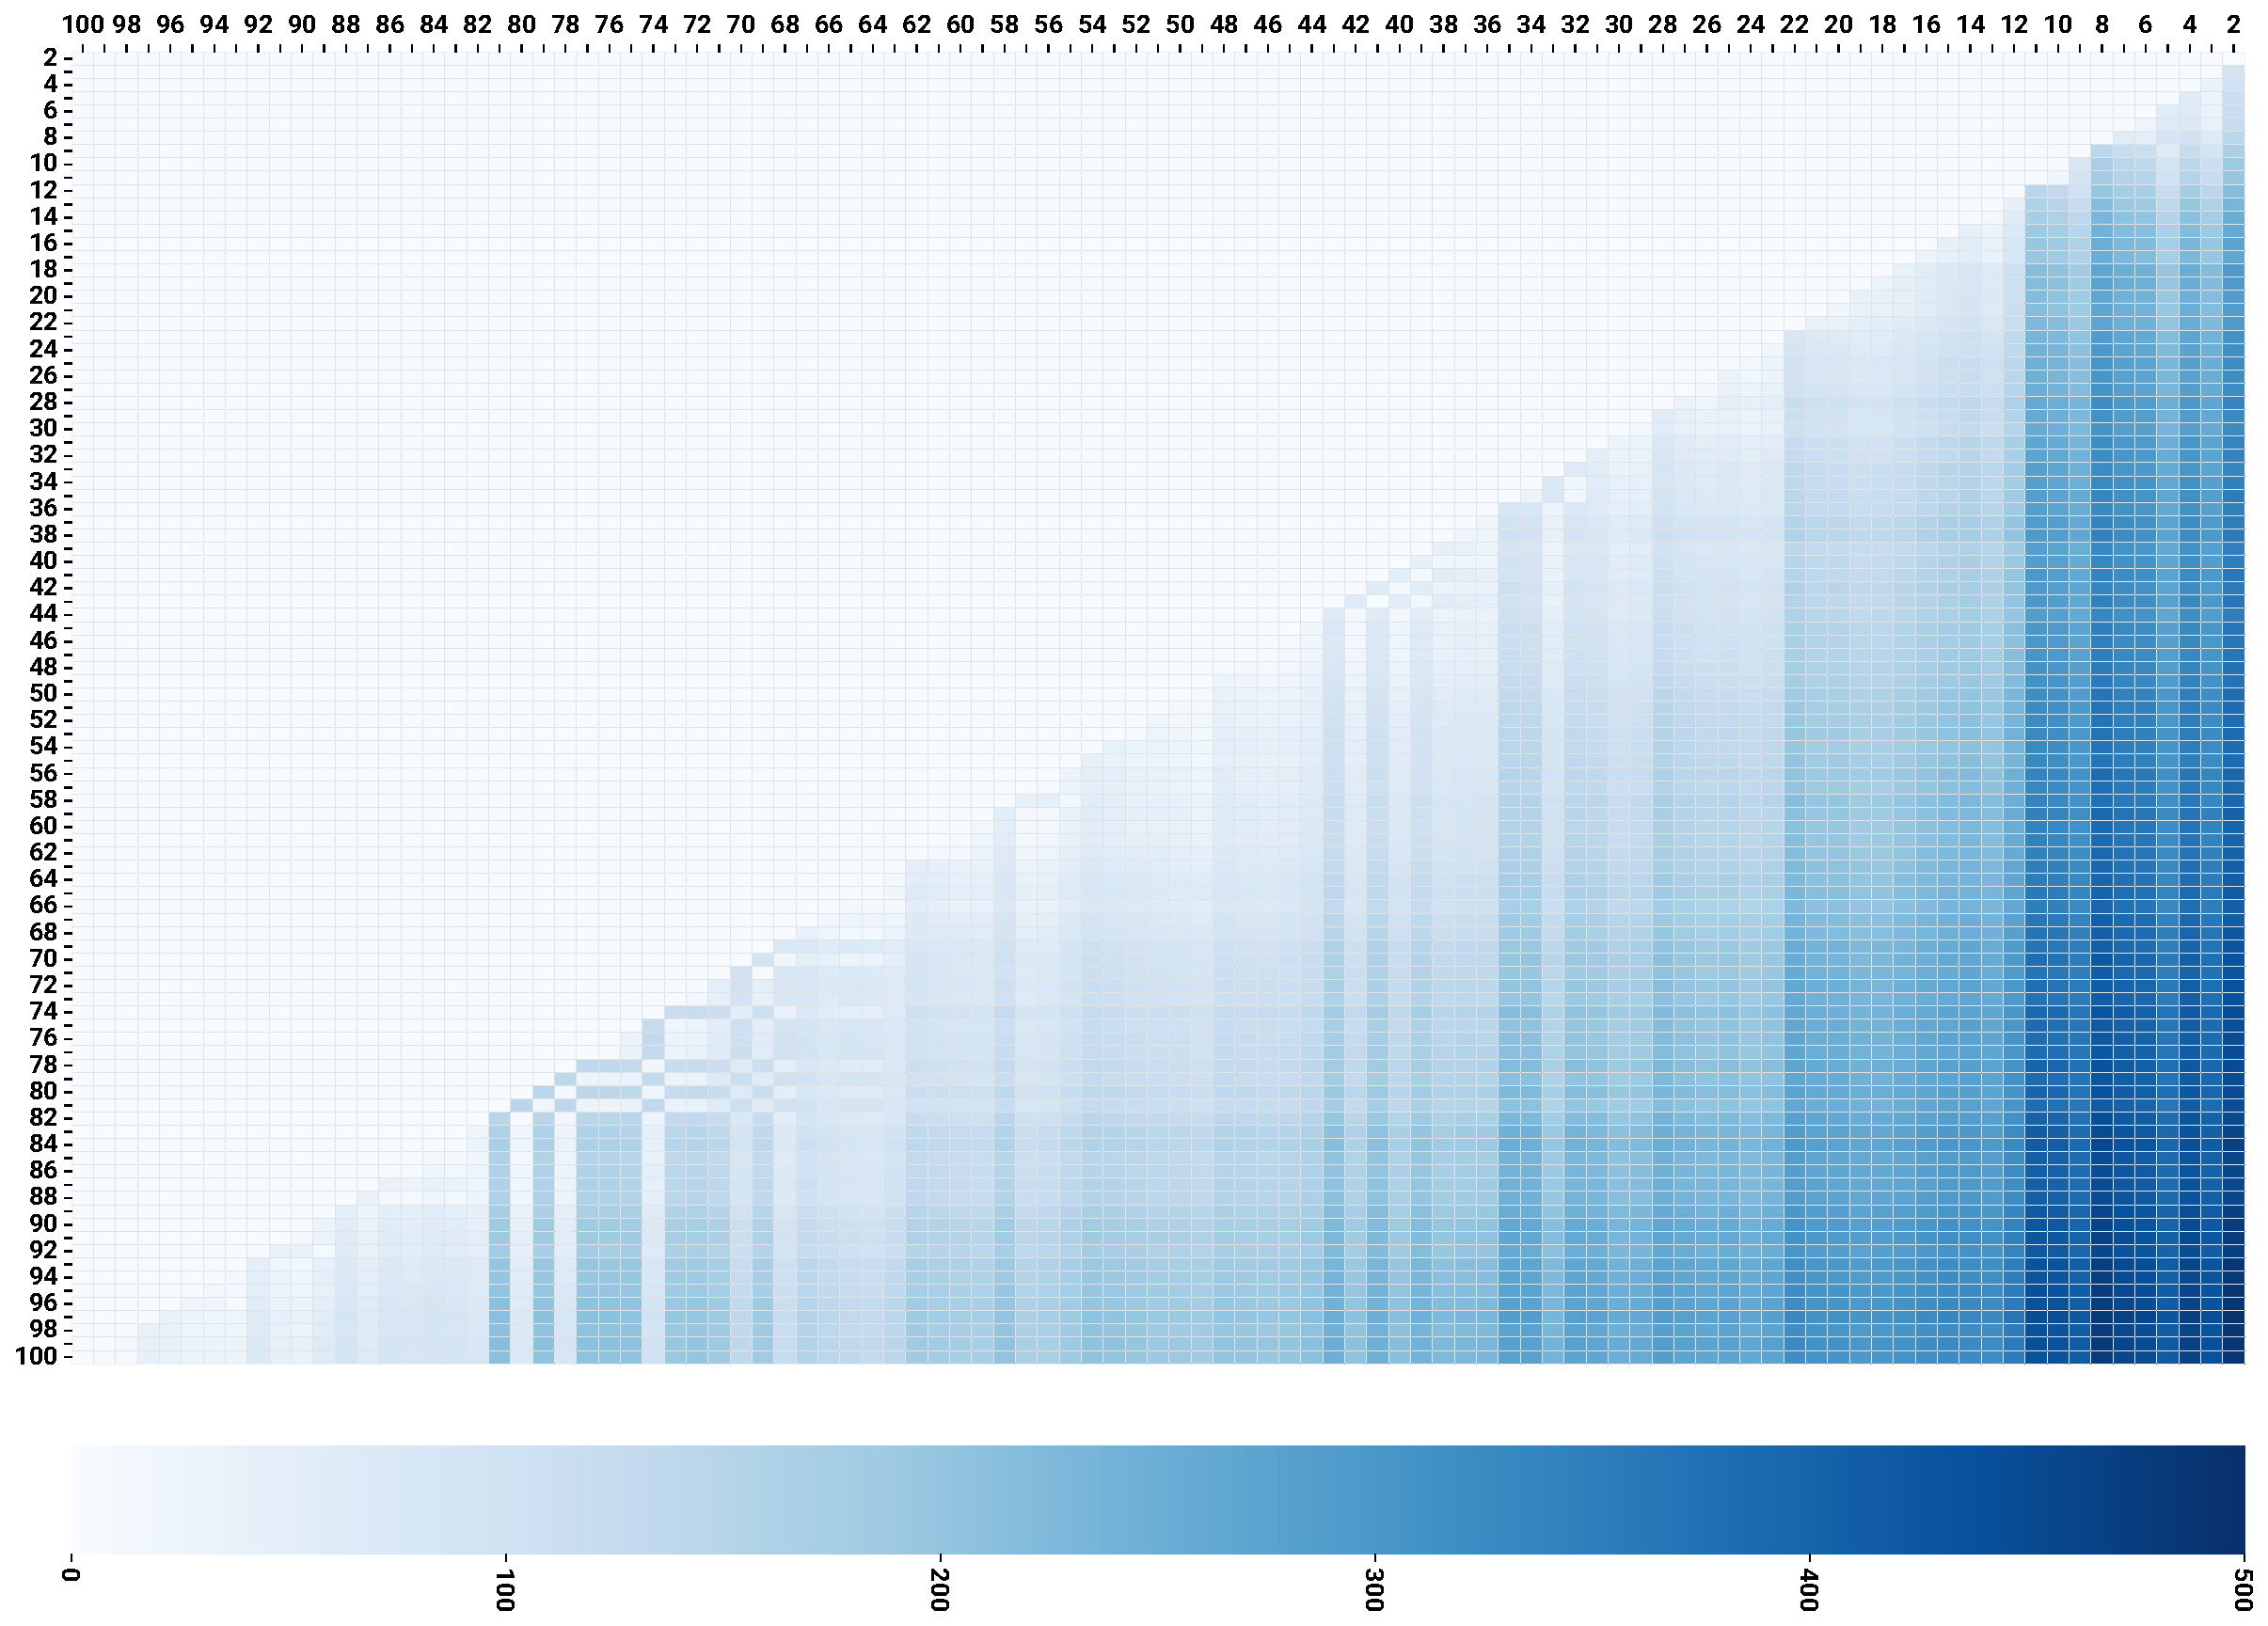
\includegraphics[width=0.8\linewidth]{{submodule/dishtiny_event_tag_phylogenetics/teeplots/distance_matrix_no_outliers/cmap=blues+linecolor=88888820+viz=heatmap+ext=}}

\caption{
TODO
}
\label{fig:phylo_distance_matrix_heatmap}
\end{figure*}



\begin{figure*}
\centering
\includegraphics[width=0.8\linewidth]{{submodule/dishtiny_event_tag_phylogenetics/teeplots/phylo_tree_no_outliers/viz=draw+ext=}}

\caption{
TODO
}
\label{fig:phylo_nj_tree}
\end{figure*}

\begin{figure*}
\centering
\includegraphics[width=0.8\linewidth]{{submodule/dishtiny_event_tag_phylogenetics/teeplots/scipy_linkage_tree_no_outliers/viz=draw+ext=}}

\caption{
Phylogeny of sampled focal strain representatives across stints reconstructed using hierarchical clustering algorithm \citep{virtanen2020scipy}.
Each leaf node corresponds to a sampled representative.
Representatives from stints 0 and 1, which share no common ancestry with representatives from other stints, are excluded.
Numbers refer to stint that each representative was sampled from.
Color coding and parentheticals of stint labels correspond to qualitative morph codes described in Table \ref{tab:morph_descriptions}.
}
\label{fig:phylo_scipy_linkage_tree}
\end{figure*}



% \begin{figure}

% \begin{subfigure}{0.5\textwidth}

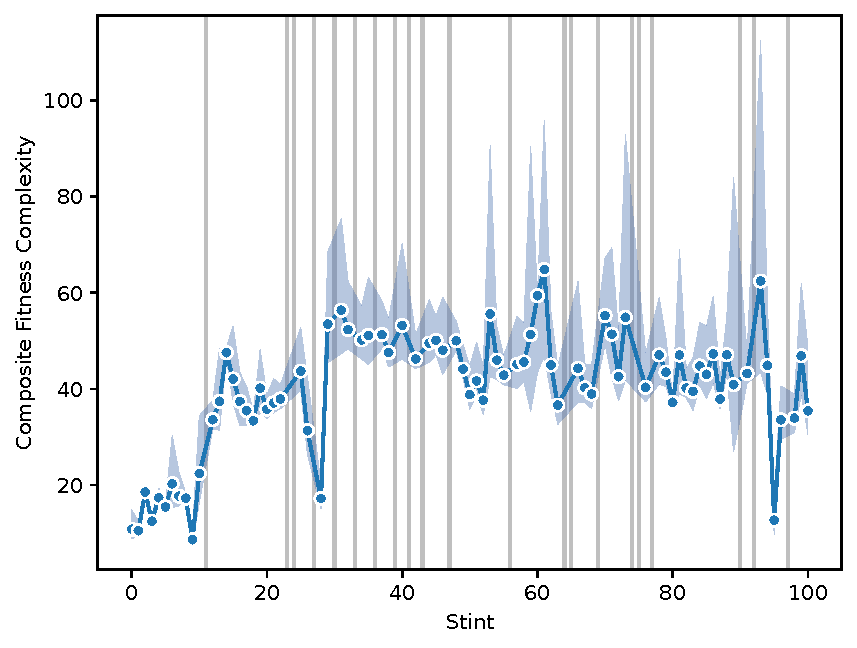
\includegraphics[width=\linewidth]{{plots/composite_fitness_complexity_alt/bucket=prq49+ci=95+endeavor=16+transform=filter-Series-16005+viz=scatter-err-vline+x=stint+y=composite-fitness-complexity+ext=}}

\caption{ Composite fitness complexity.
% An alternate rendering of Figure \ref{fig:fitness_complexity:composite_fitness_complexity}.
}
\label{fig:fitness_complexity_alt:composite_fitness_complexity_alt}

\end{subfigure}%

% \begin{subfigure}{0.5\textwidth}

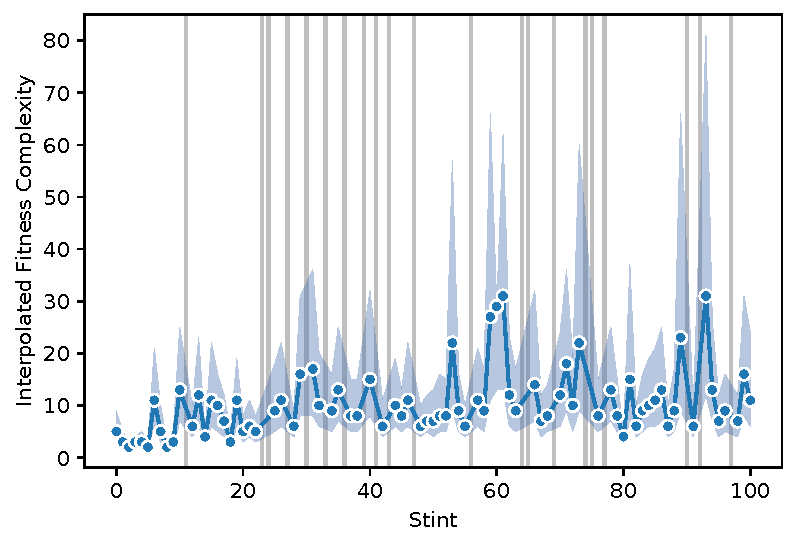
\includegraphics[width=\linewidth]{{plots/interpolated_fitness_complexity_alt/bucket=prq49+endeavor=16+transform=filter-Series-16005+viz=scatter-err-vline+x=stint+y=interpolated-fitness-complexity+ext=}}

\caption{ Interpolated fitness complexity. 
% An alternate rendering of Figure \ref{fig:fitness_complexity:interpolated_fitness_complexity}.
}
\label{fig:fitness_complexity_alt:interpolated_fitness_complexity_alt}

\end{subfigure}%

\caption{
Stub of content removed from supplement.
Left in to maintain figure numbering.
% Alternate renderings of Figure \ref{fig:fitness_complexity}.
}
\label{fig:fitness_complexity_alt}

\end{figure}

\begin{figure*}

\begin{subfigure}{0.5\textwidth}

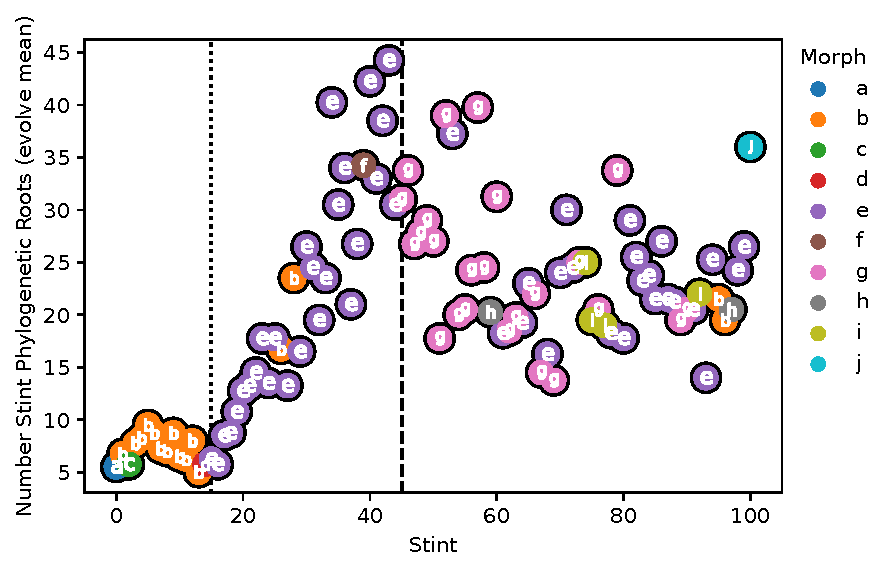
\includegraphics[width=\linewidth]{{plots/phylogeny/bucket=prq49+cat=morph+endeavor=16+transform=filter-Series-16005+viz=letterscatter-vline+x=stint+y=number-stint-phylogenetic-roots-evolve-mean+ext=}}

\caption{
Number of genomes from the beginning of a stint with extant offspring at the end of that stint. 
}
\label{fig:phylogeny:stint_roots}

\end{subfigure}%
\begin{subfigure}{0.5\textwidth}

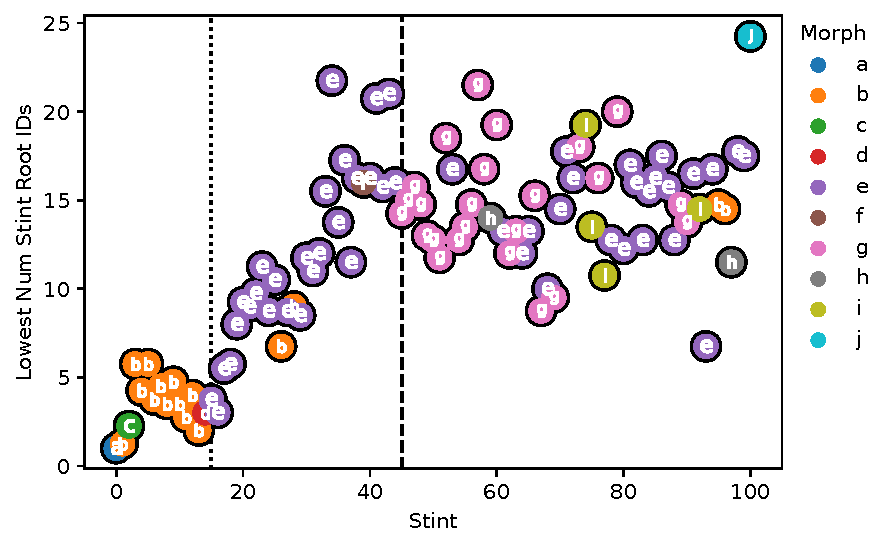
\includegraphics[width=\linewidth]{{plots/phylogeny/bucket=prq49+cat=morph+endeavor=16+transform=filter-Series-16005+viz=letterscatter-vline+x=stint+y=lowest-num-stint-root-ids+ext=}}

\caption{ Number of genomes with the lowest surviving original phylogenetic root ID from the beginning of a stint with extant offspring at the end of that stint.  }
\label{fig:phylogeny:lowestroot_stint_roots}

\end{subfigure}%
\begin{subfigure}{0.5\textwidth}

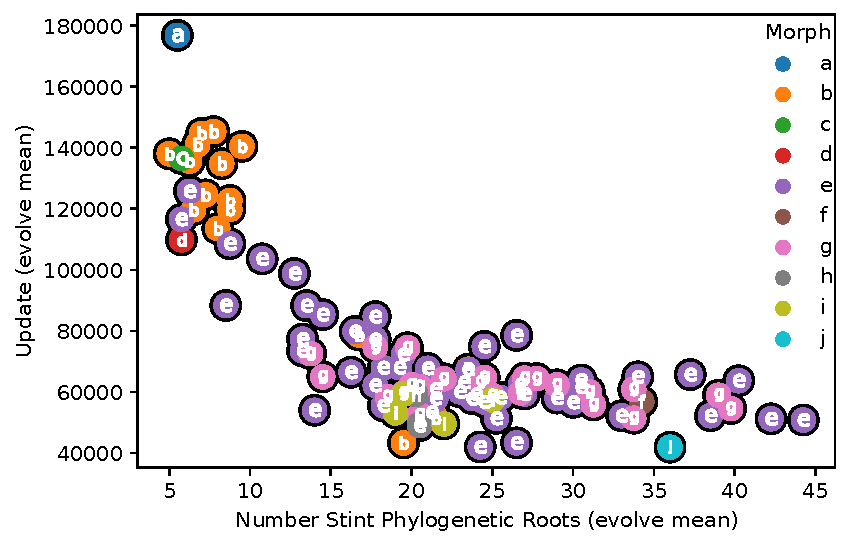
\includegraphics[width=\linewidth]{{plots/simulation/bucket=prq49+cat=morph+endeavor=16+transform=filter-Series-16005+viz=letterscatter+x=number-stint-phylogenetic-roots-evolve-mean+y=update-evolve-mean+ext=}}

\caption{
Relationship between number of simulation updates elapsed in a stint and the number of genomes seeded into a stint with extant descendants at the end of that stint.
}
\label{fig:phylogeny:updates_vs_stint_roots}

\end{subfigure}%

\begin{subfigure}{0.5\textwidth}

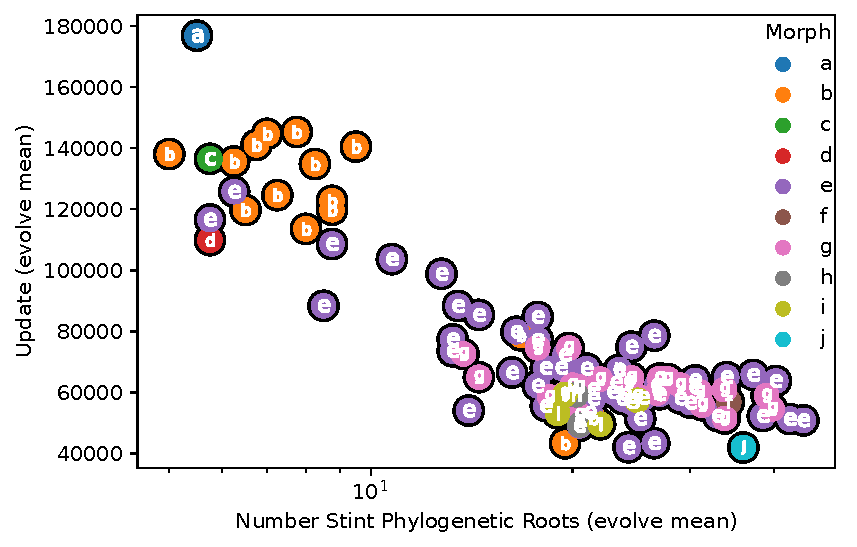
\includegraphics[width=\linewidth]{{plots/simulation/bucket=prq49+cat=morph+endeavor=16+transform=filter-Series-16005+viz=log-letterscatter+x=number-stint-phylogenetic-roots-evolve-mean+y=update-evolve-mean+ext=}}

\caption{ Relationship between number of simulation updates elapsed in a stint and the number of genomes seeded into a stint with extant descendants at the end of that stint, log axis. }
\label{fig:phylogeny:log_updates_vs_stint_roots}

\end{subfigure}%


\caption{
Phylogenetic statistics.
Color coding and letters correspond to qualitative morph codes described in Table \ref{tab:morph_descriptions}.
Dotted vertical line denotes emergence of morph $e$.
Dashed vertical line denotes emergence of morph $g$.
}
\label{fig:phylogeny}
\end{figure*}

\begin{figure*}
\centering
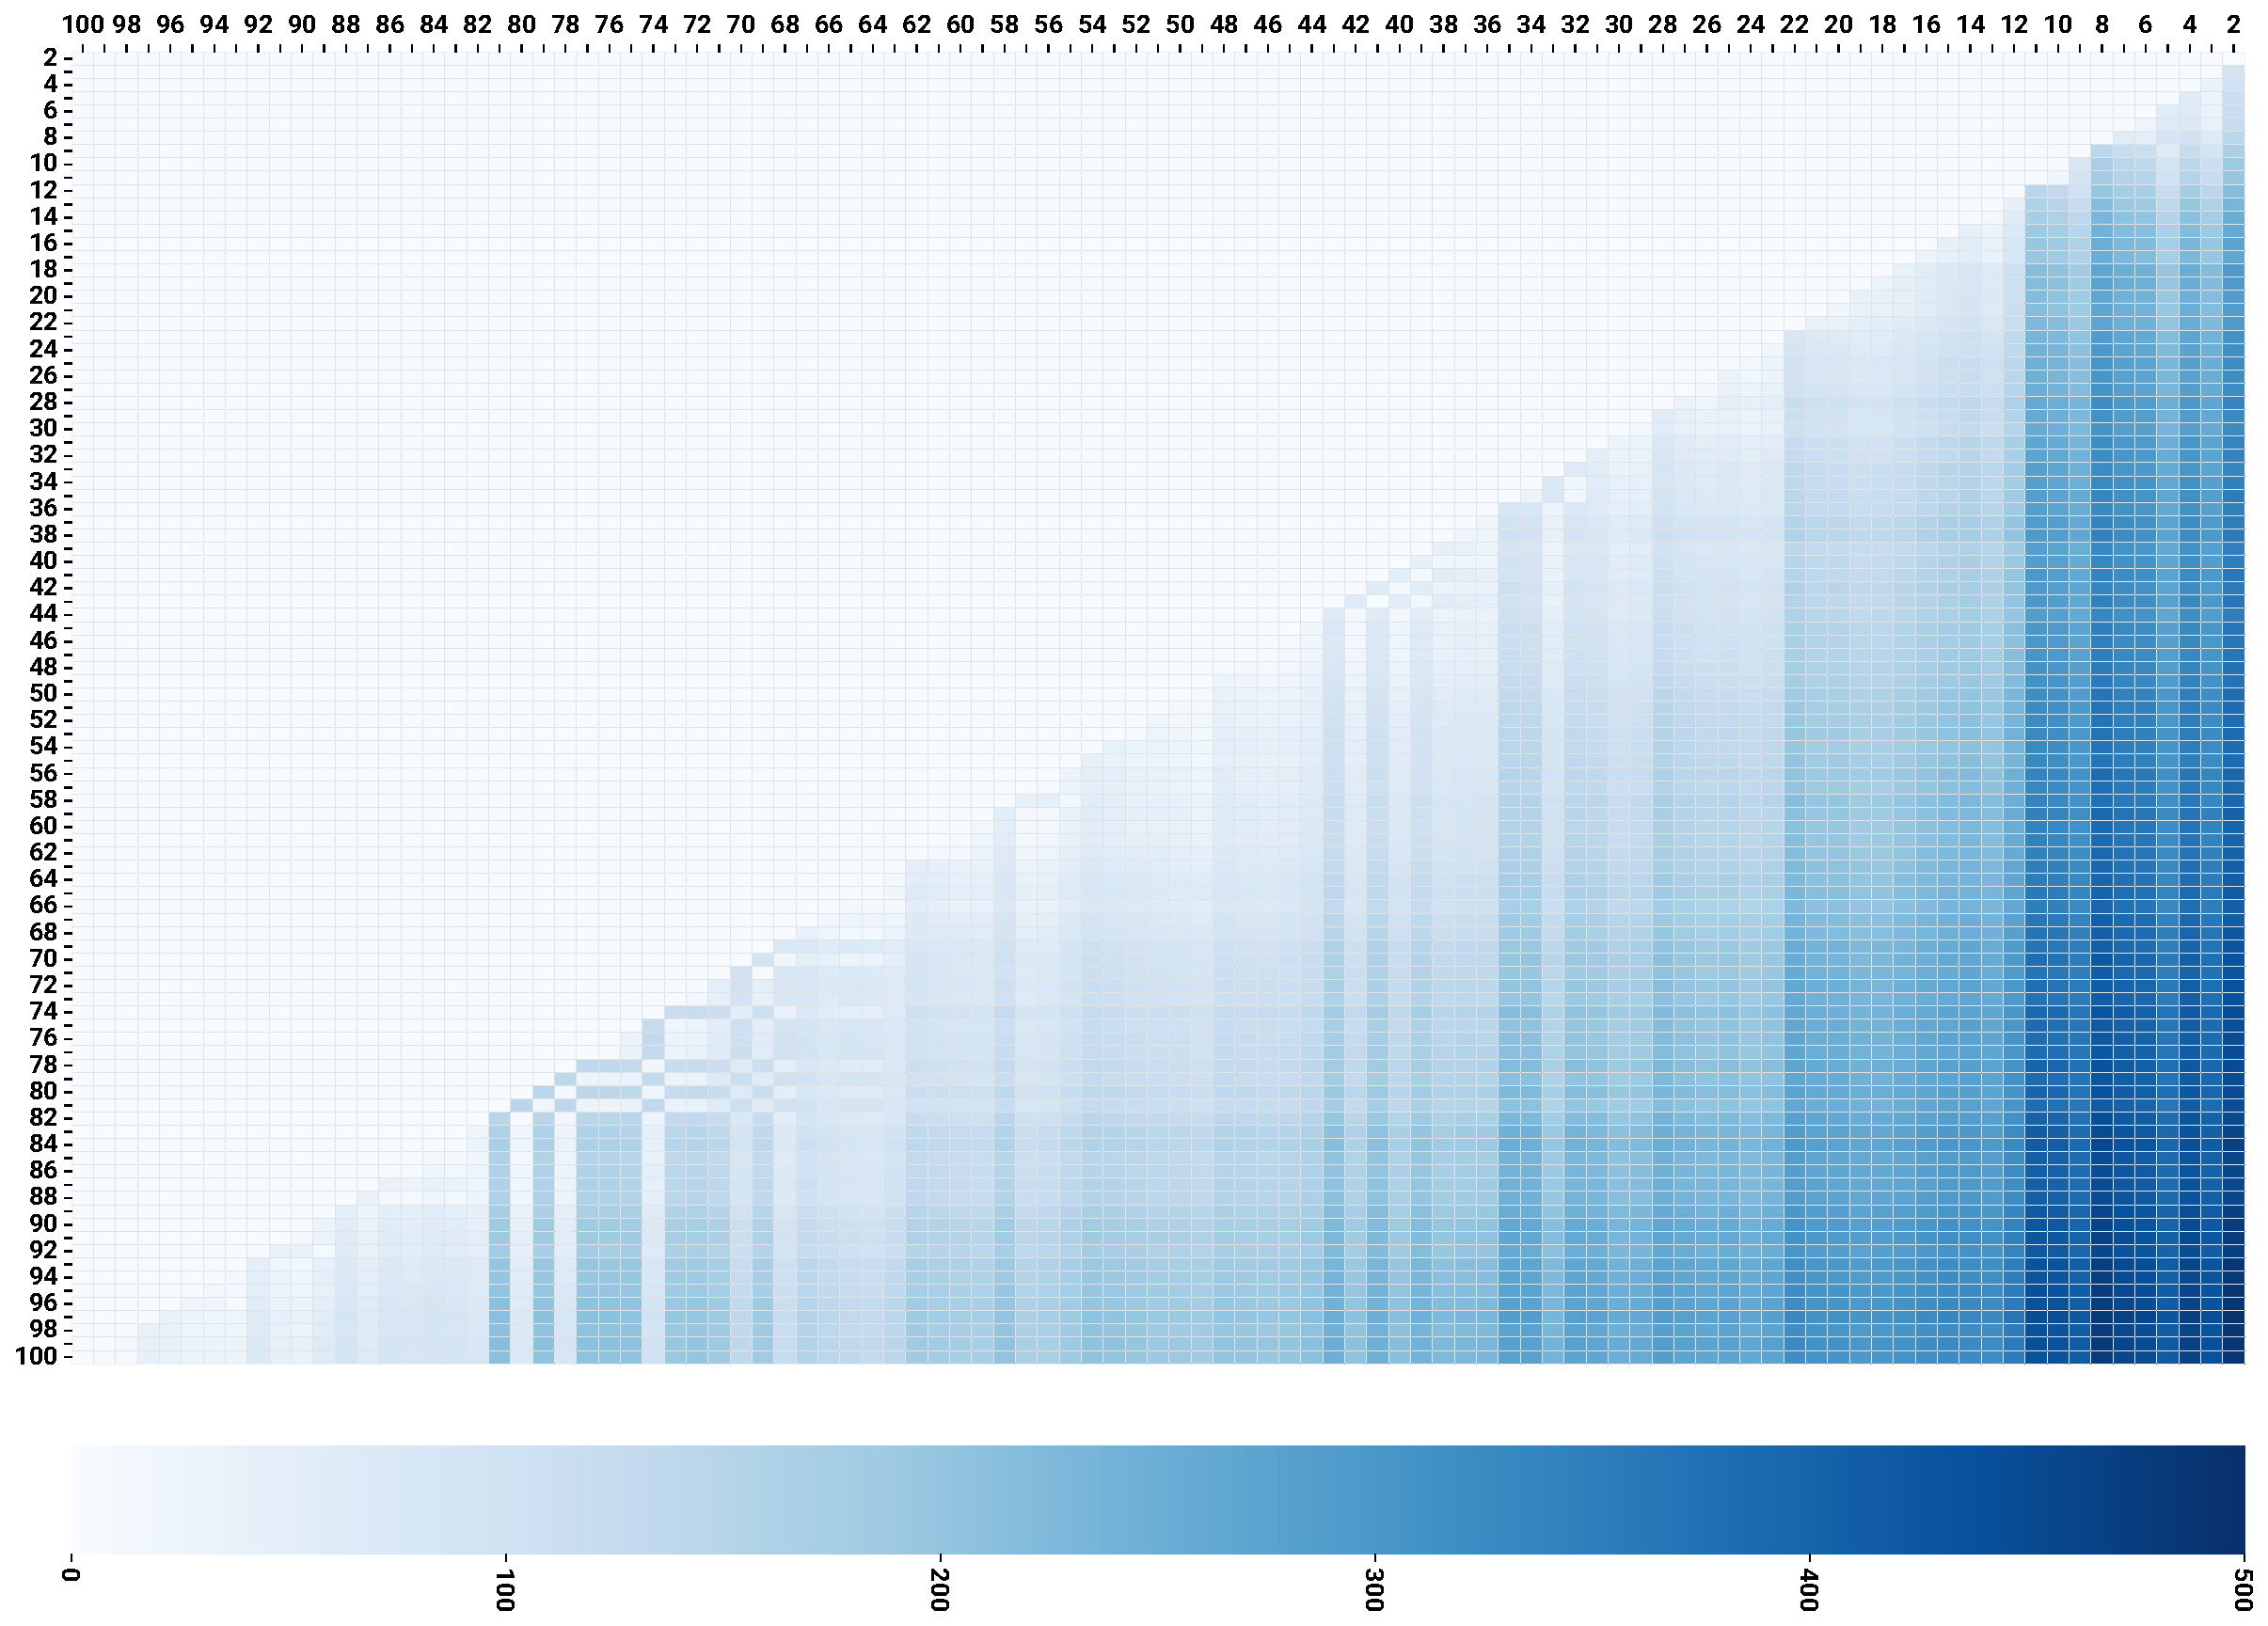
\includegraphics[width=0.8\linewidth]{{submodule/dishtiny_event_tag_phylogenetics/teeplots/distance_matrix_no_outliers/cmap=blues+linecolor=88888820+viz=heatmap+ext=}}

\caption{
TODO
}
\label{fig:phylo_distance_matrix_heatmap}
\end{figure*}



\begin{figure*}

\begin{subfigure}{0.5\textwidth}

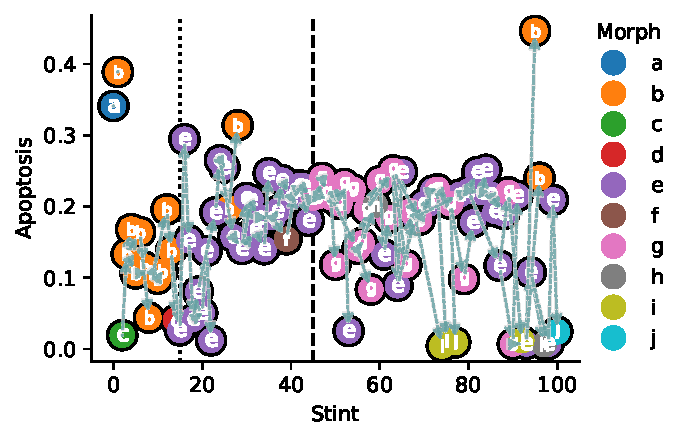
\includegraphics[width=\linewidth]{{plots/apoptosis_stint/bucket=prq49+cat=morph+endeavor=16+transform=filter-Series-16005+viz=letterscatter-vline+x=stint+y=fraction-deaths-apoptosis-monoculture-mean+ext=}}

\caption{Fraction of cell deaths due to apoptosis.
Color coding and letters correspond to qualitative morph codes described in Table \ref{tab:morph_descriptions}.}
\label{fig:apoptosis:apoptosis_stint}

\end{subfigure}%

\begin{subfigure}{0.5\textwidth}

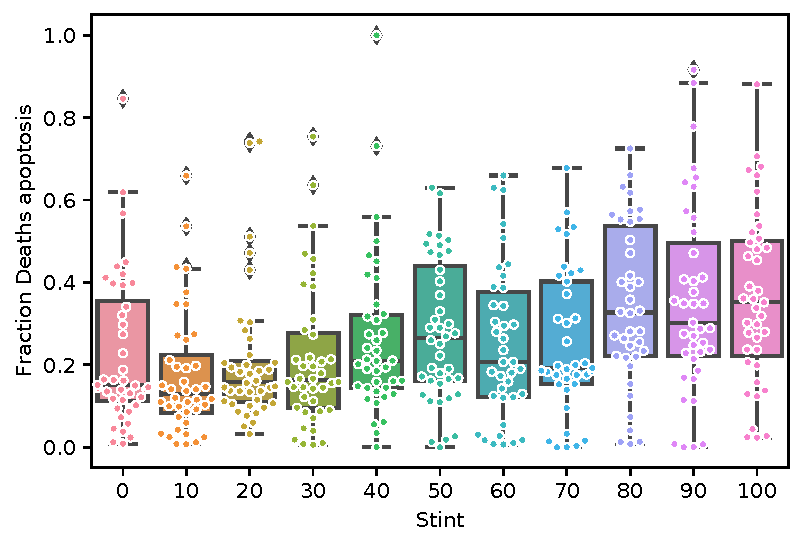
\includegraphics[width=\linewidth]{{plots/apoptosis_distn/bucket=prq49+endeavor=16+transform=filter-Stint-mod10+viz=swarmplot-boxplot+x=stint+y=fraction-deaths-apoptosis+ext=}}

\caption{Distribution of apoptosis rates across evolutionary replicates.}
\label{fig:apoptosis:apoptosis_distn}

\end{subfigure}%


\caption{ Apoptosis rates in case study strain and across evolutionary replicates. }
\label{fig:apoptosis}
\end{figure*}

\begin{figure}

\begin{subfigure}{0.5\textwidth}

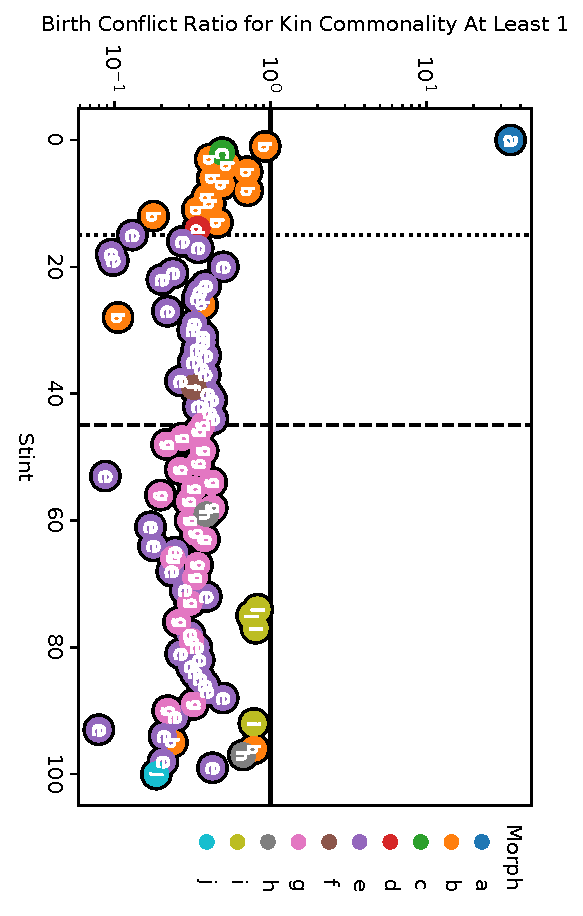
\includegraphics[width=\linewidth]{{plots/conflict/at_least_one/bucket=prq49+cat=morph+endeavor=16+transform=filter-Series-16005+viz=log-letterscatter-vline-hline+x=stint+y=birth-conflict-ratio-for-kin-commonality-at-least-1+ext=}}

\caption{
Frequency at which cell proliferation replaces neighbors with any kin group commonality to the parent, normalized for the relative frequency of neighbors with kin group commonality to the parent.
Values below 1.0 (horizontal bar) indicate preference to displace neighbors with no kin group commonality.
}
\label{fig:conflict:at_least_one}

\end{subfigure}%
\begin{subfigure}{0.5\textwidth}

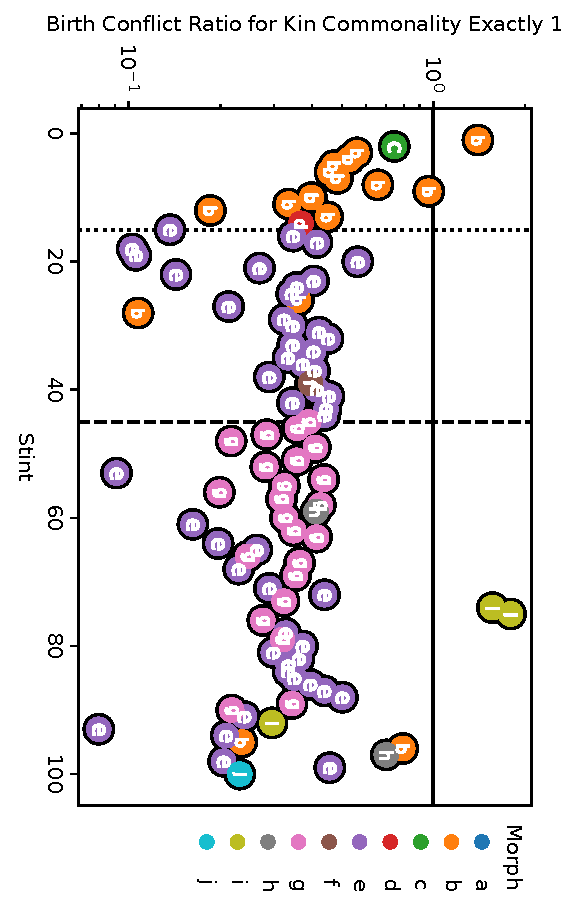
\includegraphics[width=\linewidth]{{plots/conflict/exactly_one/bucket=prq49+cat=morph+endeavor=16+transform=filter-Series-16005+viz=log-letterscatter-vline-hline+x=stint+y=birth-conflict-ratio-for-kin-commonality-exactly-1+ext=}}

\caption{
Frequency at which cell proliferation replaces neighbors with only outer kin group commonality to the parent, normalized for the relative frequency of neighbors with kin group commonality to the parent.
Values below 1.0 (horizontal bar) indicate preference to displace neighbors with no kin group commonality.
}
\label{fig:conflict:exactly_one}

\end{subfigure}%

\begin{subfigure}{0.5\textwidth}

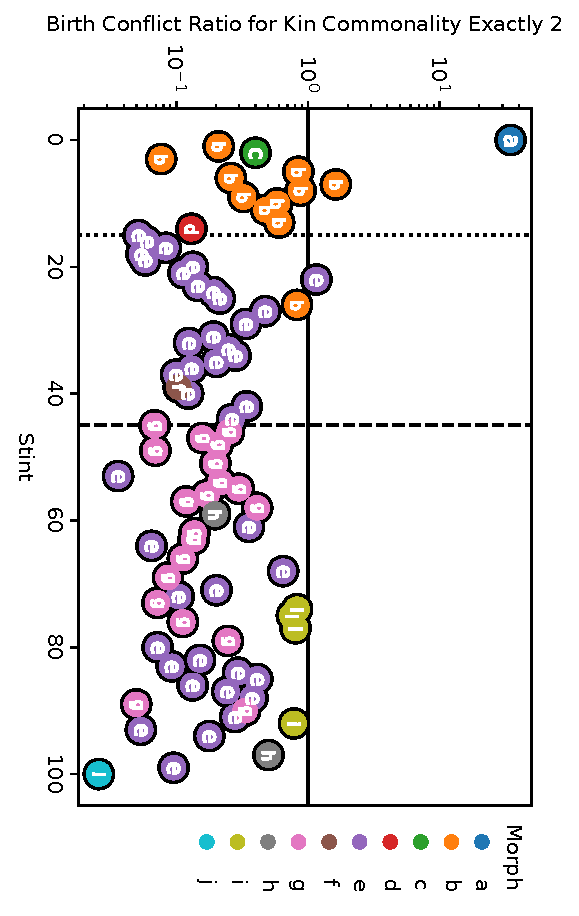
\includegraphics[width=\linewidth]{{plots/conflict/exactly_two/bucket=prq49+cat=morph+endeavor=16+transform=filter-Series-16005+viz=log-letterscatter-vline-hline+x=stint+y=birth-conflict-ratio-for-kin-commonality-exactly-2+ext=}}

\caption{
Frequency at which cell proliferation replaces neighbors with full kin group commonality to the parent, normalized for the relative frequency of neighbors with kin group commonality to the parent.
Values below 1.0 (horizontal bar) indicate preference to displace neighbors without full kin group commonality.
}
\label{fig:conflict:exactly_two}

\end{subfigure}%


\caption{ Kin conflict rates.
Color coding and letters correspond to qualitative morph codes described in Table \ref{tab:morph_descriptions}.}
\label{fig:conflict}

\end{figure}
\begin{figure*}

\begin{subfigure}{0.5\textwidth}

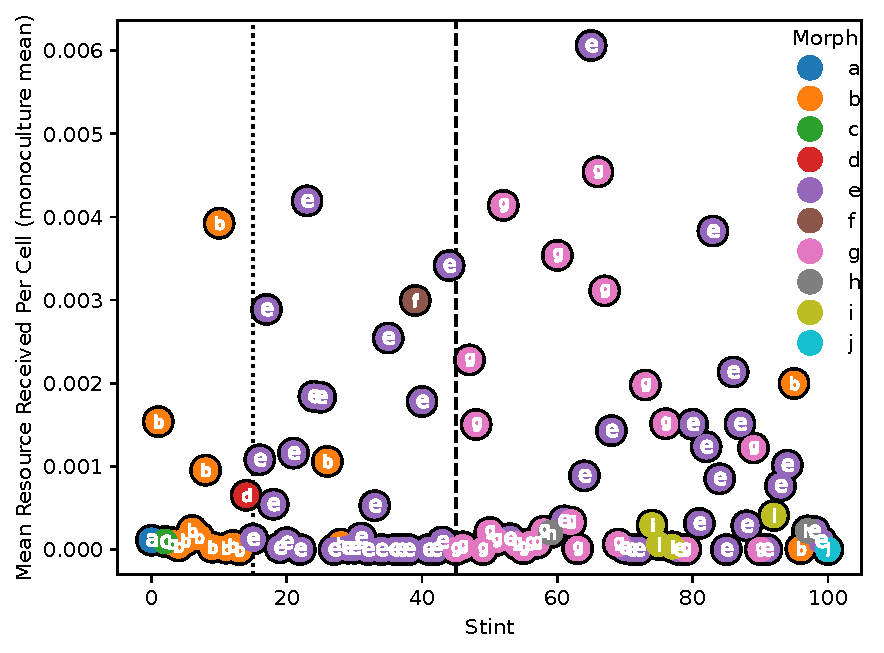
\includegraphics[width=\linewidth]{{plots/resource_sharing/bucket=prq49+cat=morph+endeavor=16+transform=filter-Series-16005+viz=letterscatter-vline+x=stint+y=mean-resource-received-per-cell-monoculture-mean+ext=}}

\caption{ Fraction of cells receiving shared resource at end of evolutionary stints, including not just the focal lineage. }
\label{fig:resource_sharing:fraction_sharing_evolve}

\end{subfigure}%

\begin{subfigure}{0.5\textwidth}

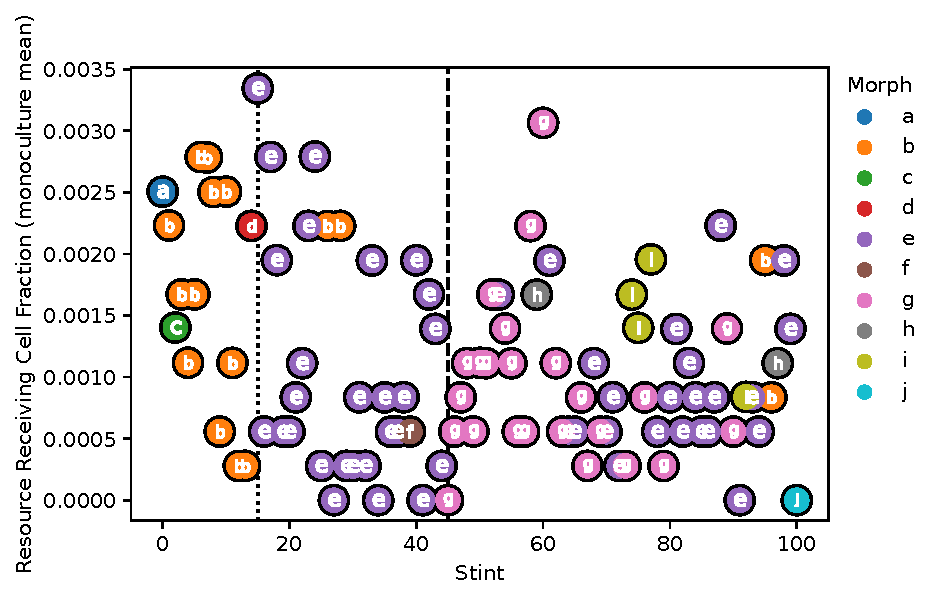
\includegraphics[width=\linewidth]{{plots/resource_sharing/bucket=prq49+cat=morph+endeavor=16+transform=filter-Series-16005+viz=letterscatter-vline+x=stint+y=resource-receiving-cell-fraction-monoculture-mean+ext=}}

\caption{ Fraction of cells receiving shared resource in monocultures of focal lineage. }
\label{fig:resource_sharing:fraction_sharing_monoculture}

\end{subfigure}%

\begin{subfigure}{0.5\textwidth}

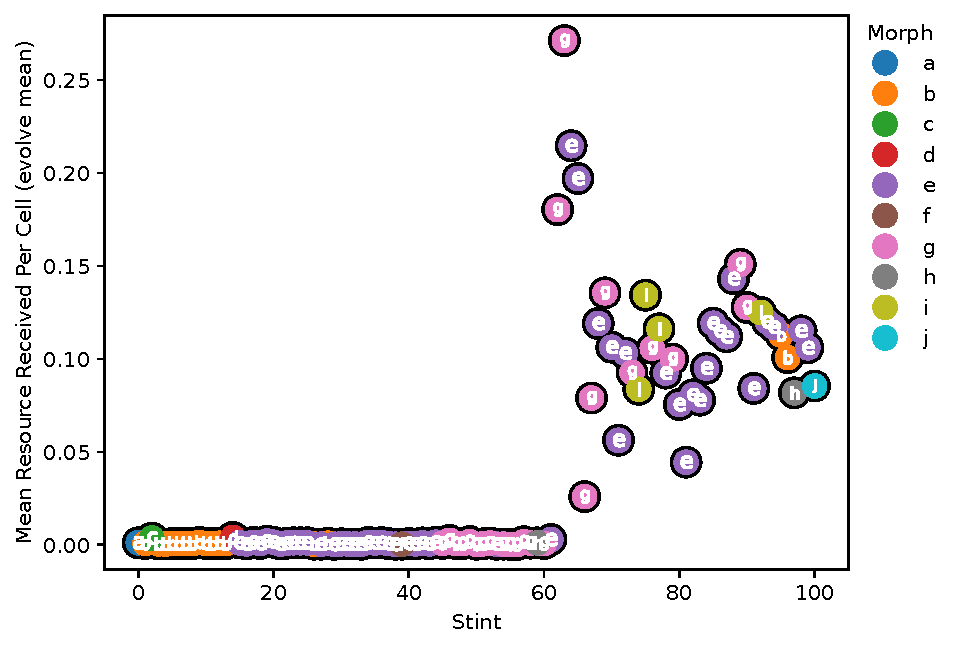
\includegraphics[width=\linewidth]{{plots/resource_sharing/bucket=prq49+cat=morph+endeavor=16+transform=filter-Series-16005+viz=letterscatter+x=stint+y=mean-resource-received-per-cell-evolve-mean+ext=}}

\caption{ Mean amount of resource shared per cell-update at end of evolutionary stints, including not just the focal lineage. }
\label{fig:resource_sharing:sharing_amount_evolve}

\end{subfigure}%
\begin{subfigure}{0.5\textwidth}

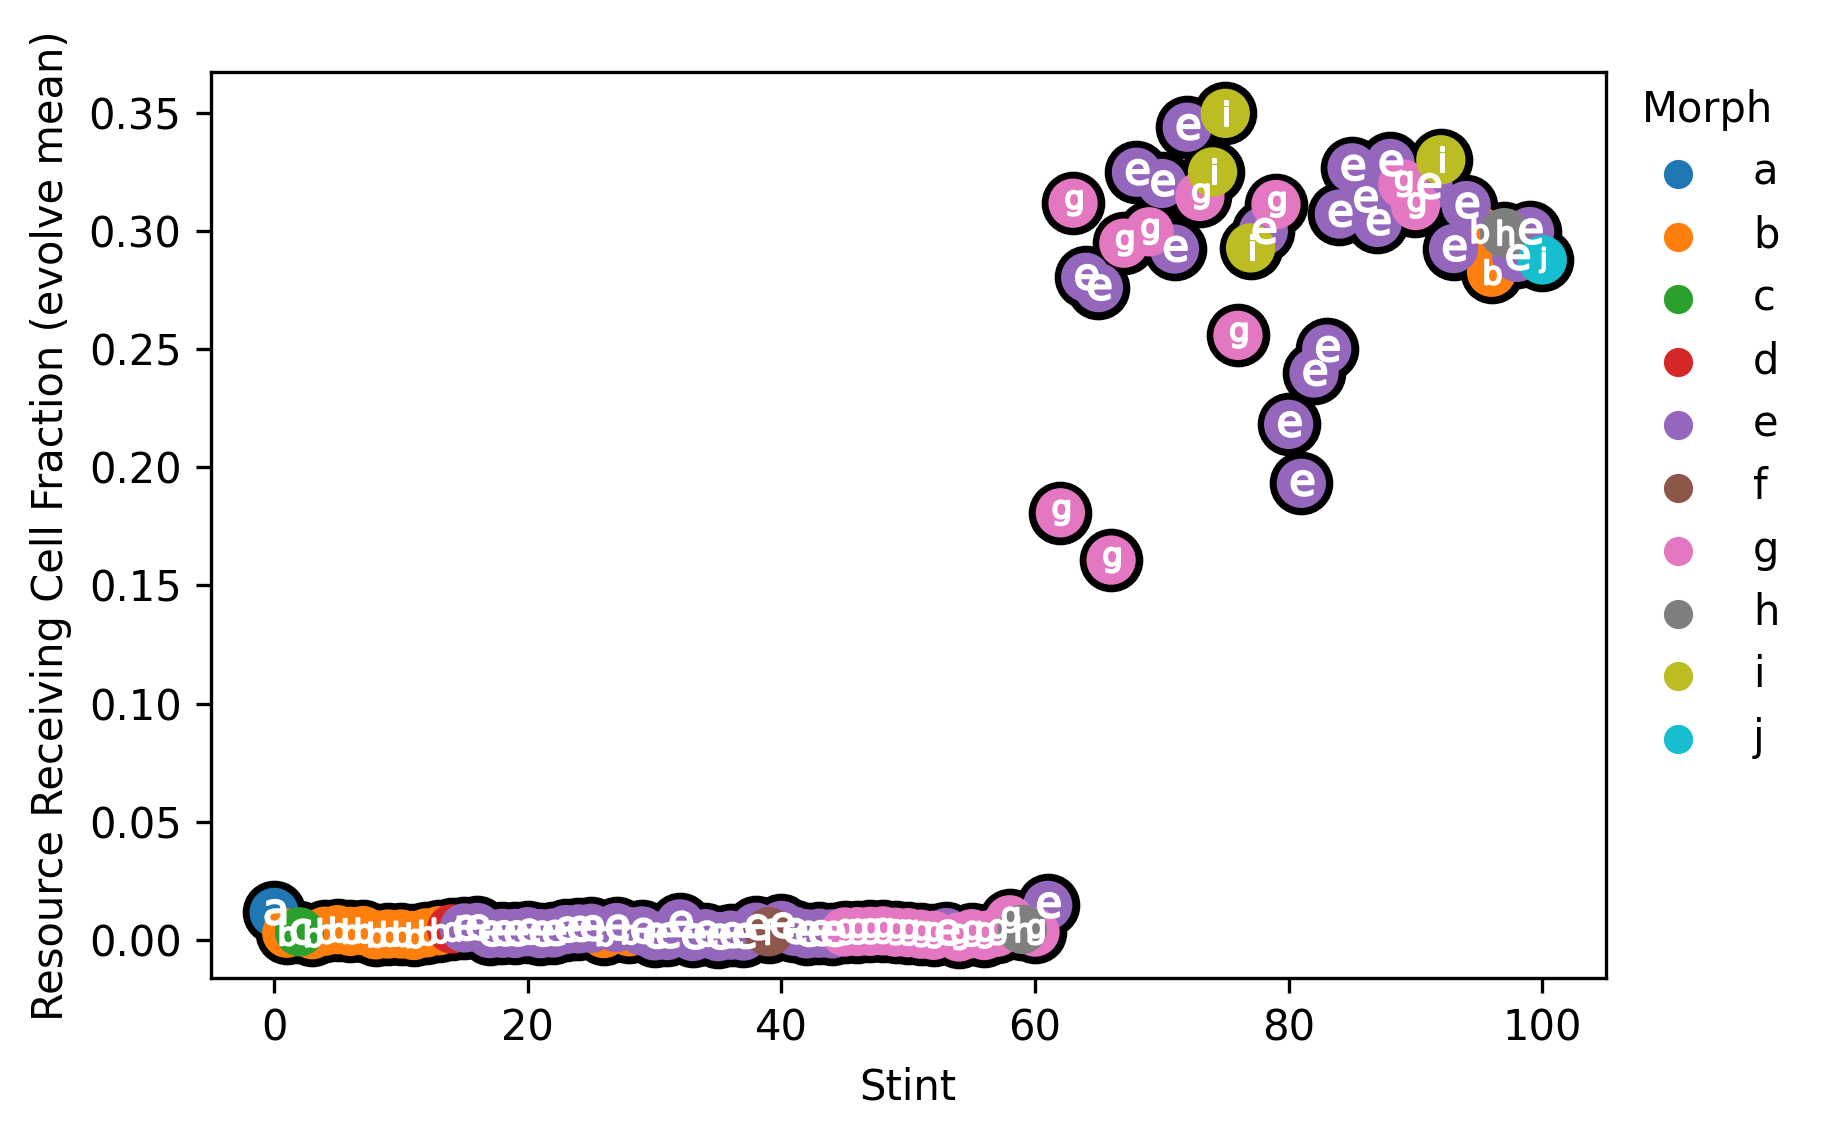
\includegraphics[width=\linewidth]{{plots/resource_sharing/bucket=prq49+cat=morph+endeavor=16+transform=filter-Series-16005+viz=letterscatter+x=stint+y=resource-receiving-cell-fraction-evolve-mean+ext=}}

\caption{Mean amount of resource shared per cell-update in monocultures of focal lineage. }
\label{fig:resource_sharing:sharing_amount_monoculture}

\end{subfigure}%


\caption{
\textbf{Resource-sharing phenotypic traits.}
\footnotesize
Color coding and letters correspond to qualitative morph codes described in Table \ref{tab:morph_descriptions}.
Dotted vertical line denotes emergence of morph $e$.
Dashed vertical line denotes emergence of morph $g$.
}
\label{fig:resource_sharing}
\end{figure*}

\begin{figure*}

\begin{subfigure}{0.5\textwidth}

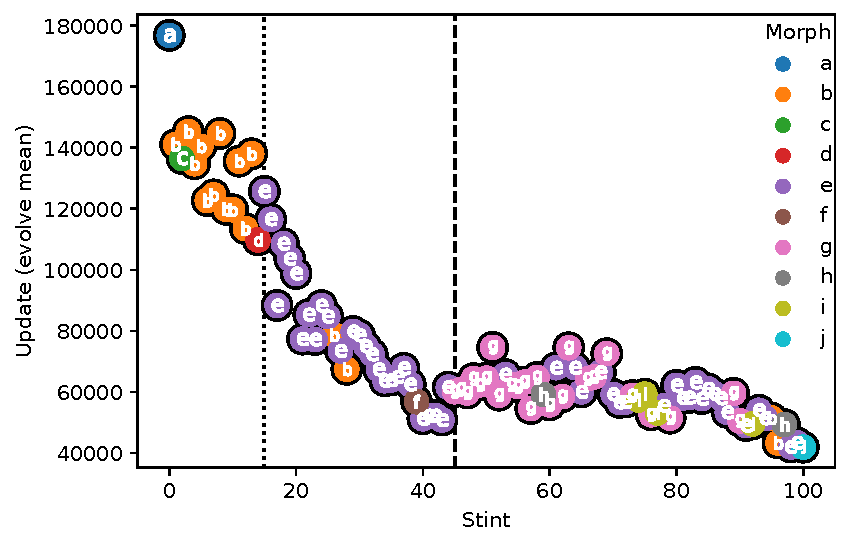
\includegraphics[width=\linewidth]{{plots/simulation/bucket=prq49+cat=morph+endeavor=16+transform=filter-Series-16005+viz=letterscatter-vline+x=stint+y=update-evolve-mean+ext=}}

\caption{ Number simulation updates elapsed per three-hour evolutionary stint. Color coding and letters correspond to qualitative morph codes described in Table \ref{tab:morph_descriptions}. }
\label{fig:simulation:stint_updates}

\end{subfigure}%

\begin{subfigure}{0.5\textwidth}

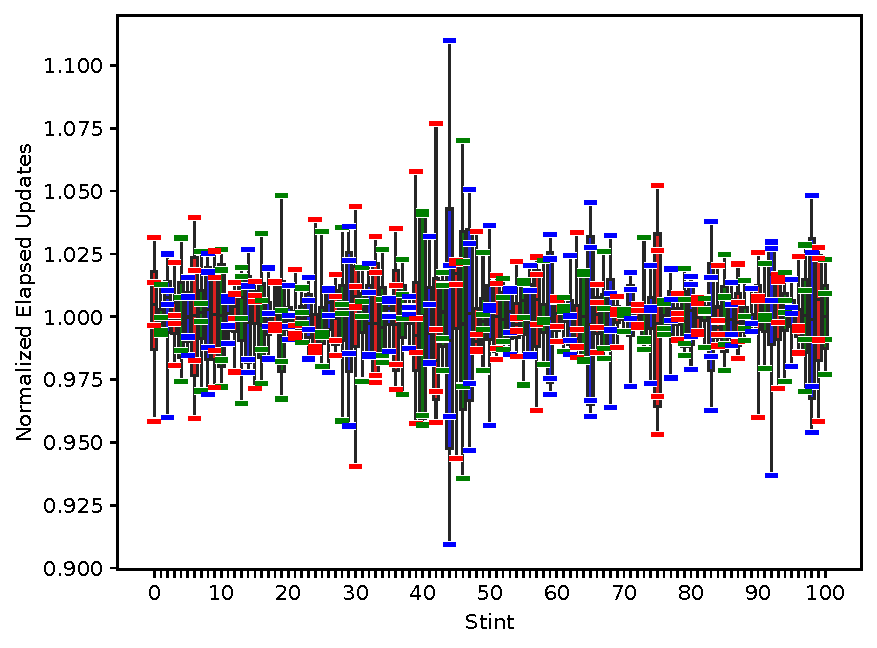
\includegraphics[width=\linewidth]{{plots/simulation/bucket=prq49+endeavor=16+hue=stint+transform=filter-Series-16005+viz=boxstrip+x=stint+y=normalized-elapsed-updates+ext=}}

\caption{ Distribution of real-time simulation rate of concurrent threads. Colors provided only to distinguish neighboring data. }
\label{fig:simulation:thread_updates}

\end{subfigure}%

\caption{ Real-time simulation performance. }
\label{fig:simulation}
\end{figure*}



\begin{sidewaysfigure*}
\centering
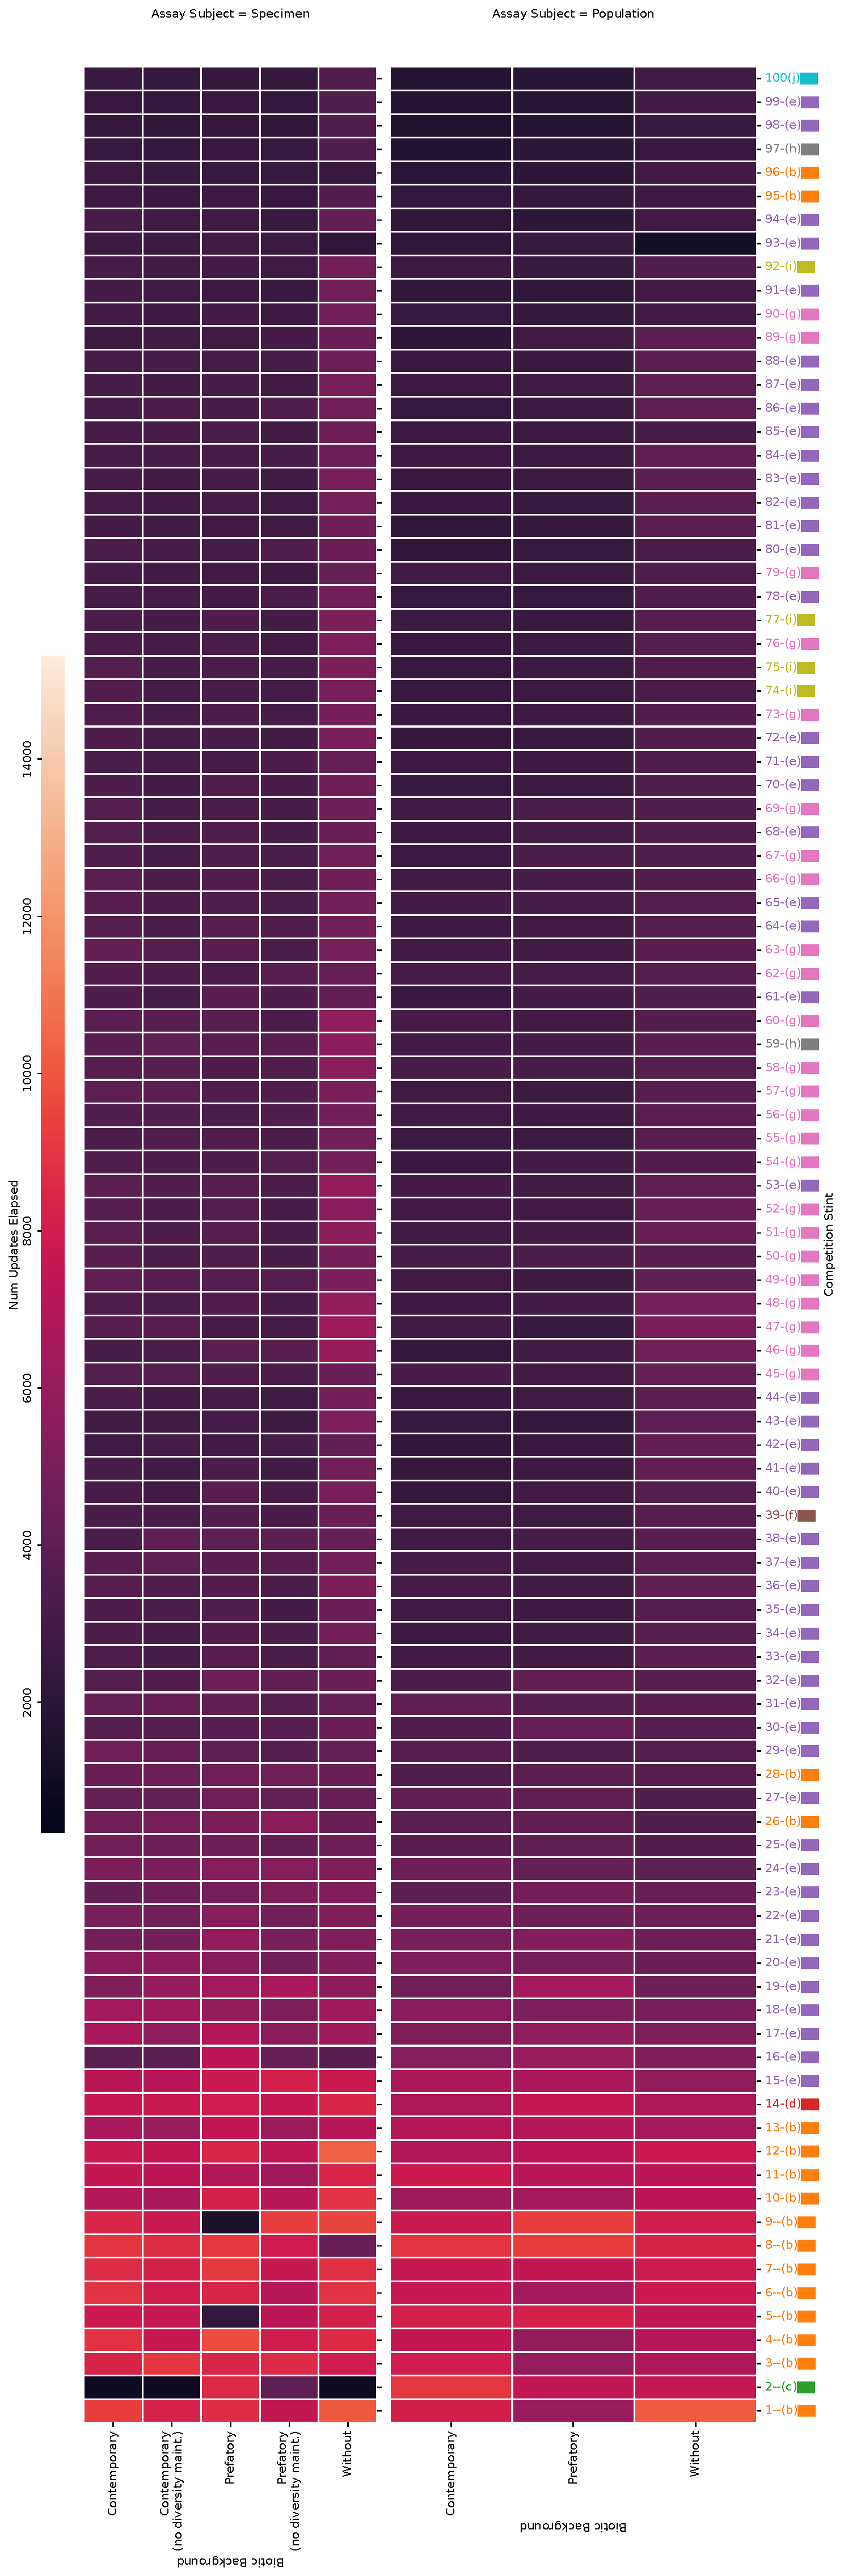
\includegraphics[width=\linewidth]{{submodule/dishtiny/binder/bucket=prq49/a=adaptation_assays+endeavor=16/teeplots/hue=num-updates-elapsed+viz=facet-heatmap+x=biotic-background+y=competition-stint+ext=}}

\caption{
Number updates elapsed during fixed-duration adaptation assay competitions for sampled representative specimen (top) population-level adaptation (bottom).
See Figure \ref{fig:adaptation_assay_cartoon} for explanation of competition biotic backgrounds.
See Supplementary Figure \ref{fig:num_updates_elapsed_barplot} for confidence interval estimates of mean updates elapsed during competition expedriments and Supplementary Figure \ref{fig:num_updates_elapsed_boxplot} for distributions of updates elapsed during competition experiments.
}
\label{fig:num_updates_elapsed_heatmap}
\end{sidewaysfigure*}


\begin{sidewaysfigure*}
\thisfloatpagestyle{mylandscape}%
\rotatesidewayslabel%
\centering
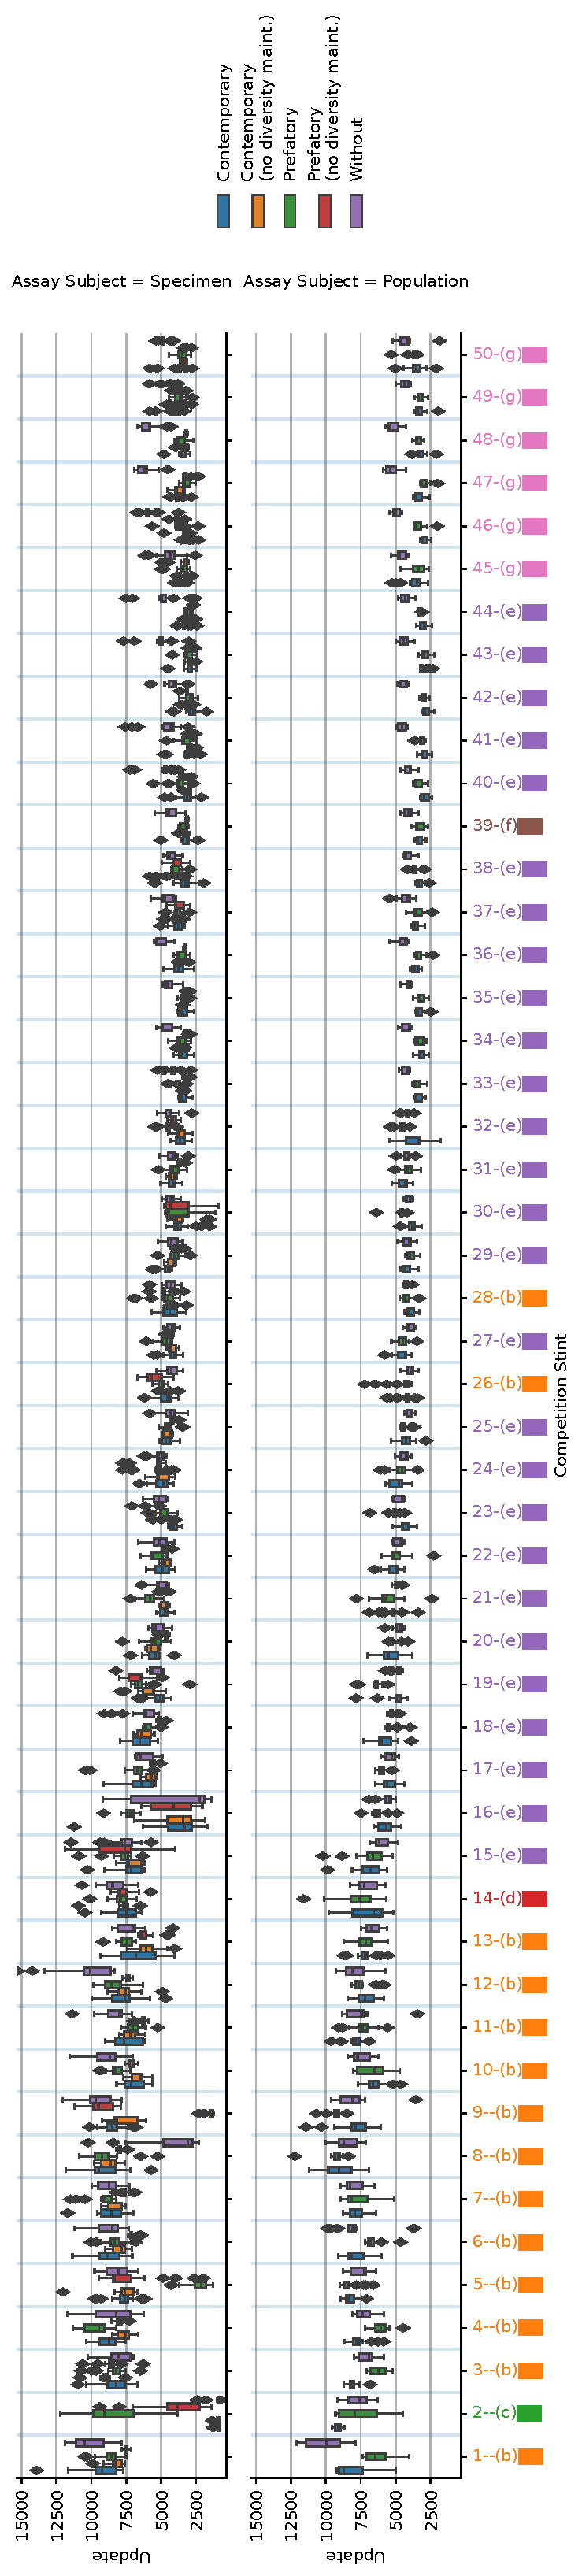
\includegraphics[width=\linewidth]{{submodule/dishtiny/binder/bucket=prq49/a=adaptation_assays+endeavor=16/teeplots/hue=biotic-background+stint=1-50+viz=facet-boxplot+x=competition-stint+y=update+ext=}}
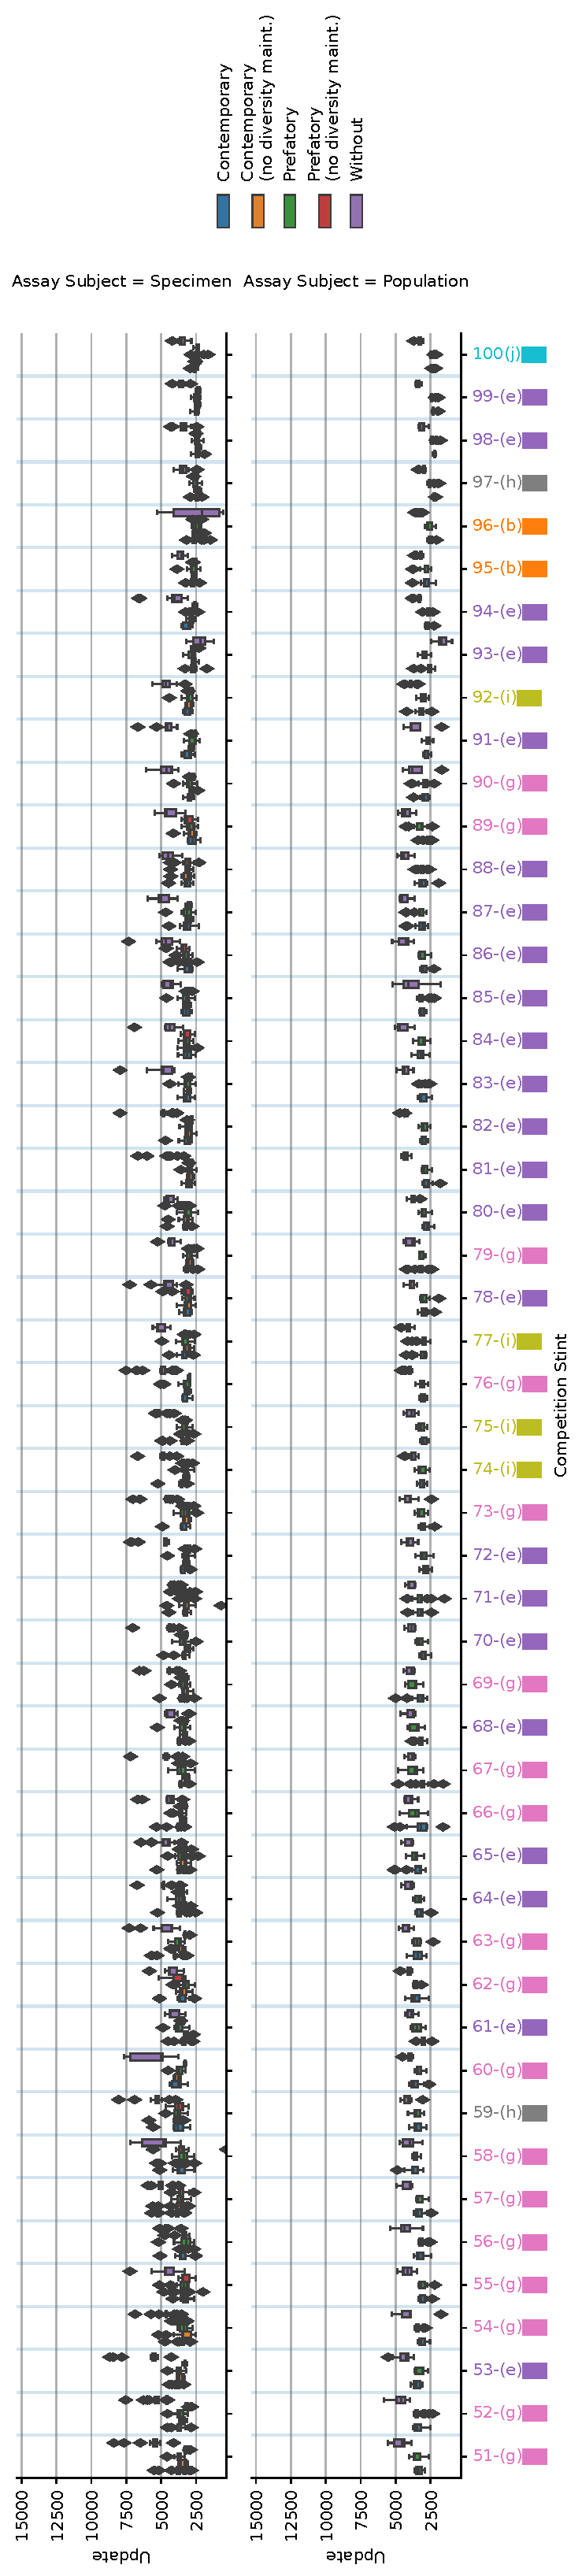
\includegraphics[width=\linewidth]{{submodule/dishtiny/binder/bucket=prq49/a=adaptation_assays+endeavor=16/teeplots/hue=biotic-background+stint=51-100+viz=facet-boxplot+x=competition-stint+y=update+ext=}}

\caption{
\textbf{Number updates elapsed during fixed-duration adaptation assay competitions.}
\footnotesize
For sampled representative specimen (upper panels) and population-level adaptation (lower panels).
Figure is split into two rows due to layout considerations.
See Figure \ref{fig:adaptation_assay_cartoon} for explanation of competition biotic backgrounds.
}
\label{fig:num_updates_elapsed_boxplot}
\end{sidewaysfigure*}


\begin{sidewaysfigure*}
\thisfloatpagestyle{mylandscape}%
\rotatesidewayslabel%
\centering
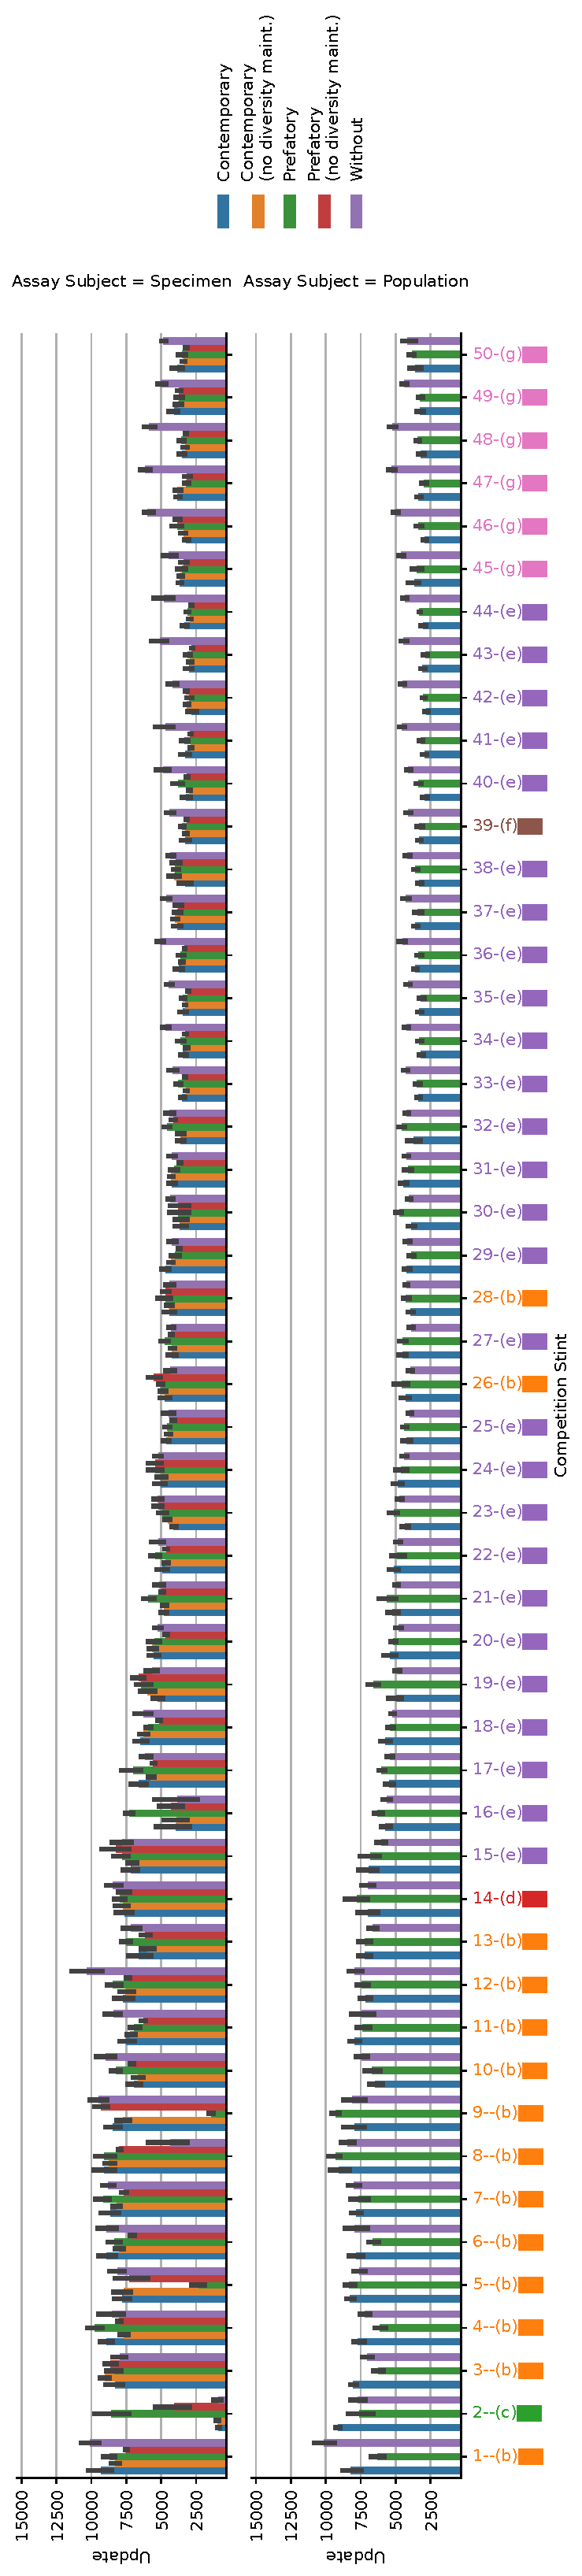
\includegraphics[width=\linewidth]{{submodule/dishtiny/binder/bucket=prq49/a=adaptation_assays+endeavor=16/teeplots/hue=biotic-background+stint=1-50+viz=facet-barplot+x=competition-stint+y=update+ext=}}
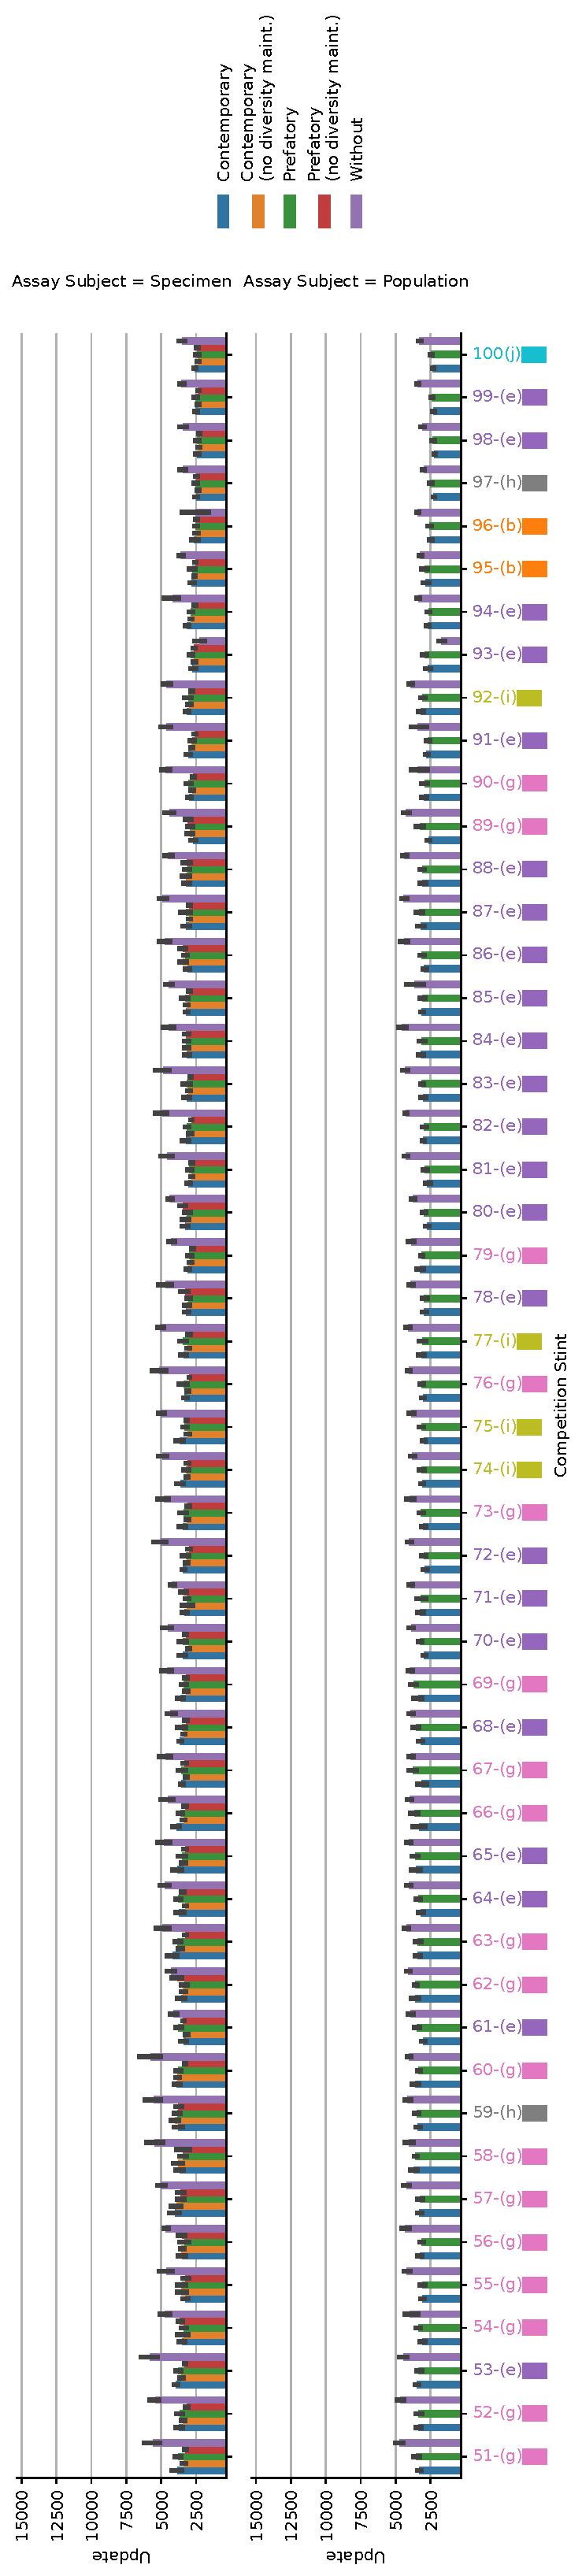
\includegraphics[width=\linewidth]{{submodule/dishtiny/binder/bucket=prq49/a=adaptation_assays+endeavor=16/teeplots/hue=biotic-background+stint=51-100+viz=facet-barplot+x=competition-stint+y=update+ext=}}

\caption{
Number updates elapsed during fixed-duration adaptation assay competitions for sampled representative specimen (upper panels) population-level adaptation (lower panels).
Error bars are bootstrapped 95\% confidence intervals.
Figure is split into two rows due to layout considerations.
See Figure \ref{fig:adaptation_assay_cartoon} for explanation of competition biotic backgrounds.
}
\label{fig:num_updates_elapsed_barplot}
\end{sidewaysfigure*}


\begin{sidewaysfigure*}
\thisfloatpagestyle{mylandscape}%
\rotatesidewayslabel%
\centering
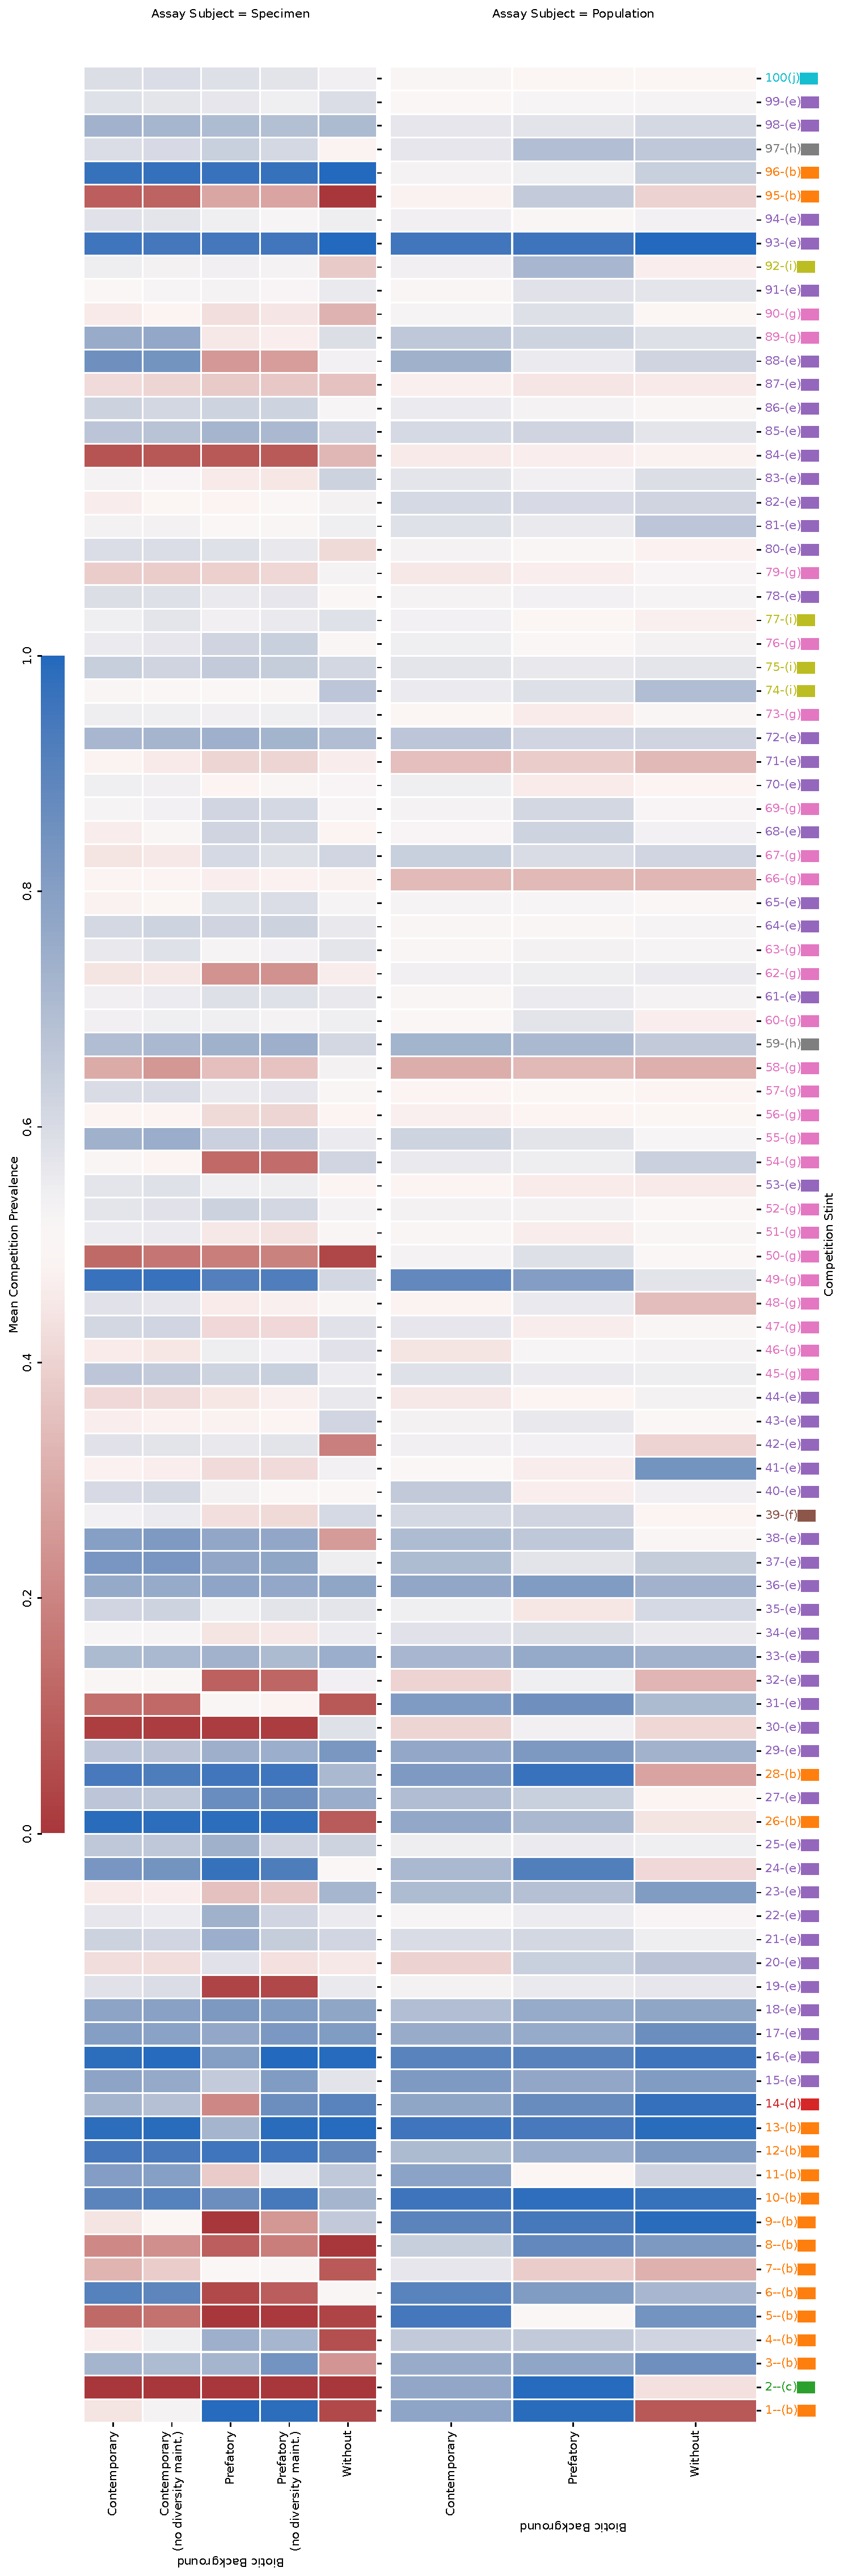
\includegraphics[width=\linewidth]{{submodule/dishtiny/binder/bucket=prq49/a=adaptation_assays+endeavor=16/teeplots/hue=mean-competition-prevalence+viz=facet-heatmap+x=biotic-background+y=competition-stint+ext=}}

\caption{
Mean end-state population composition of competition experiments.
Half (0.5) population composition corresponds to a neutral result, color mapped to white.
Blue indicates fitness gain compared to the previous stint and red indicates fitness loss.
Color coding and parentheticals of stint labels correspond to qualitative morph codes described in Table \ref{tab:morph_descriptions}.
Upper panel shows results for sampled focal strain genome, lower panel shows results for entire focal strain population.
See Figure \ref{fig:adaptation_assay_cartoon} for explanation of competition biotic backgrounds.
See Figure \ref{fig:mean_competition_prevalence_boxplot} for boxplot depiction of prevalence outcomes and Figure \ref{fig:mean_competition_prevalence_barplot} for bootstrapped confidence intervals on mean prevalence outcomes.
}
\label{fig:mean_competition_prevalence}
\end{sidewaysfigure*}


\begin{sidewaysfigure*}
\thisfloatpagestyle{mylandscape}%
\rotatesidewayslabel%
\centering
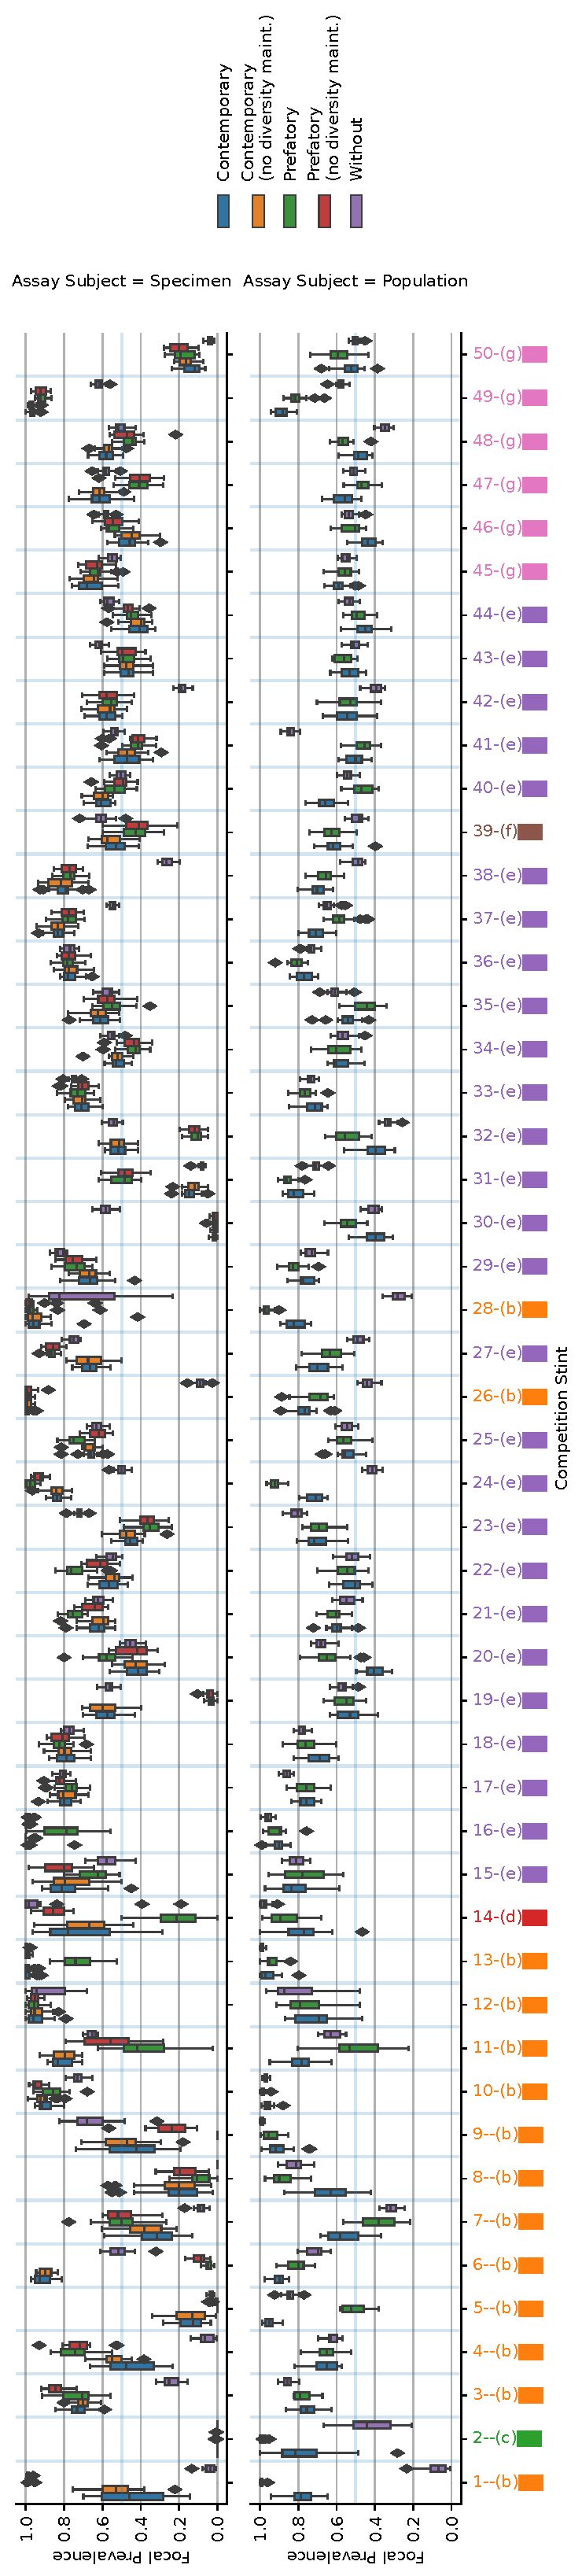
\includegraphics[width=\linewidth]{{submodule/dishtiny/binder/bucket=prq49/a=adaptation_assays+endeavor=16/teeplots/hue=biotic-background+stint=1-50+viz=facet-boxplot+x=competition-stint+y=focal-prevalence+ext=}}

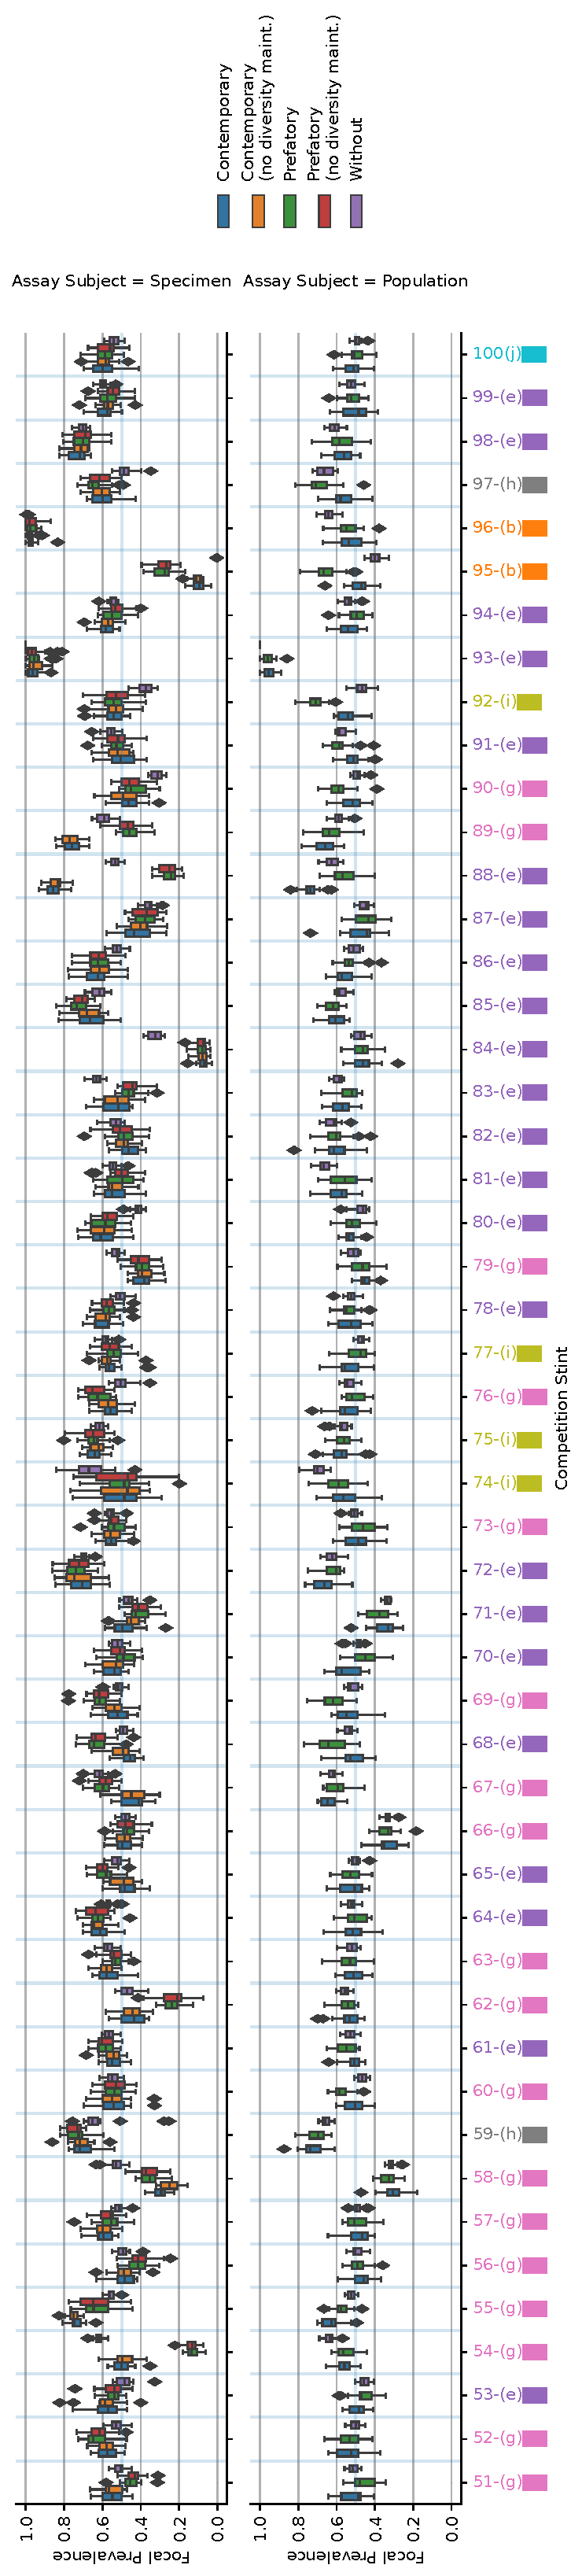
\includegraphics[width=\linewidth]{{submodule/dishtiny/binder/bucket=prq49/a=adaptation_assays+endeavor=16/teeplots/hue=biotic-background+stint=51-100+viz=facet-boxplot+x=competition-stint+y=focal-prevalence+ext=}}

\caption{
\textbf{End-state population composition of competition experiments.}
\footnotesize
Half (0.5) population composition corresponds to a neutral result.
Zero population composition corresponds to extreme fitness loss compared to the previous stint.
Population composition of 1.0 corresponds to extreme fitness gain compared to the previous stint.
Color coding and parentheticals of stint labels correspond to qualitative morph codes described in Table \ref{tab:morph_descriptions}.
Upper panels show results for sampled focal strain genome, lower panels show results for entire focal strain population.
Figure is split into two rows due to layout considerations.
See Figure \ref{fig:adaptation_assay_cartoon} for explanation of competition biotic backgrounds.
See Figure \ref{fig:mean_competition_prevalence_barplot} for bootstrapped confidence intervals on mean prevalence outcomes.
}
\label{fig:mean_competition_prevalence_boxplot}
\end{sidewaysfigure*}


\begin{sidewaysfigure*}
\centering

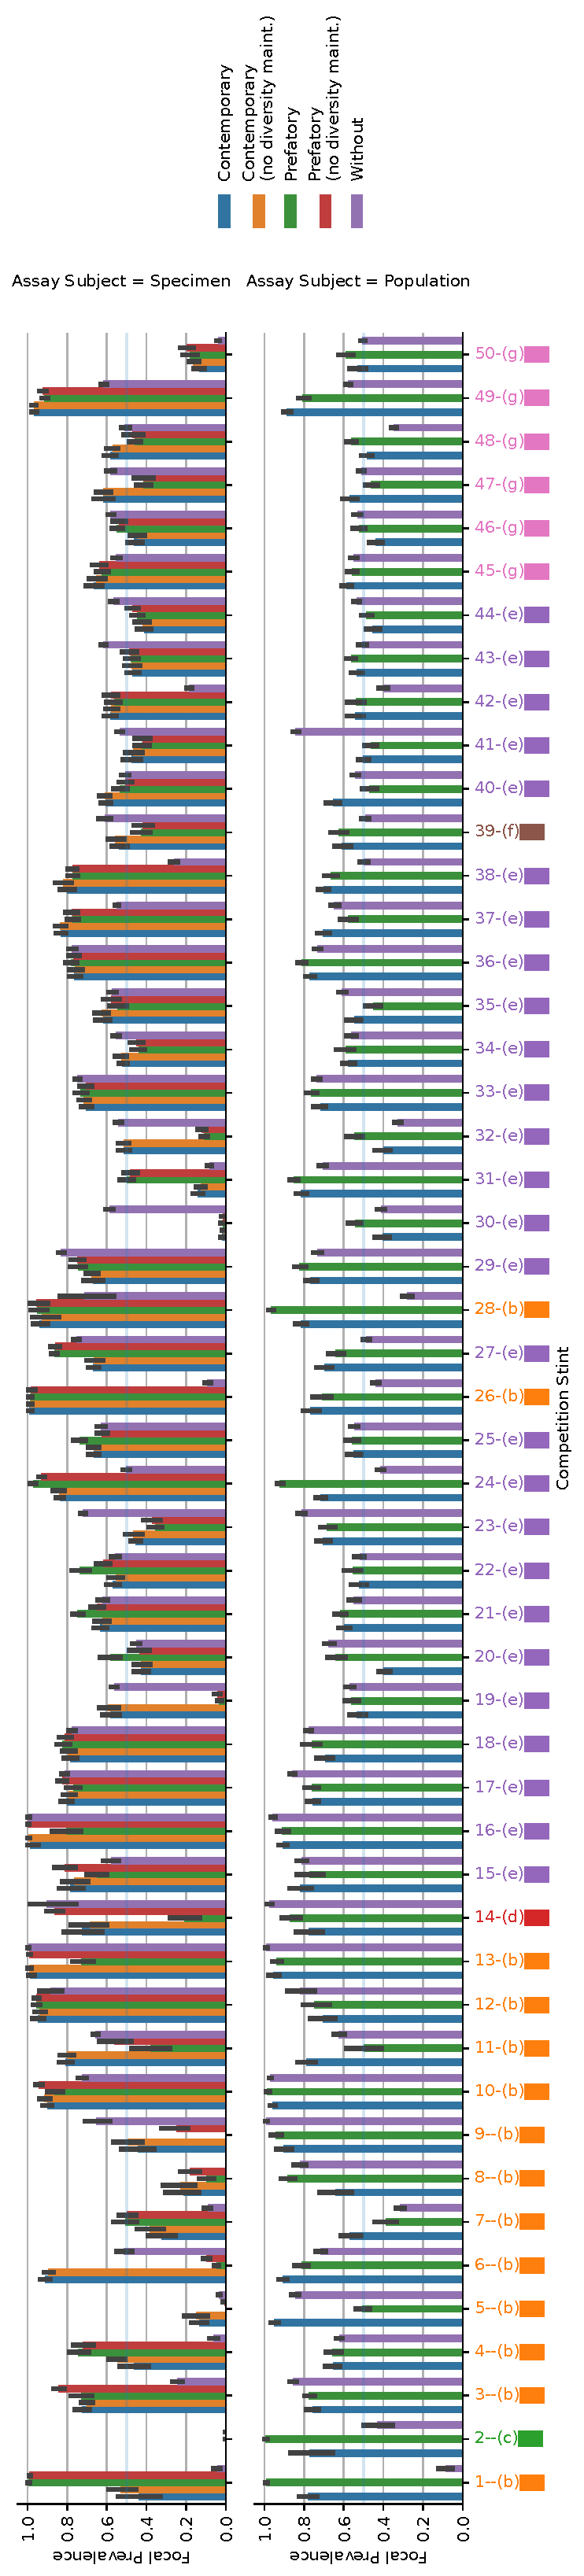
\includegraphics[width=\linewidth]{{submodule/dishtiny/binder/bucket=prq49/a=adaptation_assays+endeavor=16/teeplots/hue=biotic-background+stint=1-50+viz=facet-barplot+x=competition-stint+y=focal-prevalence+ext=}}

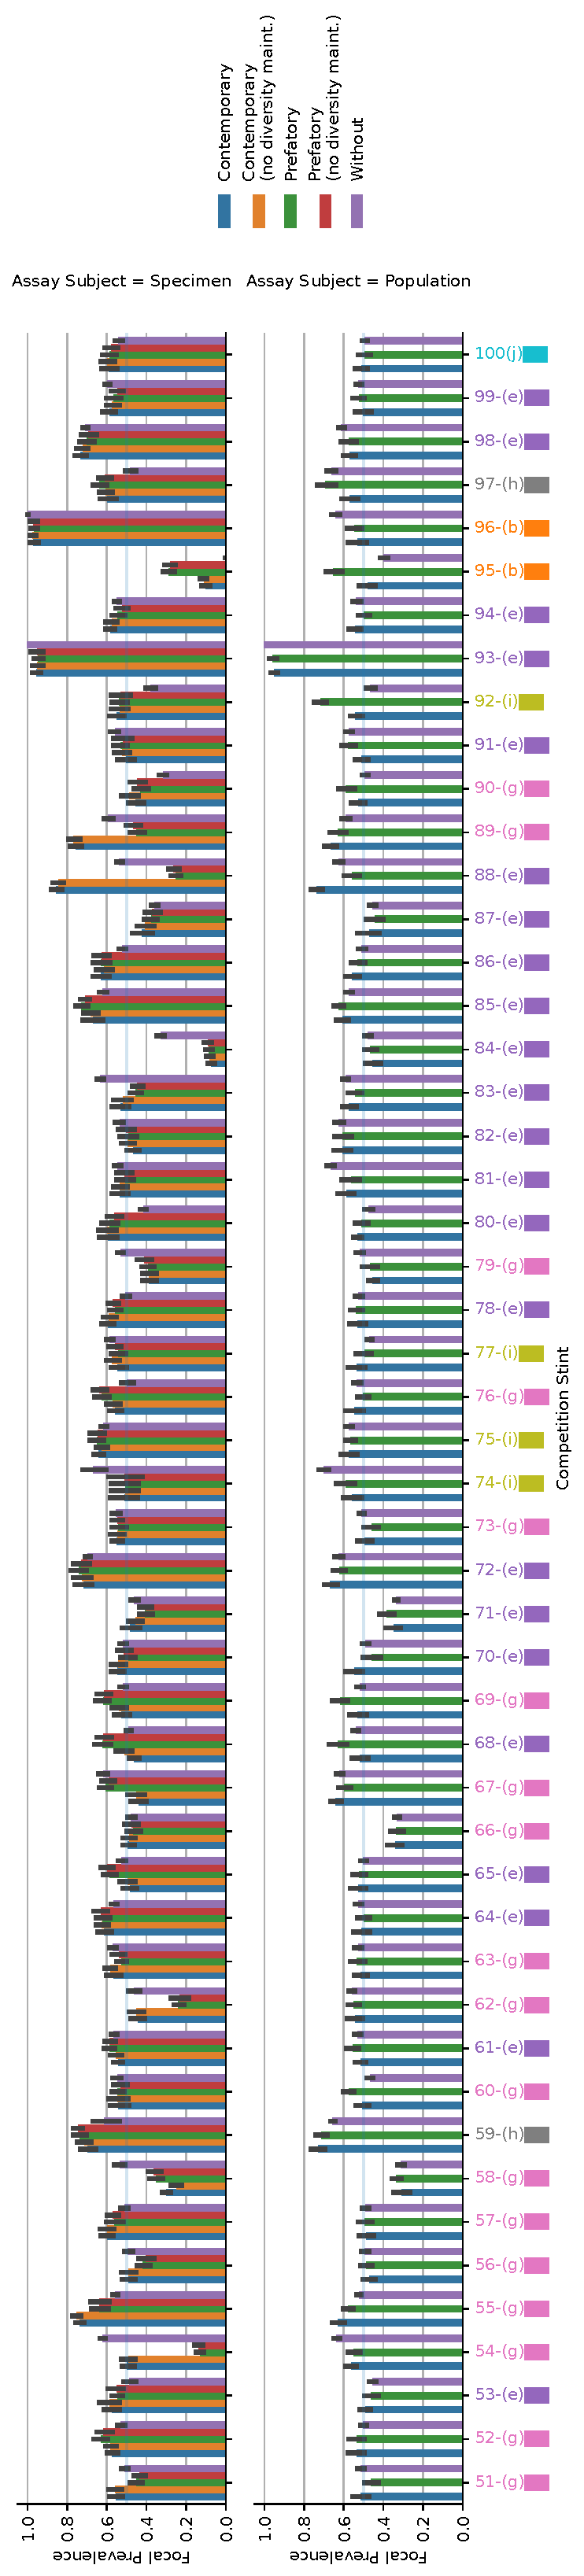
\includegraphics[width=\linewidth]{{submodule/dishtiny/binder/bucket=prq49/a=adaptation_assays+endeavor=16/teeplots/hue=biotic-background+stint=51-100+viz=facet-barplot+x=competition-stint+y=focal-prevalence+ext=}}

\caption{
TODO
}
\label{fig:mean_competition_prevalence_barplot}
\end{sidewaysfigure*}


\begin{figure*}
\centering

\begin{subfigure}{\textwidth}

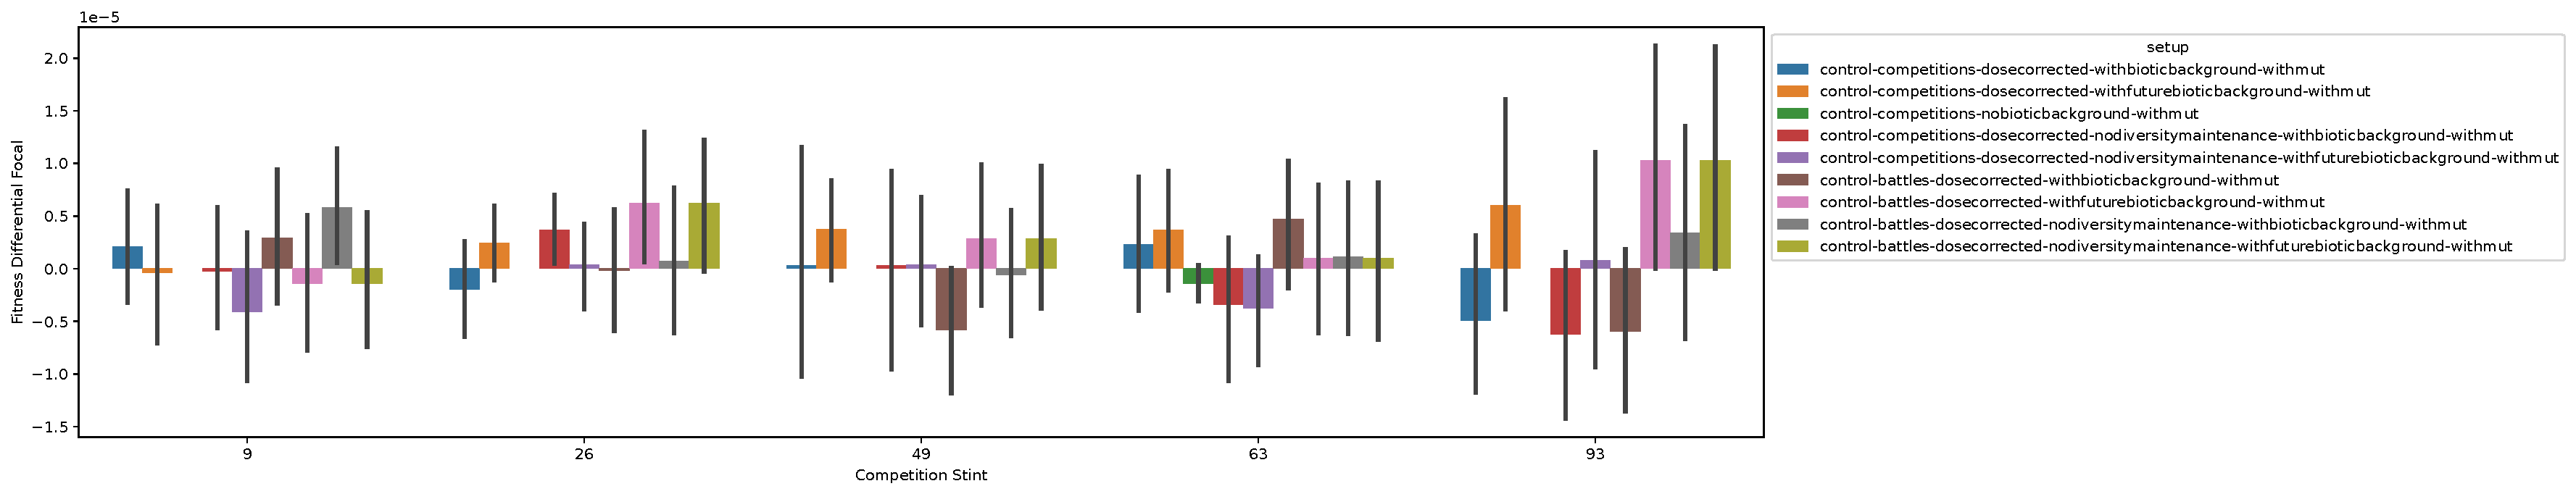
\includegraphics[width=\linewidth]{{submodule/dishtiny/binder/bucket=prq49/a=adaptation_assays+endeavor=16/teeplots/hue=setup+viz=barplot+x=competition-stint+y=fitness-differential-focal+ext=}}
\caption{
\footnotesize
Calculated fitness differential between competing strains based on population composition at the end of competition experiments.
Zero is neutral.
Error bars are 95\% confidence intervals.
}
\end{subfigure}

\begin{subfigure}{\textwidth}
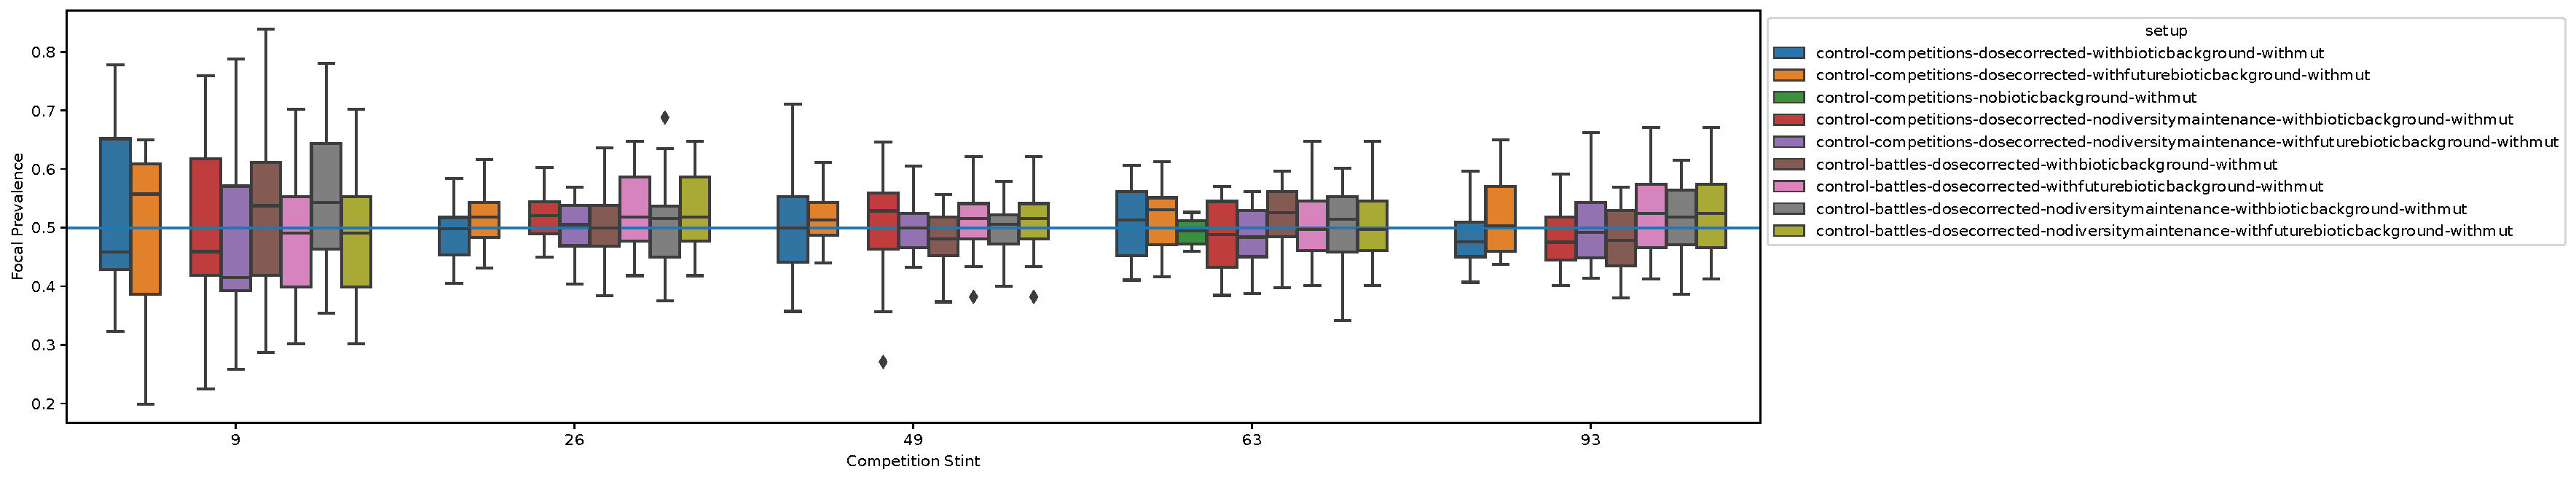
\includegraphics[width=\linewidth]{{submodule/dishtiny/binder/bucket=prq49/a=adaptation_assays+endeavor=16/teeplots/hue=setup+viz=boxplot+x=competition-stint+y=focal-prevalence+ext=}}
\caption{
\footnotesize
Fractional composition of focal population at the end of competition experiments.
A neutral outcome corresponds to even (0.5) composition, annotated with a horizontal line.
}
\end{subfigure}

\begin{subfigure}{\textwidth}
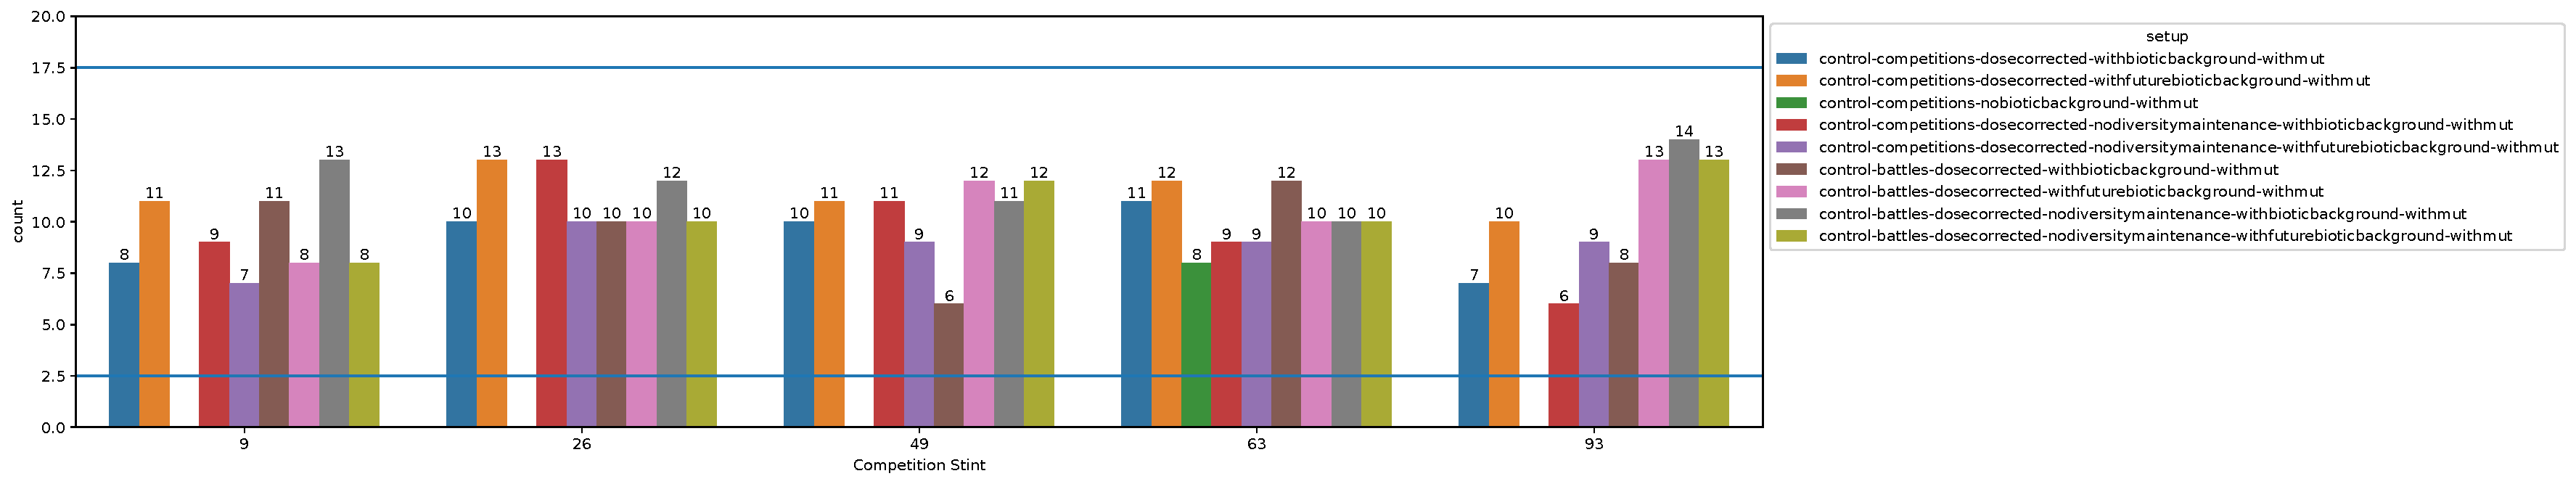
\includegraphics[width=\linewidth]{{submodule/dishtiny/binder/bucket=prq49/a=adaptation_assays+endeavor=16/teeplots/hue=setup+viz=countplot+x=competition-stint+ext=}}
\caption{
\footnotesize
Number competitions out of 20 won by first strain.
Ten competitions won corresponds to a perfectly neutral outcome.
Eighteen and more or two or less competitions won were considered to indidicate a significant fitness difference between strains.
These thresholds for significance annotated with horizontal lines.
}
\end{subfigure}

\caption{
\textbf{Control adaptation experiments for selected stints.}
\footnotesize
Control experiments were performed by competing two identical genomes or populations against each other with the contemporary biotic background, with the prefatory biotic background, or with no biotic background.
See Figure \ref{fig:adaptation_assay_cartoon} for summary of adaptation experiment design.
}
\label{fig:adaptation_control}
\end{figure*}


\begin{sidewaysfigure*}
\centering
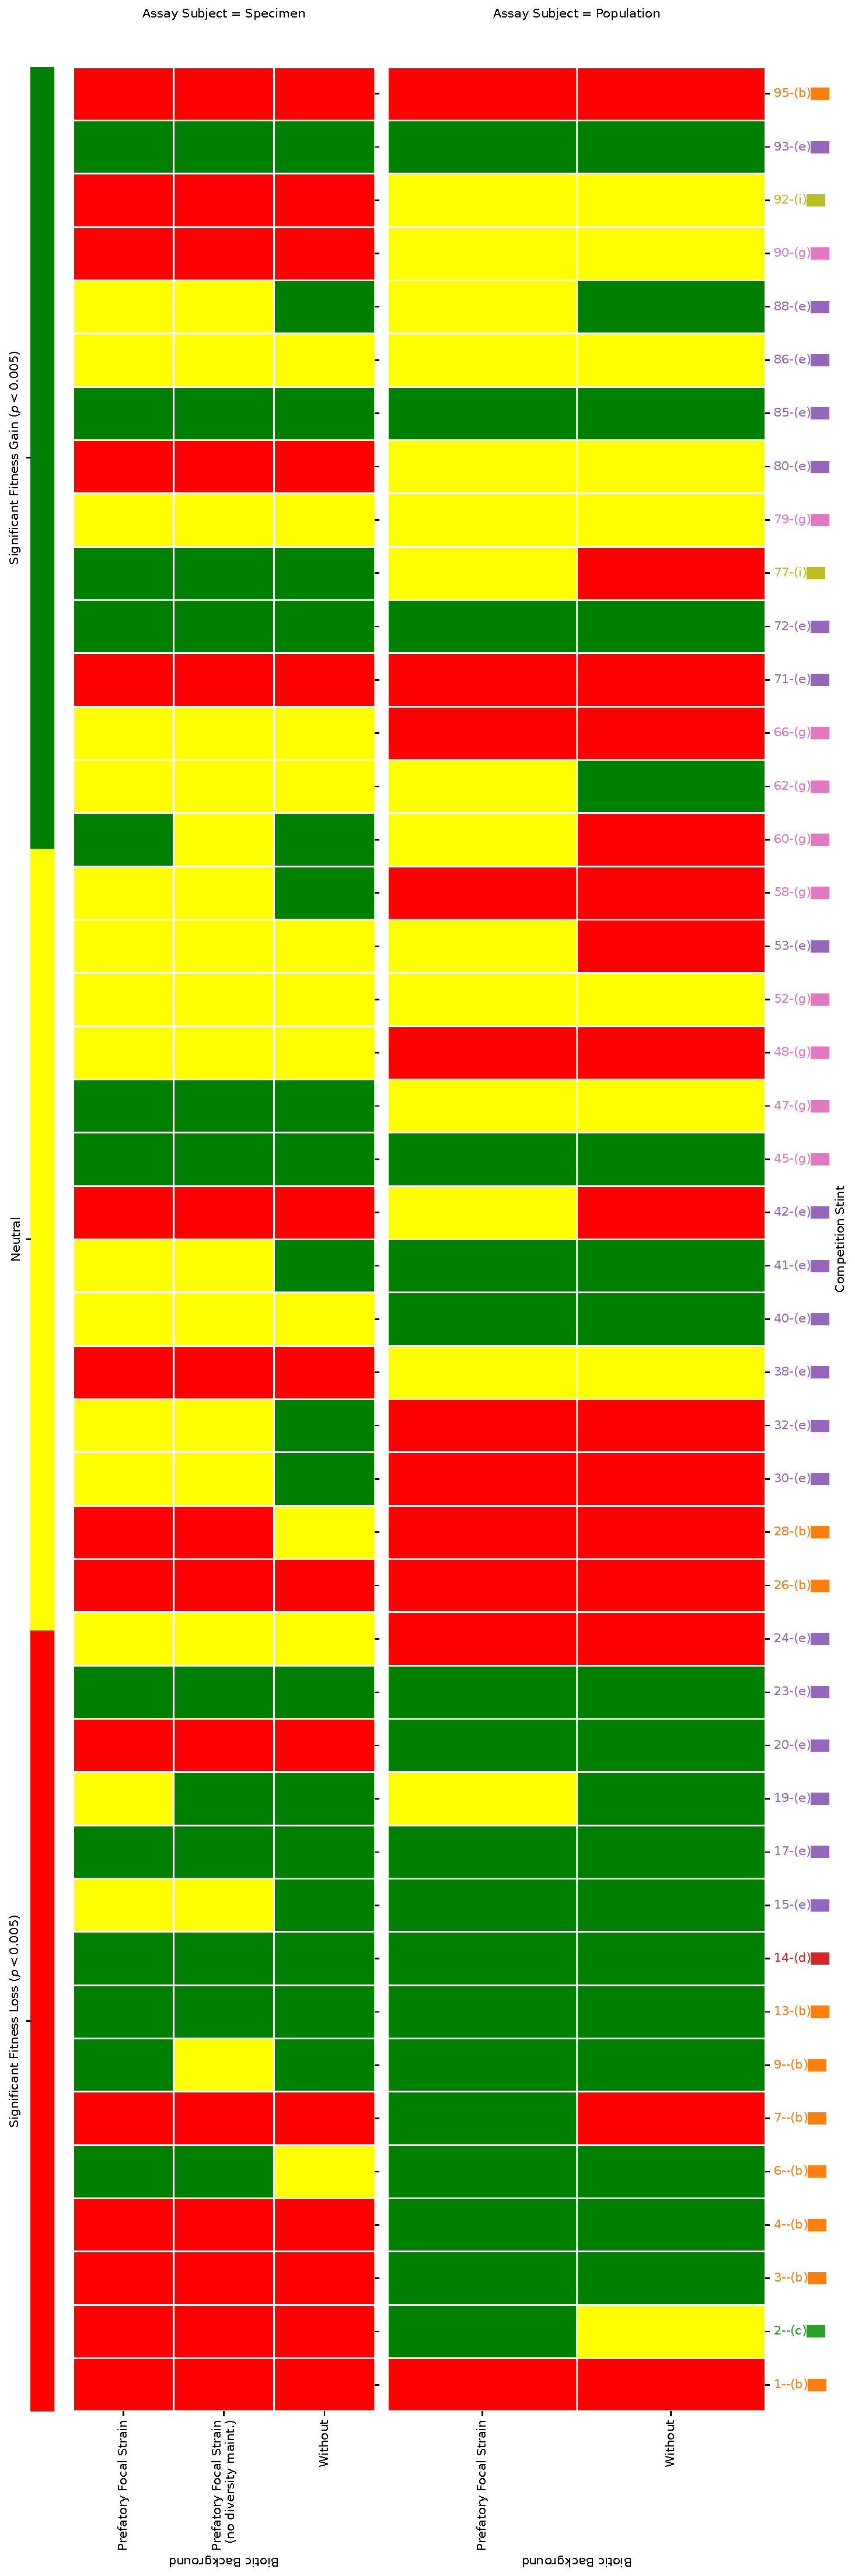
\includegraphics[width=\linewidth]{{submodule/dishtiny/binder/bucket=prq49/a=adaptation_assays+endeavor=16/teeplots/a=baselinecontrol+hue=fitness-gain-or-loss+viz=facet-heatmap+x=biotic-background+y=competition-stint+ext=}}

\caption{
Summary of biotic background control adaptation assay outcomes for sampled representative specimen (top) population-level adaptation (bottom).
Color coding and parentheticals of stint labels correspond to qualitative morph codes described in Table \ref{tab:morph_descriptions}.
See Figure \ref{fig:adaptation_assay_cartoon} for explanation of competition biotic backgrounds.
}
\label{fig:baseline_fitness_gain_or_loss}
\end{sidewaysfigure*}


\begin{figure*}
\centering

\begin{subfigure}{\textwidth}
\centering
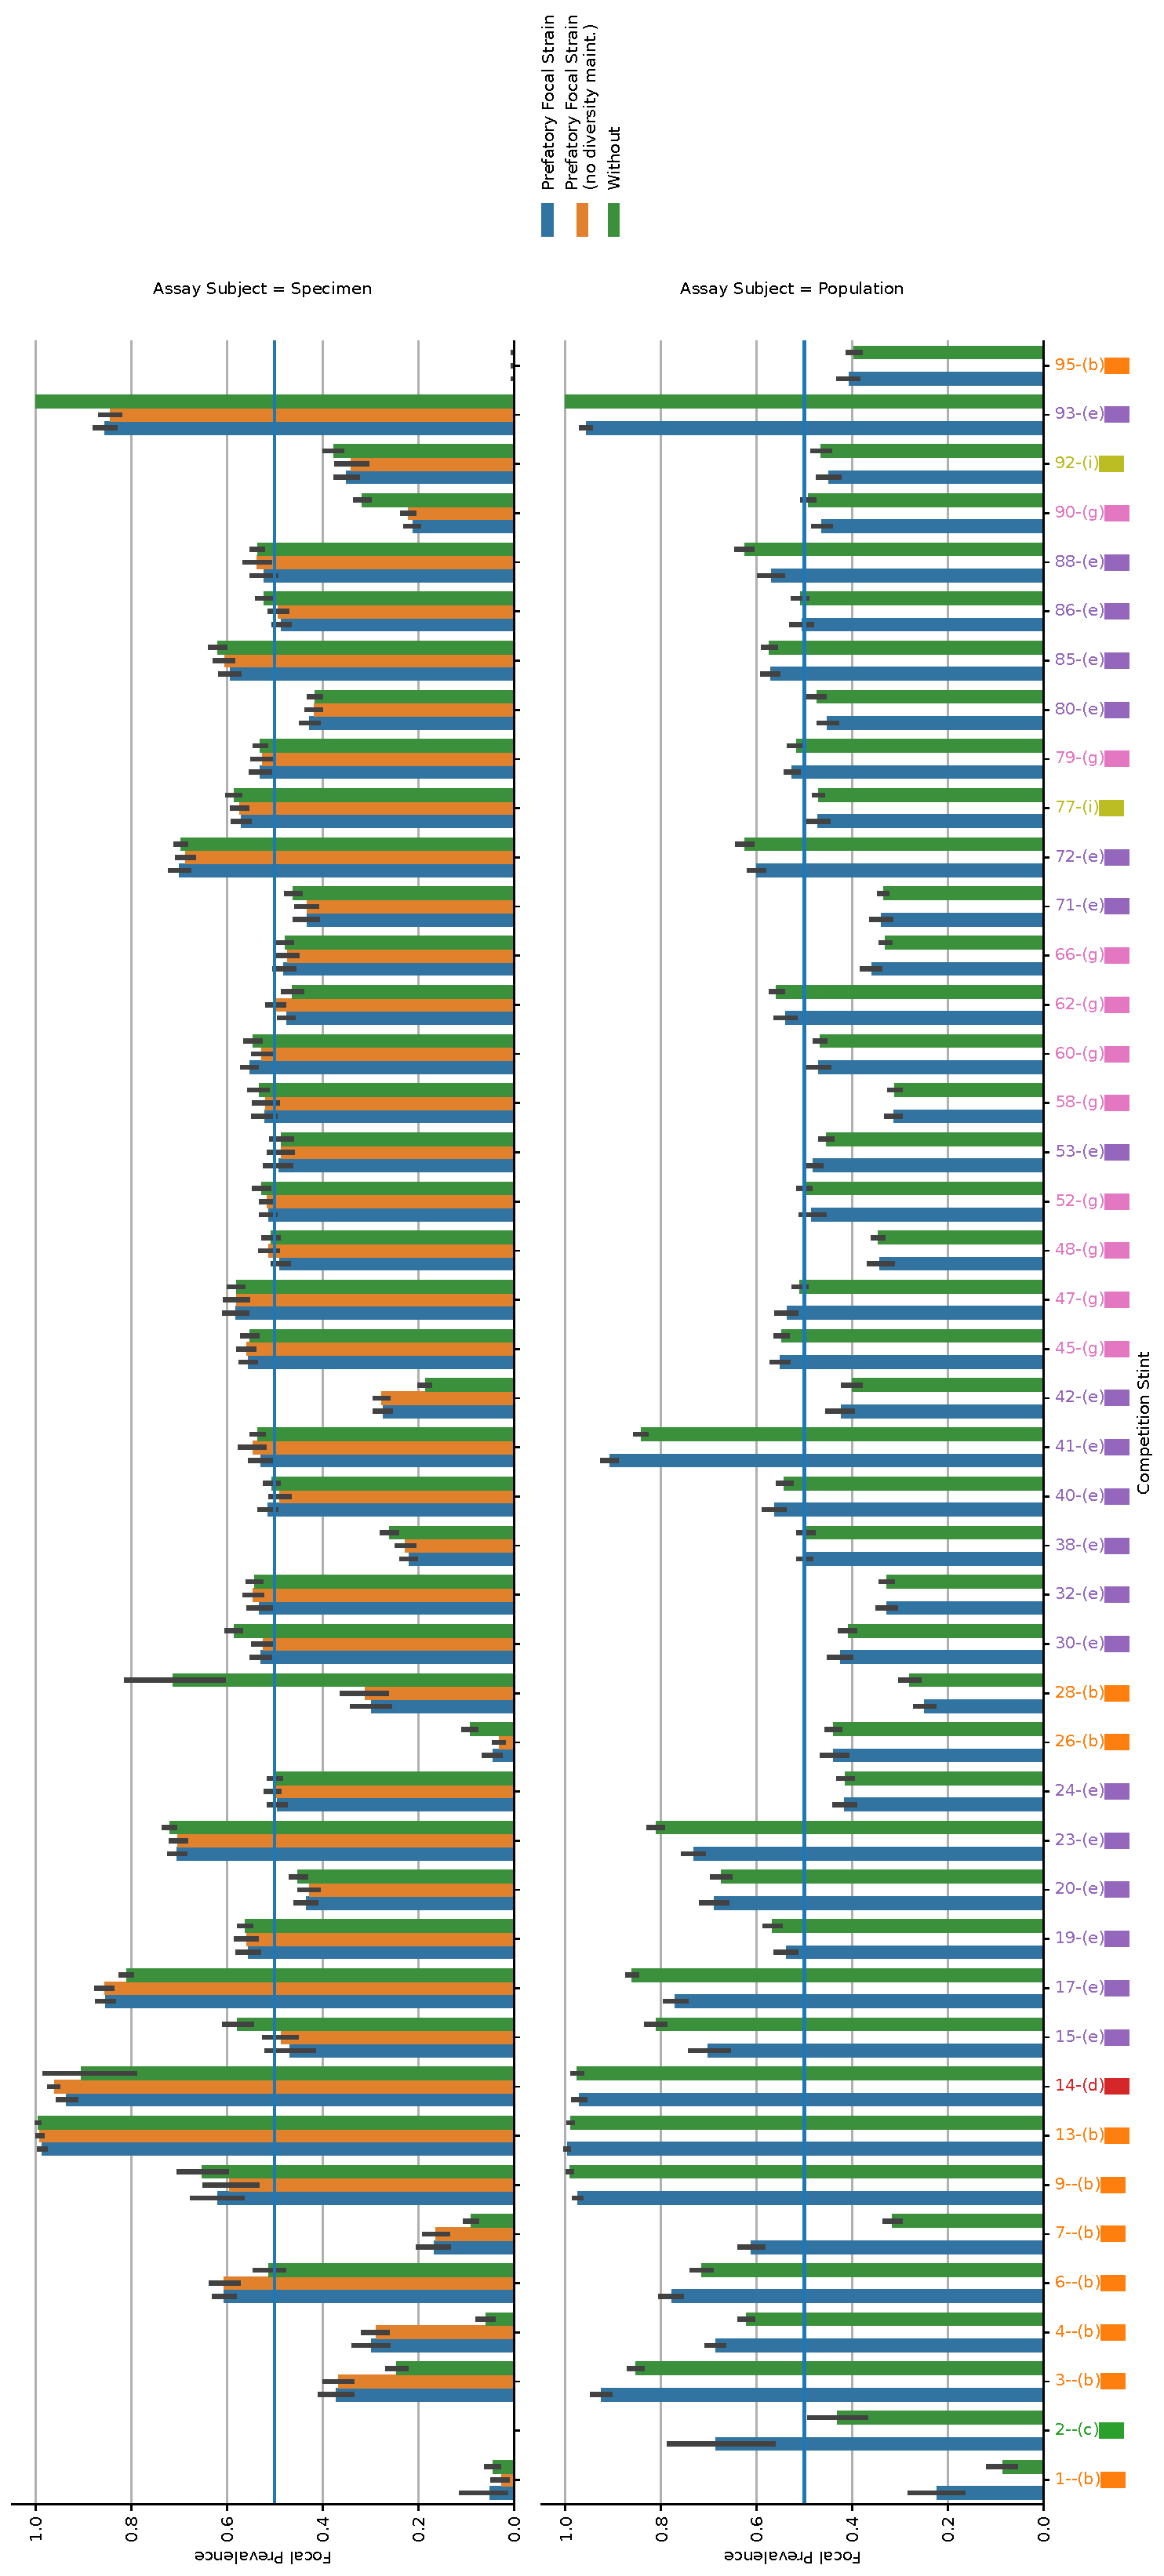
\includegraphics[width=0.7\linewidth]{{submodule/dishtiny/binder/bucket=prq49/a=adaptation_assays+endeavor=16/teeplots/a=baselinecontrol+hue=biotic-background+viz=facet-barplot+x=competition-stint+y=focal-prevalence+ext=}}
\caption{
Fractional composition of focal population at the end of competition experiments.
Zero is neutral.
Error bars are 95\% confidence intervals.
}
\end{subfigure}

\begin{subfigure}{\textwidth}
\centering
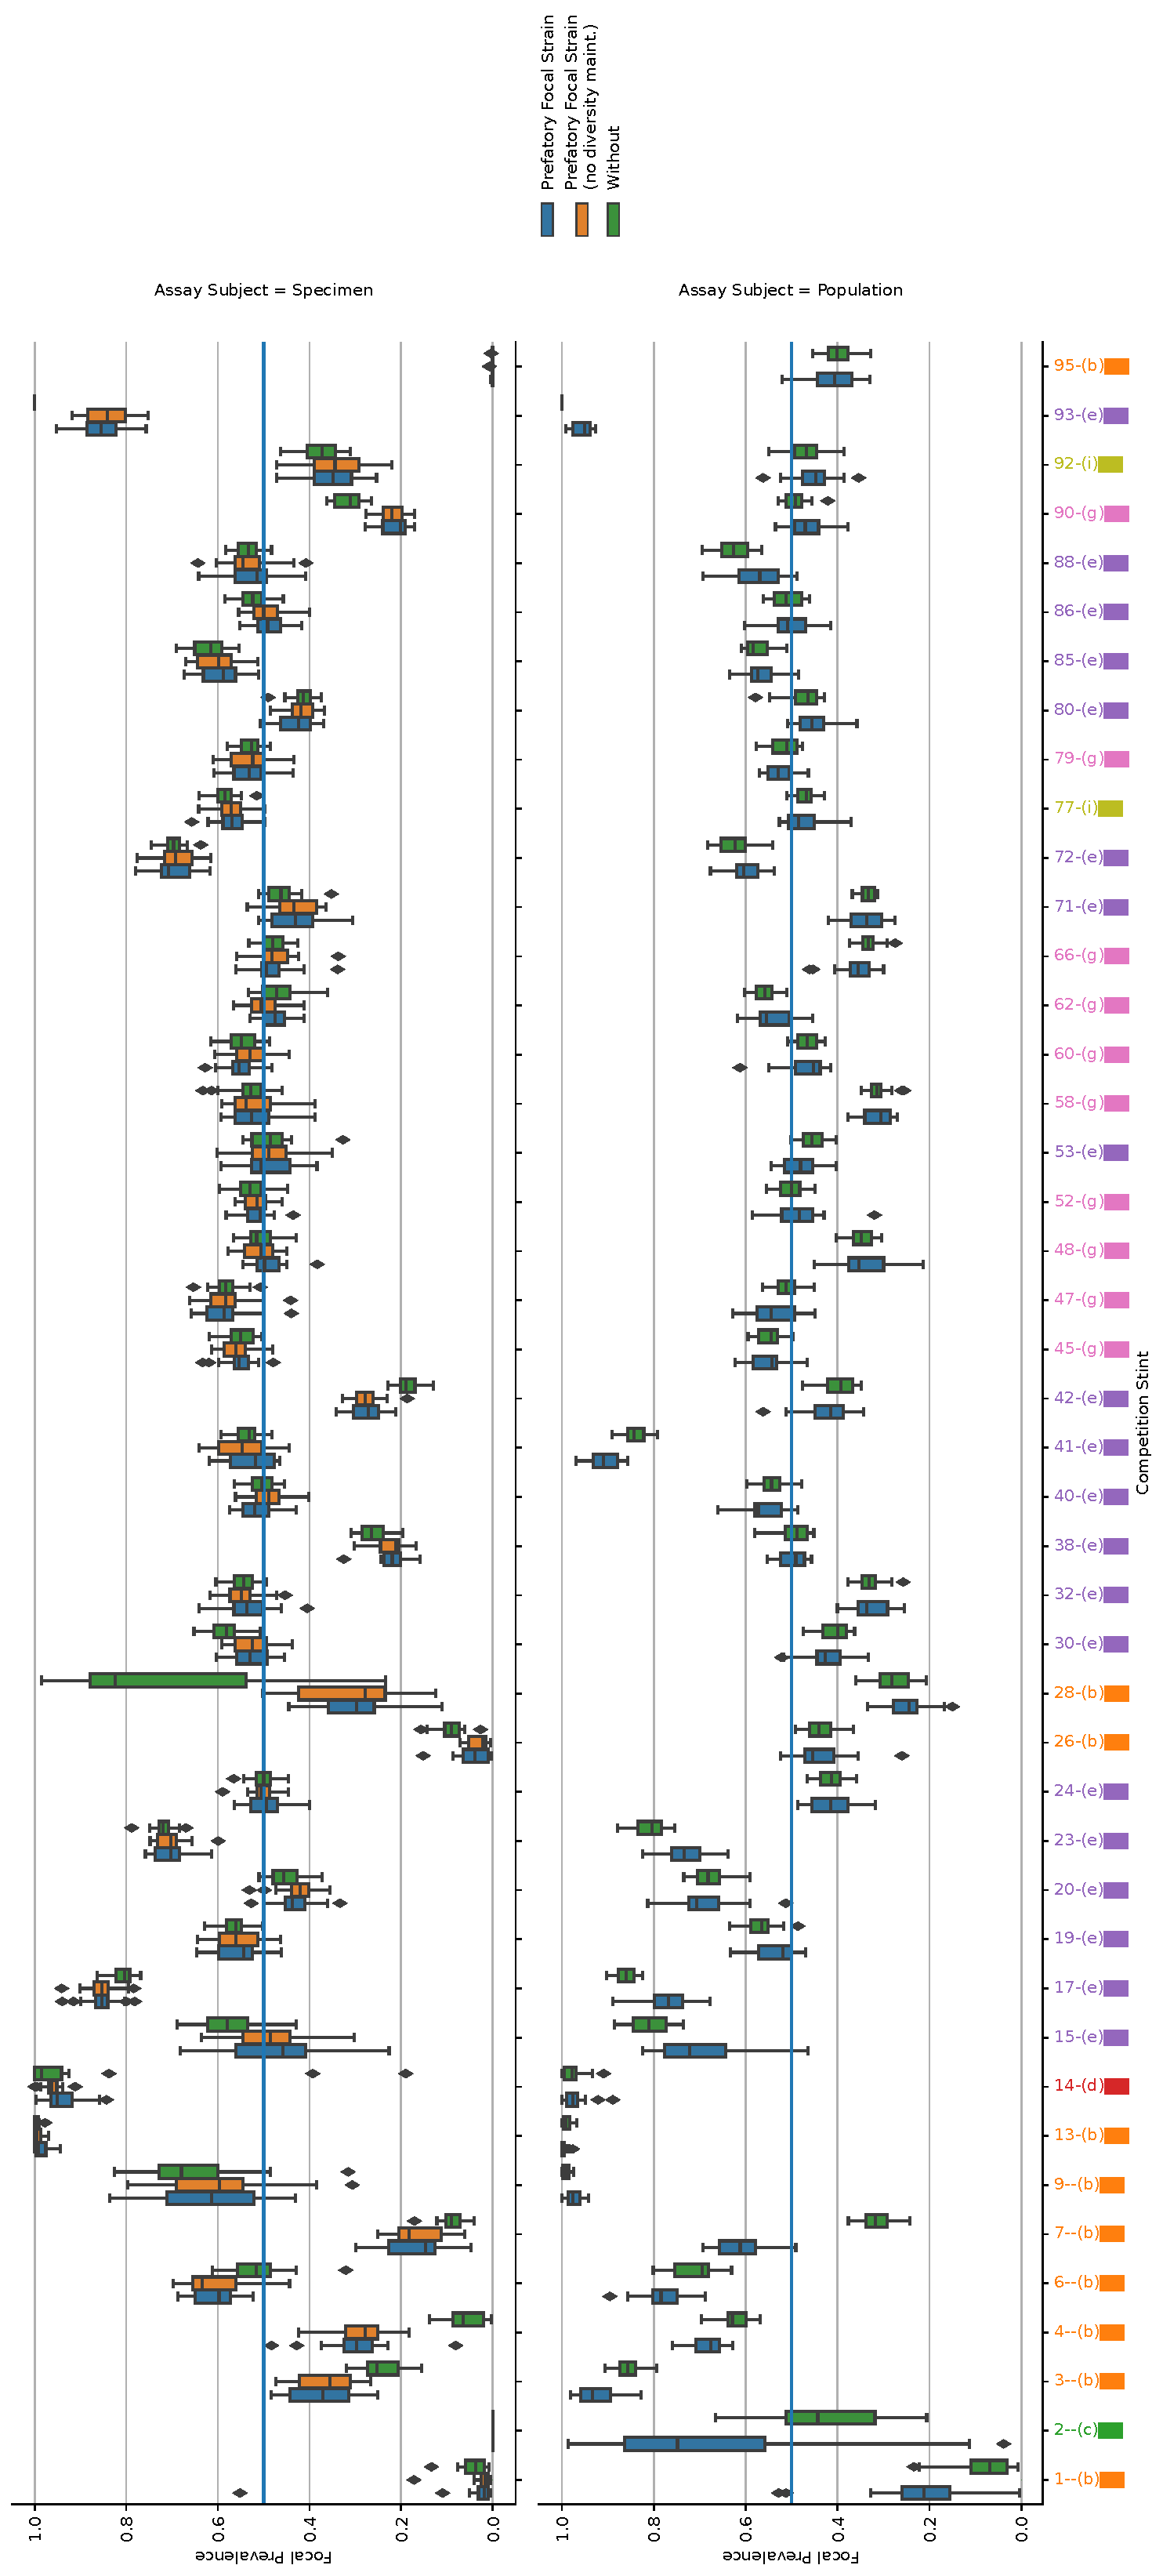
\includegraphics[width=0.7\linewidth]{{submodule/dishtiny/binder/bucket=prq49/a=adaptation_assays+endeavor=16/teeplots/a=baselinecontrol+hue=biotic-background+viz=facet-boxplot+x=competition-stint+y=focal-prevalence+ext=}}
\caption{
Fractional composition of focal population at the end of competition experiments.
A neutral outcome corresponds to even (0.5) composition, annotated with a horizontal line.
}
\end{subfigure}

\begin{subfigure}{\textwidth}
\centering
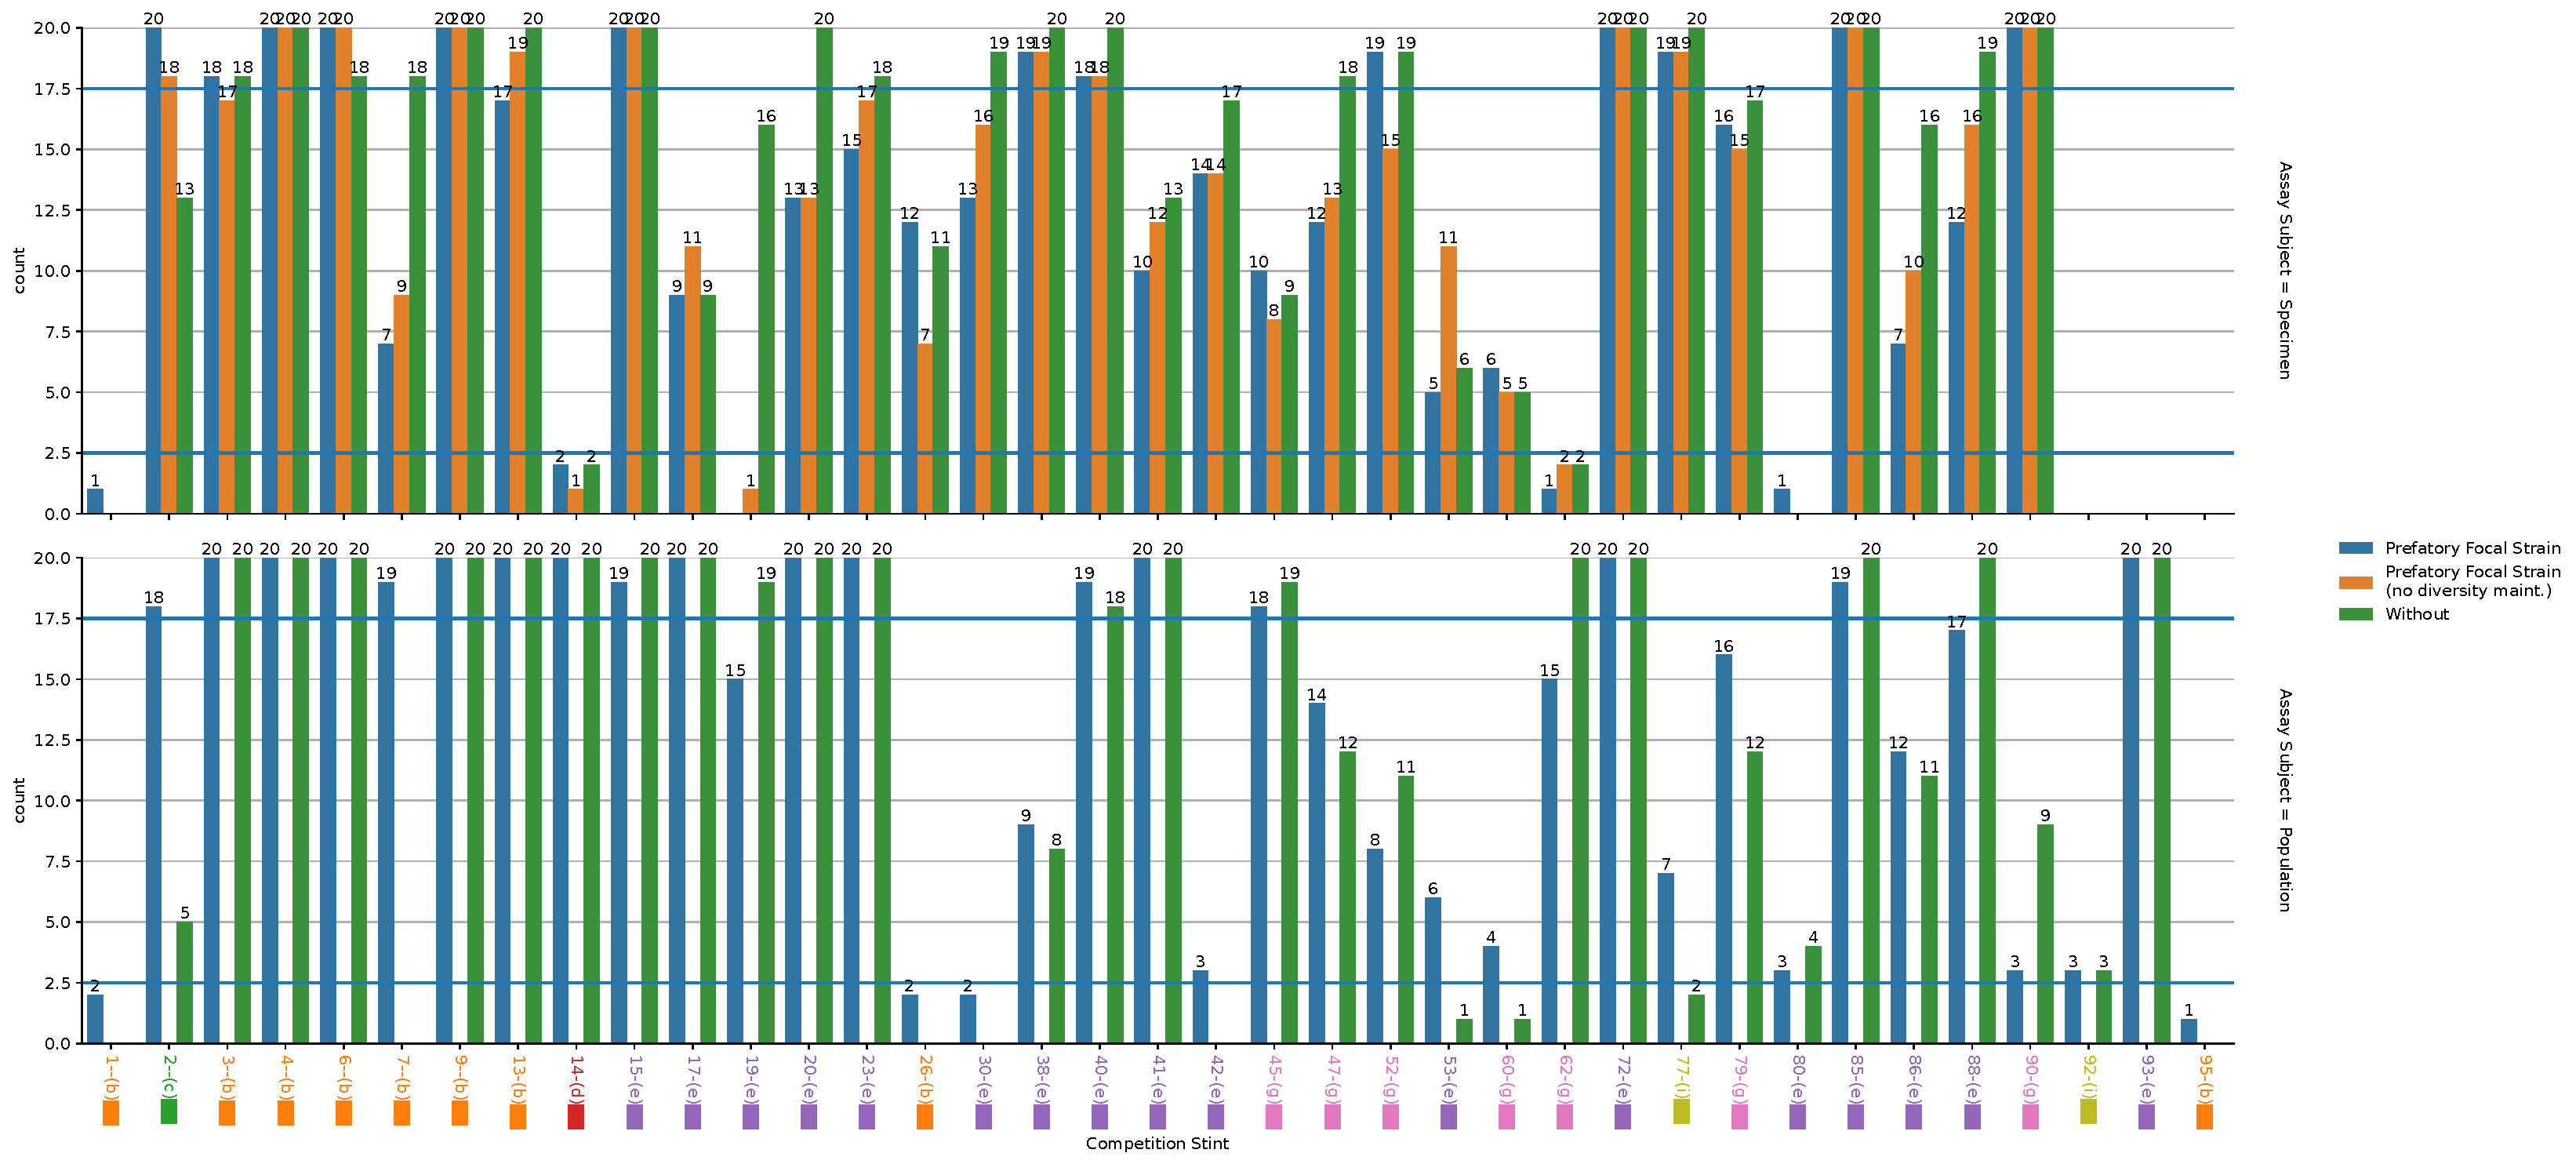
\includegraphics[width=0.7\linewidth]{{submodule/dishtiny/binder/bucket=prq49/a=adaptation_assays+endeavor=16/teeplots/a=baselinecontrol+hue=biotic-background+viz=facet-countplot+x=competition-stint+ext=}}
\caption{
Number competitions out of 20 won by first strain.
Ten competitions won corresponds to a perfectly neutral outcome.
Eighteen and more or two or less competitions won were considered to indicate a significant fitness difference between strains.
These thresholds for significance annotated with horizontal lines.
}
\end{subfigure}

\caption{
Biotic background control adaptation experiments for selected stints.
Biotic background control experiments were performed by substituting the baseline competitor for the biotic background.
See Figure \ref{fig:adaptation_assay_cartoon} for summary of adaptation experiment design.
}
\label{fig:baseline_adaptation_control}
\end{figure*}


\begin{figure}

\begin{subfigure}{\linewidth}

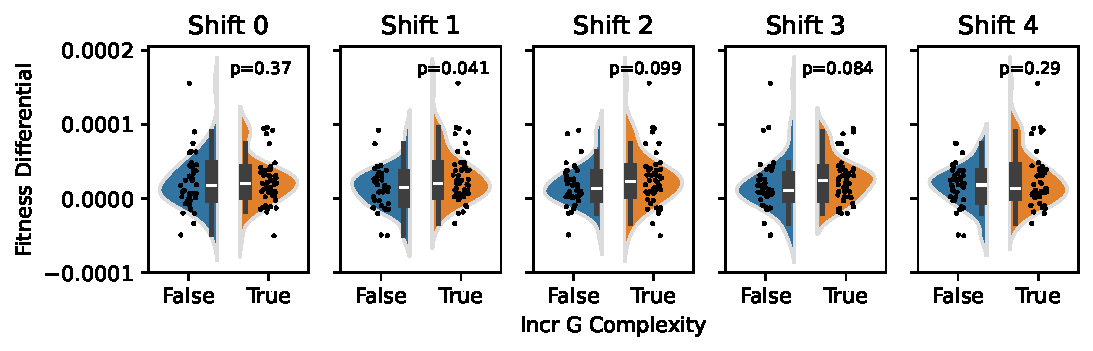
\includegraphics[width=\linewidth]{binder-2025-08-28-complexity-adaptation/binder/teeplots/2025-08-28-complexity-adaptation/how=shift+sign=-1+viz=subplots+ext=.pdf}
\caption{fitness differential value at forward-looking offset, "shift" corresponding to offset size}

\end{subfigure}

\vspace{2ex}

\begin{subfigure}{\linewidth}

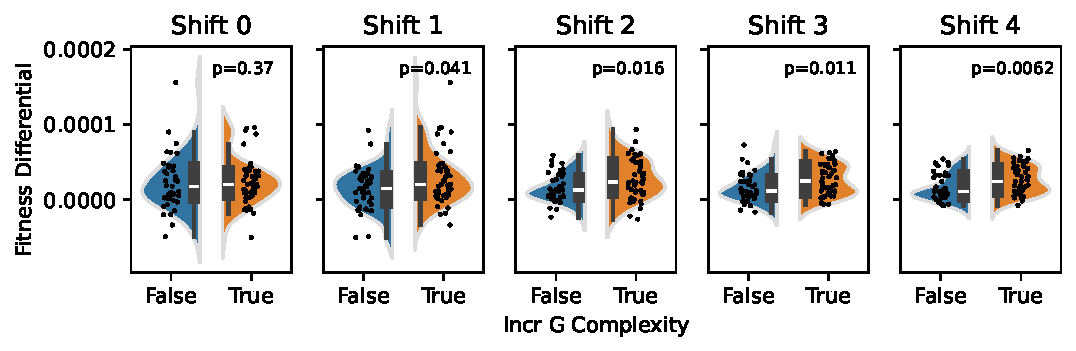
\includegraphics[width=\linewidth]{binder-2025-08-28-complexity-adaptation/binder/teeplots/2025-08-28-complexity-adaptation/how=rollingmean+sign=-1+viz=subplots+ext=.pdf}
\caption{fitness differential mean over forward-looking window, "shift" corresponding to window size}

\end{subfigure}

\vspace{1ex}

\caption{
\textbf{Backwards-looking control for Figure \ref{fig:potentiate}.}
Comparisons find no backwards-looking association between complexity and fitness gains (i.e., fitness gains driving subsequent complexity increase).
}
\label{fig:potentiate-control}

\end{figure}


\begin{figure*}

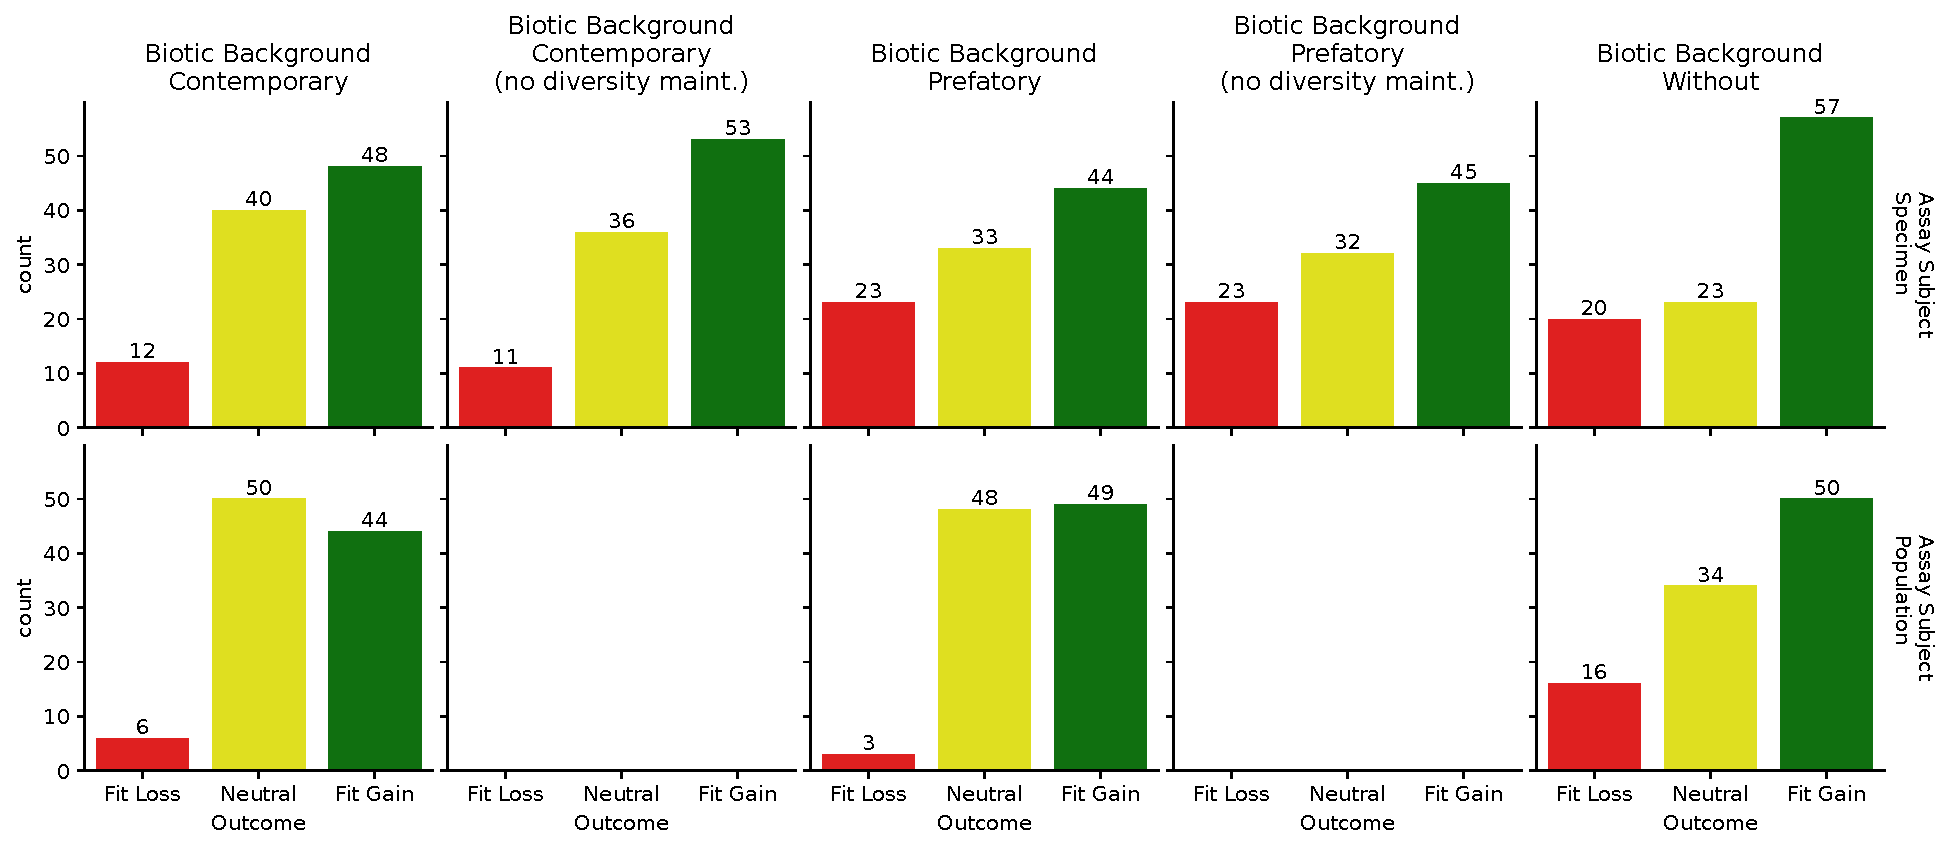
\includegraphics[width=\linewidth]{{submodule/dishtiny/binder/bucket=prq49/a=adaptation_assays+endeavor=16/teeplots/col=biotic-background+kind=count+row=assay-subject+viz=barlabel-catplot+x=outcome+ext=}}

\caption{
TODO
}
\label{fig:outcome_count_distns}
\end{figure*}


\begin{figure*}
\centering
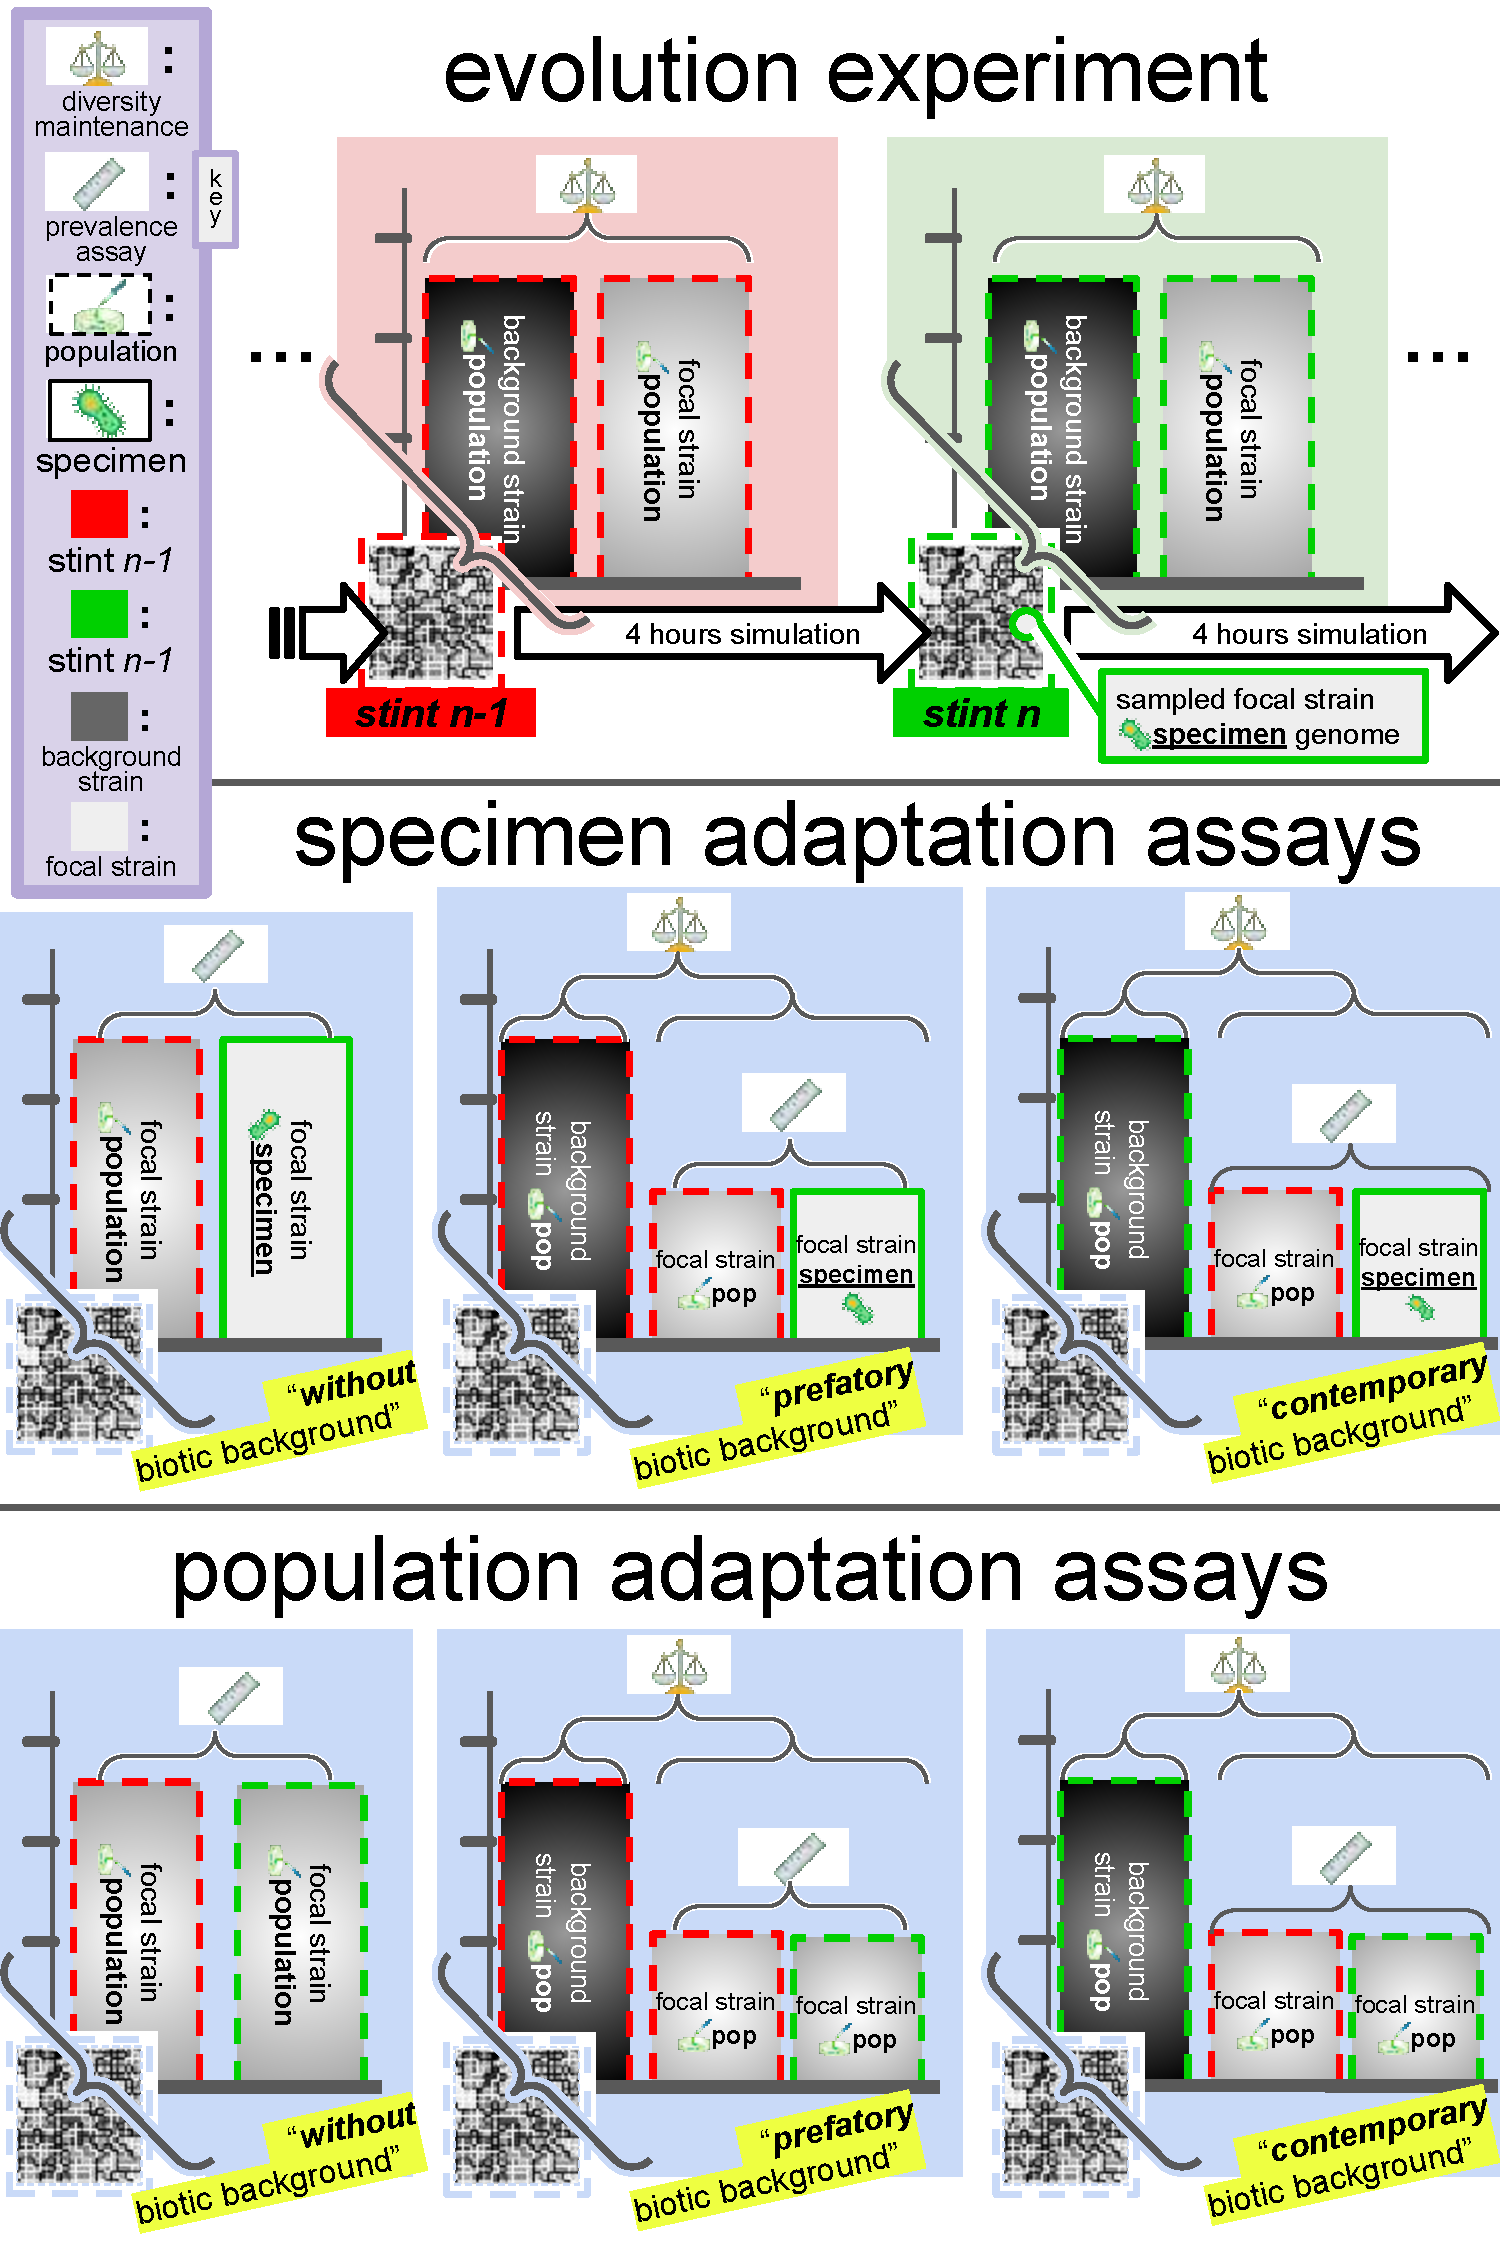
\includegraphics[width=0.5\linewidth]{{img/adaptation-assay-cartoon}}

\caption{
Detail of adaptation assay design.
Top panel shows progress of original evolutionary experiment over one stint.
A diversity maintenance procedure was used to ensure long-term coexistence of a least two strains over the course of the experiment by penalizing any strain that occupied more than half of thread-local population space.
A ``focal strain'' was arbitrarily chosen for study; we refer to the other strain as the ``background strain.''
Adaptation assays in lower panels measure fitness change over the course of that stint through against the population from the preceding stint.
The middle panel shows measurement of adaptation of the representative specimen that was sampled for analysis at each stint.
The bottom panel shows measurement of the adaptation of the entire focal strain population at each stint.
Competitors were mixed in even proportion into the environment.
Bar heights represent initial relative proportions of assay participants at the beginning of the competition.
Adaptation was measured by measuring change in population composition over a 10 minute competition window.
We call this measurement of population composition change a ``prevalence assay''.
Competition experiments were performed absent the background strain, with the background strain population from the preceding stint, or with the background strain population from the current stint --- shown separately in each panel.
}
\label{fig:adaptation_assay_cartoon}
\end{figure*}


\begin{sidewaysfigure*}
\thisfloatpagestyle{mylandscape}%
\rotatesidewayslabel%
\centering

\begin{subfigure}[t]{0.32\textwidth}
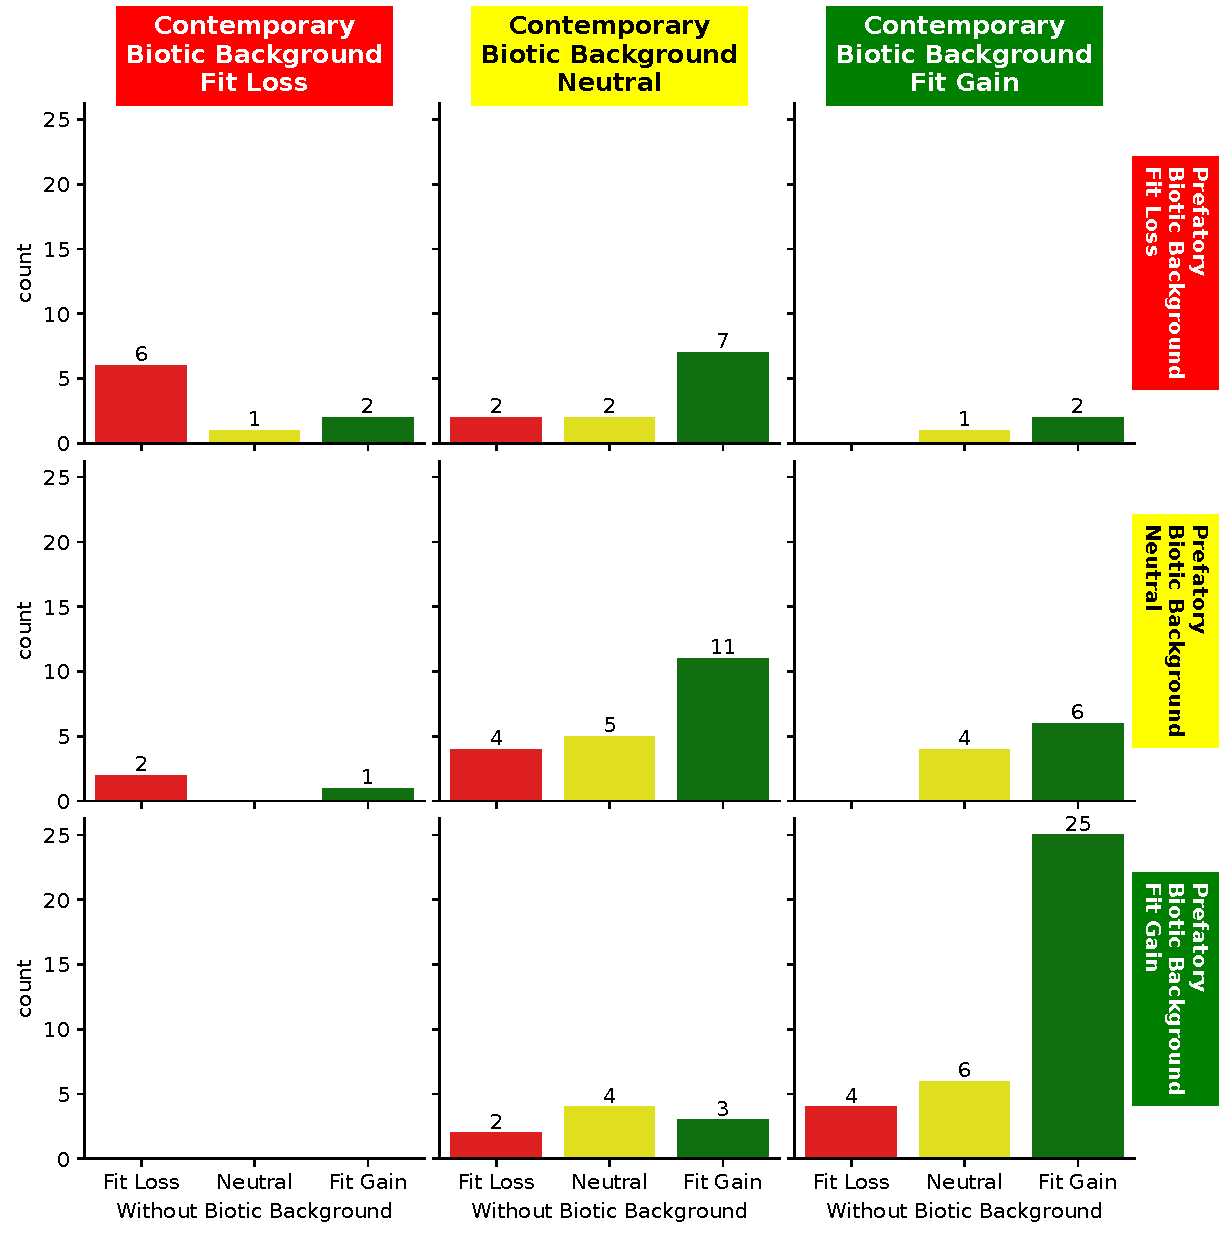
\includegraphics[width=\linewidth]{{submodule/dishtiny/binder/bucket=prq49/a=adaptation_assays+endeavor=16/teeplots/assay-subject=Specimen+col=contemporary-biotic-background+kind=count+row=prefatory-biotic-background+viz=barlabel-catplot+x=without-biotic-background+ext=}}
\caption{Joint distribution of adaptation assay on representative specimen from focal strain over biotic backgrounds, with diversity maintenance during competition.}
\label{fig:outcome_count_joint_distns:specimen_with_dm}
\end{subfigure}%
\hfill%
\begin{subfigure}[t]{0.32\textwidth}
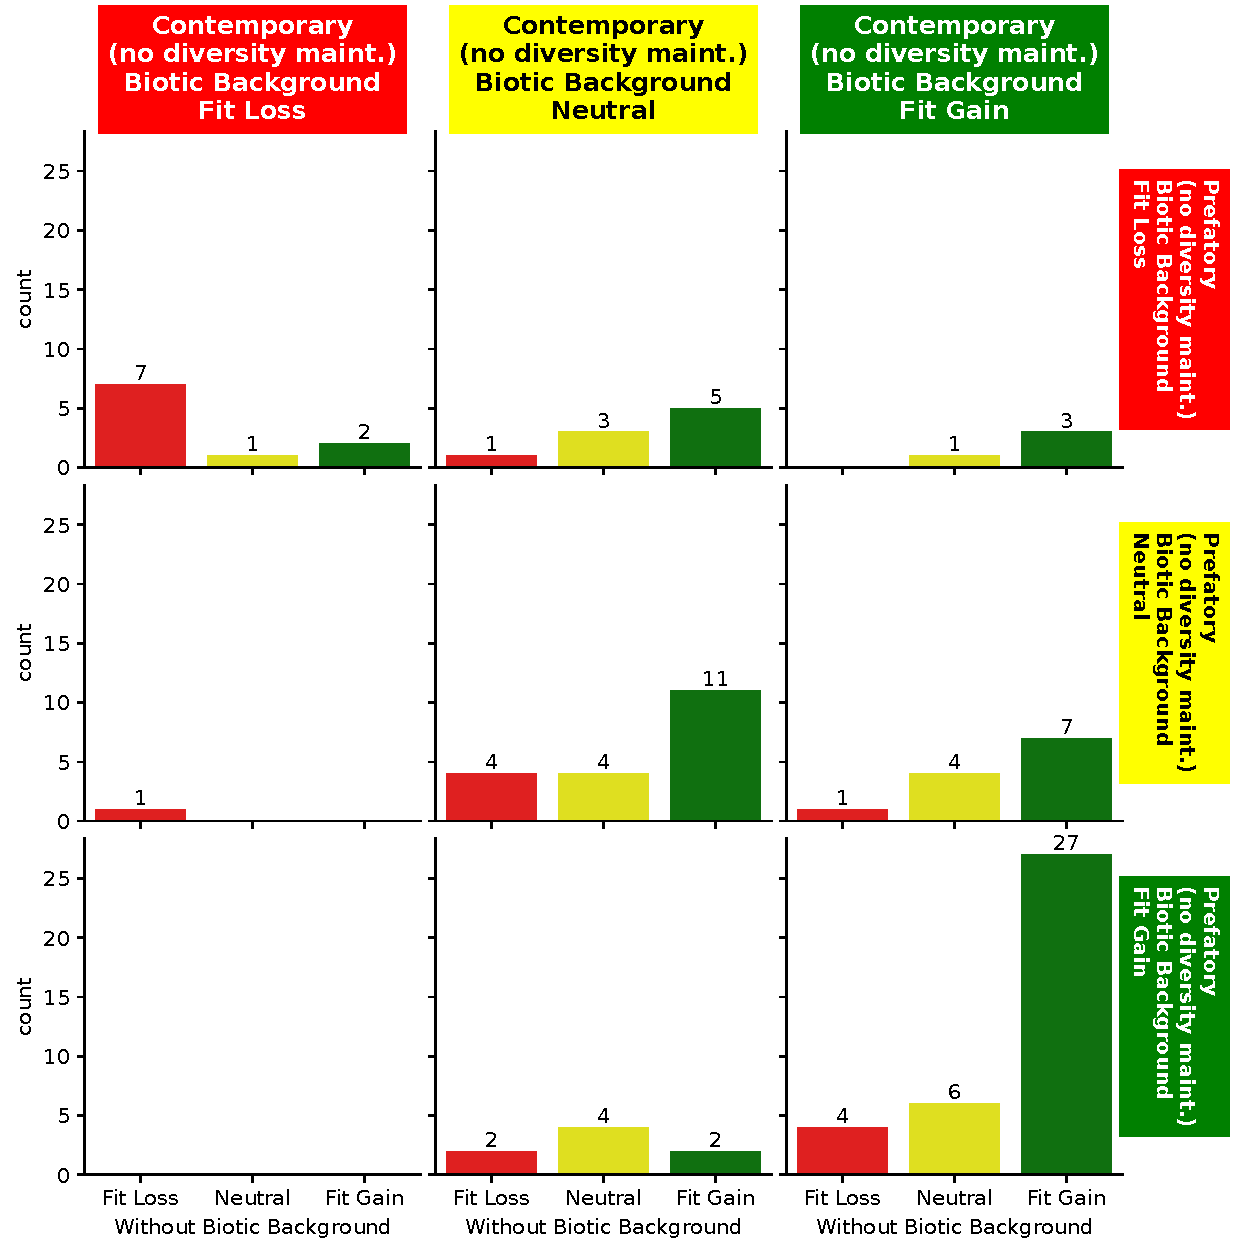
\includegraphics[width=\linewidth]{{submodule/dishtiny/binder/bucket=prq49/a=adaptation_assays+endeavor=16/teeplots/assay-subject=Specimen+col=contemporary-no-diversity-maint-biotic-background+kind=count+row=prefatory-no-diversity-maint-biotic-background+viz=barlabel-catplot+x=without-biotic-background+ext=}}
\caption{Joint distribution of adaptation assay on representative specimen from focal strain over biotic backgrounds, with diversity maintenance disabled during competition.}
\label{fig:outcome_count_joint_distns:specimen_no_dm}
\end{subfigure}%
\hfill%
\begin{subfigure}[t]{0.32\textwidth}
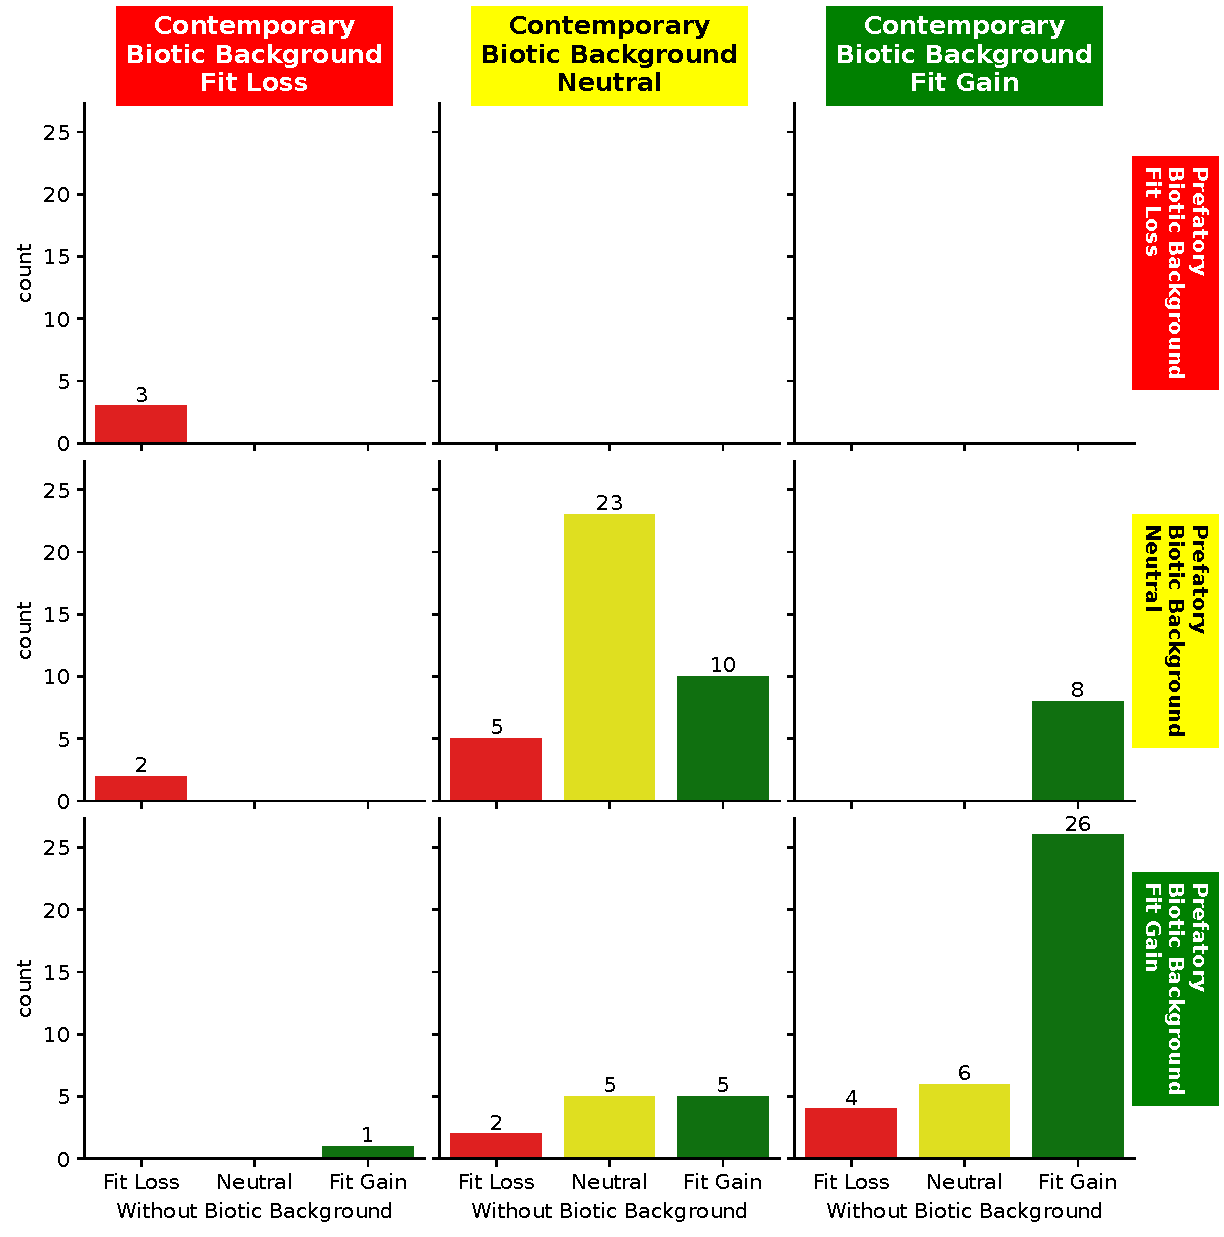
\includegraphics[width=\linewidth]{{submodule/dishtiny/binder/bucket=prq49/a=adaptation_assays+endeavor=16/teeplots/assay-subject=Population+col=contemporary-biotic-background+kind=count+row=prefatory-biotic-background+viz=barlabel-catplot+x=without-biotic-background+ext=}}
\caption{Joint distribution of adaptation assay on focal strain population over biotic backgrounds, with diversity maintenance during competition.}
\label{fig:outcome_count_joint_distns:population}
\end{subfigure}


\caption{
\textbf{Effect of biotic background on adaptation assay outcomes.}
\footnotesize
Joint distribution of adaptation assay outcomes across biotic backgrounds.
For each adaptation assay, three outcomes were possible: significant fitness gain, significant fitness loss, or no significant fitness change (``neutral'').
Significance cutoff $p < 0.005$ was used.
A fitness loss --- color-coded red --- corresponds to winning 2 or fewer competitions out of 20 against the preceding stint's focal strain population.
A fitness gain --- color-coded green --- corresponds to winning 18 or more competitions out of 20 against the preceding stint's focal strain population.
Neutral fitness outcomes are color-coded yellow.
Outcome counts are accumulated over experiments from stint 1 through stint 100.
Counts in each subfigure therefore sum to 100.
Column position in facet grid indicates outcome with contemporary biotic background, row position indicates outcome with prefatory biotic background, and bar color and $x$ position indicates outcome without biotic background.
See Figure \ref{fig:adaptation_assay_cartoon} for explanation of competition biotic backgrounds.
See Figure \ref{fig:with_vs_without_diversity_maintenance} for detail on joint distribution of outcomes with and without diversity maintenance, which were mostly identical.
}
\label{fig:outcome_count_joint_distns}
\end{sidewaysfigure*}


\begin{figure*}
\centering
\includegraphics[width=0.8\linewidth]{{submodule/dishtiny_event_tag_phylogenetics/teeplots/ladderized_parsimony_tree_no_outliers/viz=draw+ext=}}

\caption{
\textbf{Estimated phylogeny of sampled focal strain representatives.}
\footnotesize
Phylogeny constructed using parsimony algorithm based on genome tag bitstring content \citep{cock2009biopython}.
Each leaf node corresponds to a sampled representative.
Representatives from stints 0 and 1, which share no common ancestry with representatives from other stints, are excluded.
Numbers refer to stint that each representative was sampled from.
Color coding and parentheticals of stint labels correspond to qualitative morph codes described in Table \ref{tab:morph_descriptions}.
}
\label{fig:phylo_parsimony_tree}
\end{figure*}


\begin{figure*}
\centering
\captionsetup[subfigure]{font=footnotesize}
\begin{subfigure}[t]{0.49\textwidth}
\includegraphics[width=\linewidth]{{submodule/dishtiny/binder/bucket=prq49/a=adaptation_assays+endeavor=16/teeplots/assay-subject=Specimen+hue=prefatory-no-diversity-maint-biotic-background+kind=count+viz=barlabel-catplot+x=prefatory-biotic-background+ext=}}
\caption{prefatory biotic background outcomes with and without diversity maintenance}
\end{subfigure}%
\hfill%
\begin{subfigure}[t]{0.49\textwidth}
\includegraphics[width=\linewidth]{{submodule/dishtiny/binder/bucket=prq49/a=adaptation_assays+endeavor=16/teeplots/assay-subject=Specimen+hue=contemporary-no-diversity-maint-biotic-background+kind=count+viz=barlabel-catplot+x=contemporary-biotic-background+ext=}}
\caption{contemporary biotic background outcomes with and without diversity maintenance}
\end{subfigure}

\caption{
\textbf{Effect of diversity maintenance on adaptation assays with biotic background.}
\footnotesize
Joint distribution of competition experiments performed under biotic background conditions with diversity maintenance enabled and disabled.
Color coding denotes outcome without diversity maintenance and $x$ position denotes outcome with diversity maintenance.
Note that both plots above show distributions for adaptation assays on representative specimens.
Competition experiments without diversity maintenance were not performed for population-level adaptation.
See Figure \ref{fig:adaptation_assay_cartoon} for explanation of competition biotic backgrounds.
}
\label{fig:with_vs_without_diversity_maintenance}
\end{figure*}


\begin{sidewaysfigure*}
\thisfloatpagestyle{mylandscape}%
\rotatesidewayslabel%
\centering
\includegraphics[width=\linewidth]{{submodule/dishtiny/binder/bucket=prq49/a=adaptation_assays+endeavor=16/teeplots/hue=fitness-gain-or-loss+viz=facet-heatmap+x=biotic-background+y=competition-stint+ext=}}

\caption{
\textbf{Adaptation Assay Outcomes.}
\footnotesize
Summary of adaptation assay outcomes for sampled representative specimen (top) and population-level adaptation (bottom).
Color coding and parentheticals of stint labels correspond to qualitative morph codes described in Table \ref{tab:morph_descriptions}.
See Figure \ref{fig:adaptation_assay_cartoon} for explanation of competition biotic backgrounds.
}
\label{fig:fitness_gain_or_loss}
\end{sidewaysfigure*}


\begin{sidewaysfigure*}
\centering
\includegraphics[width=\linewidth]{{submodule/dishtiny/binder/bucket=prq49/a=adaptation_assays+endeavor=16/teeplots/hue=symlog-median-fitness-differential+viz=facet-heatmap+x=biotic-background+y=competition-stint+ext=}}

\caption{
TODO
}
\label{fig:median_fitness_differential_symlog}
\end{sidewaysfigure*}


\begin{figure}

\includegraphics[width=\linewidth]{{plots/fitness/bucket=prq49+cat=morph+endeavor=16+transform=filter-Series-16005+viz=letterscatter-vline+x=stint+y=mean-doubling-time-growth-rate+ext=}}

\caption{Growth rate estimated from doubling time experiments, measuring time for a monoculture to grow from 0.25 maximum population size to 0.5 maximum population size.}
\label{fig:doubling_time}

\end{figure}


% \pragmaonce

% adapted from https://www.overleaf.com/learn/latex/Commands
\providecommand{\dissertationonly}[1]{%
% adapted from https://tex.stackexchange.com/a/33577
\ifdefined\DISSERTATION%
#1%
\else%
\fi
}

\begin{figure*}
\dissertationonly{\captionsetup[subfigure]{font=scriptsize}}
\dissertationonly{\captionsetup{font=footnotesize}}
\begin{subfigure}[t]{0.49\textwidth}

\includegraphics[width=\linewidth]{{plots/cardinal_interface_complexity/bucket=prq49+cat=morph+endeavor=16+transform=filter-Series-16005+viz=letterscatter+x=stint+y=cardinal-interface-complexity+ext=}}

\caption{Cardinal processor interface complexity, the total number of distinct interactions between a virtual CPU controlling cell behavior and its surroundings that contribute to fitness.
(Sum of Figures \labelcref{fig:interface_complexity:extrospective_interface_complexity,fig:interface_complexity:introspective_interface_complexity,fig:interface_complexity:writable_interface_complexity,fig:interface_complexity:intermessage_interface_complexity,fig:interface_complexity:intramessage_interface_complexity}.)}
\label{fig:interface_complexity:cardinal_interface_complexity}

\end{subfigure}%

\begin{subfigure}[t]{0.49\textwidth}

\includegraphics[width=\linewidth]{{plots/intermessage_interface_complexity/bucket=prq49+cat=morph+endeavor=16+transform=filter-Series-16005+viz=letterscatter-vline+x=stint+y=num-less-fit-under-inter-self-send-filter-mod-20+ext=}}

\caption{Intermessage interface complexity, the number of distinct inter-cell messages that contribute to fitness.}
\label{fig:interface_complexity:intermessage_interface_complexity}

\end{subfigure}%

\begin{subfigure}{0.5\textwidth}

\includegraphics[width=\linewidth]{{plots/intramessage_interface_complexity/bucket=prq49+cat=morph+endeavor=16+transform=filter-Series-16005+viz=letterscatter-vline+x=stint+y=num-less-fit-under-intra-self-send-filter-mod-20+ext=}}

\caption{Intramessage interface complexity, the number of distinct inter-cell messages that contribute to fitness.}
\label{fig:interface_complexity:intramessage_interface_complexity}

\end{subfigure}%
\begin{subfigure}[t]{0.49\textwidth}

\includegraphics[width=\linewidth]{{plots/introspective_interface_complexity/bucket=prq49+cat=morph+endeavor=16+transform=filter-Series-16005+viz=letterscatter-vline+x=stint+y=num-less-fit-under-introspective-state-perturbation+ext=}}

\caption{Introspective interface complexity, the number of states viewed in the own cell that contribute to fitness. See Supplementary Figure \ref{fig:introspective_perturbation} for detail on the introspective states that contribute to fitness.}
\label{fig:interface_complexity:introspective_interface_complexity}

\end{subfigure}%

\begin{subfigure}{0.5\textwidth}

\includegraphics[width=\linewidth]{{plots/extrospective_interface_complexity/bucket=prq49+cat=morph+endeavor=16+transform=filter-Series-16005+viz=letterscatter-vline+x=stint+y=num-less-fit-under-extrospective-state-perturbation+ext=}}

\caption{ Extrospective interface complexity, the number of states viewed in neighboring cells that contribute to fitness.
See Supplementary Figure \ref{fig:extrospective_perturbation} for detail on the extrospective states that contribute to fitness. 
}
\label{fig:interface_complexity:extrospective_interface_complexity}

\end{subfigure}%
\begin{subfigure}{0.5\textwidth}

\includegraphics[width=\linewidth]{{plots/writable_interface_complexity/bucket=prq49+cat=morph+endeavor=16+transform=filter-Series-16005+viz=letterscatter-vline+x=stint+y=num-less-fit-under-writable-state-perturbation+ext=}}

\caption{Writable state interface complexity, the number of output states that contribute to fitness. See Supplementary Figure \ref{fig:writable_perturbation} for detail on the writable states that contribute to fitness.}
\label{fig:interface_complexity:writable_interface_complexity}

\end{subfigure}%

\caption{ Interface complexity estimates. Color coding and letters correspond to qualitative morph codes described in Table \ref{tab:morph_descriptions}.
Dotted vertical line denotes emergence of morph $e$.
Dashed vertical line denotes emergence of morph $g$.}
\label{fig:interface_complexity}
\end{figure*}


\begin{figure}
\centering
\begin{subfigure}{0.49\textwidth}
\includegraphics[width=\linewidth]{{submodule/dishtiny/binder/bucket=prq49/a=all_stints_all_series_profiles+endeavor=16/teeplots/bucket=prq49+cat=morph+endeavor=16+transform=filter-Series-16005+viz=letterscatter-vline+x=stint+y=num-instructions+ext=}}
\caption{instruction count}
\label{fig:instruction_count}
\end{subfigure}
\begin{subfigure}{0.49\textwidth}
\includegraphics[width=\linewidth]{{submodule/dishtiny/binder/bucket=prq49/a=all_stints_all_series_profiles+endeavor=16/teeplots/bucket=prq49+cat=morph+endeavor=16+transform=filter-Series-16005+viz=letterscatter-vline+x=stint+y=mean-program-module-count-monoculture-mean+ext=}}
\caption{module count}
\label{fig:module_count}
\end{subfigure}
\begin{subfigure}{0.49\textwidth}
\includegraphics[width=\linewidth]{{plots/phenotype_complexity/bucket=prq49+cat=morph+endeavor=16+transform=filter-Series-16005+viz=letterscatter-vline+x=stint+y=phenotype-complexity+ext=}}
\caption{phenotype complexity}
\label{fig:phenotype_complexity}
\end{subfigure}

\caption{
Genome size of sampled focal strain specimens.
Instruction count is the total number of instructions present in the genome.
Module count is the number of tagged linear GP modules available for activation by signals from the environment, from other agents, or from within an agent.
Phenotype complexity is the number of genome sites that contribute to phenotype, measured as number sites remaining after phenotype-neutral nopout (Section \ref{sec:phenotype_neutral_nopout}).
This measure gives a sense of the number of ``active'' instructions that influence agents' behavior.
Color coding and letters correspond to qualitative morph codes described in Table \ref{tab:morph_descriptions}.
Dotted vertical line denotes emergence of morph $e$.
Dashed vertical line denotes emergence of morph $g$.
}
\label{fig:genome_size}

\end{figure}


\begin{figure}

\includegraphics[width=0.39\linewidth]{%
binder-2025-09-05-genome-expansion-fitness/binder/teeplots/2025-09-05-genome-expansion-fitness/biotic_background=Contemporary+hue=genome-expansion+palette=pastel1+subject=Population+test=mw+viz=violinplot+x=genome-expansion+y=fitness-differential-focal+ext=.pdf}
\includegraphics[width=0.305\linewidth, trim={1.3cm 0 0 0.6cm}, clip]{%
binder-2025-09-05-genome-expansion-fitness/binder/teeplots/2025-09-05-genome-expansion-fitness/biotic_background=Prefatory+hue=genome-expansion+palette=pastel1+subject=Population+test=mw+viz=violinplot+x=genome-expansion+y=fitness-differential-focal+ext=.pdf}%
\includegraphics[width=0.305\linewidth, trim={1.3cm 0 0 0.6cm}, clip]{%
binder-2025-09-05-genome-expansion-fitness/binder/teeplots/2025-09-05-genome-expansion-fitness/biotic_background=Without+hue=genome-expansion+palette=pastel1+subject=Population+test=mw+viz=violinplot+x=genome-expansion+y=fitness-differential-focal+ext=.pdf}

\vspace{-1ex}

\begin{subfigure}{0.135\linewidth}
~
\end{subfigure}%
\begin{subfigure}{0.305\linewidth}
    \centering
    \caption{\footnotesize contemporary\\background}
    \label{fig:genome-expansion-population:contemporary}
\end{subfigure}%
\begin{subfigure}{0.305\linewidth}
    \centering
    \caption{\footnotesize prefatory\\background}
    \label{fig:genome-expansion-population:prefatory}
\end{subfigure}%
\begin{subfigure}{0.255\linewidth}
    \centering
    \caption{\footnotesize without\\background}
    \label{fig:genome-expansion-population:without}
\end{subfigure}

\caption{
    \textbf{TODO.}
    \footnotesize
    TODO.
}
\label{fig:genome-expansion-population}

\end{figure}


\foreach \s in {0,20,40,60,80,100}{
\begin{figure*}
\centering
\includegraphics[width=0.33\linewidth]{binder-2025-09-05-interpolation_complexity/binder/teeplots/2025-09-05-interpolation_complexity/bucket=prq49+endeavor=16+hue=relative-fitness+stint=\s+viz=lineplot-scatterplot+x=genome-nop-interpolation-num-nopped+y=fitness-differential+ext=.pdf}
\includegraphics[width=0.33\linewidth]{binder-2025-09-05-interpolation_complexity/binder/teeplots/2025-09-05-interpolation_complexity/bucket=prq49+endeavor=16+stint=\s+viz=regplot+x=genome-nop-interpolation-num-nopped+y=fitness-differential+ext=.pdf}
\includegraphics[width=0.33\linewidth]{binder-2025-09-05-interpolation_complexity/binder/teeplots/2025-09-05-interpolation_complexity/bucket=prq49+endeavor=16+stint=\s+viz=regplot+x=genome-nop-interpolation-num-nopped+y=is-deleterious+ext=.pdf}

\caption{\textbf{Cryptic Sequence Complexity Interpolation Detail for Stint \s.}}
\label{fig:cryptic-interpolation-stint-\s}
\end{figure*}
}


